\chapter{Differential Cross Sections: Systematic Uncertainties and Results}
\label{c:Differential_Cross_Section:systematics_and_results}

\section{Systematic uncertainties}
\label{s:systematic_uncertainties}
The systematic uncertainties in this analysis are evaluated independently, under the assumption that
systematic uncertainty sources are uncorrelated, by changing the inputs by their associated uncertainties
($-1\sigma$ and $+1\sigma$) and measuring the deviation in the final result from the nominal measurement.
The uncertainties from each source are symmetrised by conservatively taking the maximum absolute deviation of
the up or down systematic variation. The total systematic uncertainty is obtained by adding each individual
systematic uncertainty in quadrature, and this is summed with the fitting and unfolding uncertainties to
obtain the total measurement uncertainty. The normalisation of the final differential cross section will
cancel systematic uncertainties that are correlated between bins of the primary variables.

In the case of experimental uncertainties, the uncertainty is calculated by changing the templates in the
fitting process and/or their normalisations, and using the nominal \MADGRAPH response matrix in the unfolding
process. In the case of theoretical uncertainties, the nominal fitting templates and normalisation are used,
while the response matrix information is changed according to the systematic uncertainty being investigated.

The systematic uncertainties are summarised in Tables~\ref{tab:MET_systematics_7TeV_combined} to
\ref{tab:MT_systematics_8TeV_combined}.

\FloatBarrier

\subsection{Experimental Uncertainties}
\label{ss:experimental_uncertainties}

Jet energy scale uncertainty is evaluated as a function of jet \pt and jet $\eta$, and a 10\% jet energy
resolution uncertainty is applied. The jet energy scale (JES) directly changes the \pt of jets in
the event, and also propagates to the event \met (see
Section~\ref{ss:met_corrections}). Therefore the JES uncertainty becomes significant at higher
values of the primary variables, in particular of \met, \HT and \st.

Together with jet energy scale uncertainty, the \met energy uncertainties are the only systematics applied to
both simulation and data. These take account of uncertainty in the lepton energy, and propagate this to the
\met in the event. While the electron and muon energy uncertainties are not dominant sources of error in this
analysis, the effect of the uncertainty on tau energy has been calculated to be larger. Events with tau
leptons can pass the signal selection (a significant component of what are known as fake events, \ie non
semi-leptonic \ttbar events which pass our signal selection) if they mimic the signature of an electron+jets
or muon+jets \ttbar event:

\begin{itemize}
 \item semi-leptonic tau, where $\tau \rightarrow e/\mu + \bar{\nu}_{e/\mu} + \nu_{\tau}$
 (Figure~\ref{subfig:semileptonic_tau_events}).
 \item di-leptonic $e\tau$ \& $\mu\tau$, where $\tau \rightarrow q\bar{q}^{'} + \nu_\tau$
 (Figure~\ref{subfig:dileptonic_tau_events_to_quarks}).
 \item di-leptonic $\tau\tau$, where $\tau \rightarrow q\bar{q}^{'} + \nu_\tau, \tau \rightarrow e/\mu
 + \bar{\nu}_{e/\mu}$ (Figure~\ref{subfig:semileptonic_tau_events_to_quarks_and_leptons}).
\end{itemize}

\begin{figure}%[!]
	\centering
	\subfloat[]{
		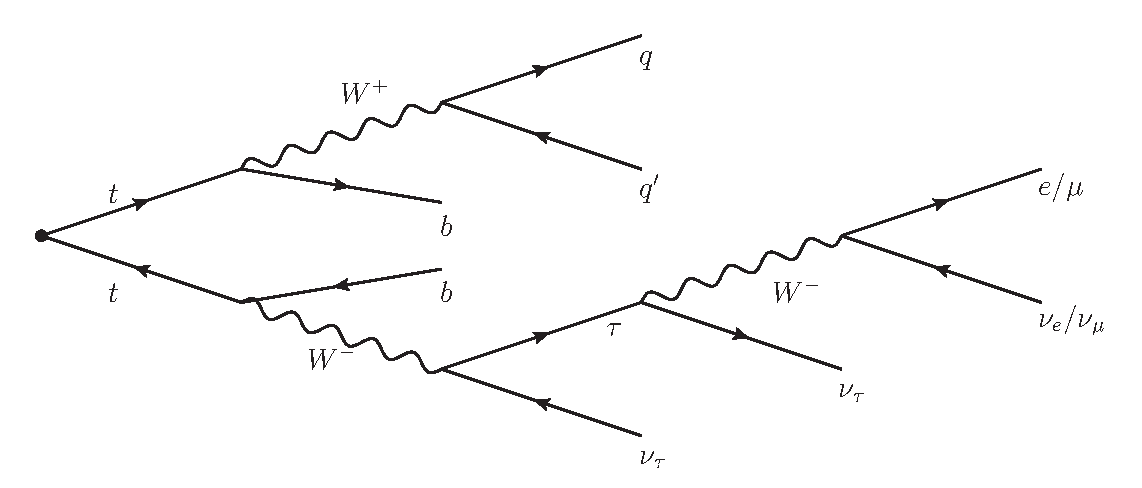
\includegraphics[width=0.45\textwidth]{Chapters/07_08_09_Analysis/Images/feynman_diagrams/semileptonic_tau_to_lepton}
%	\caption{}
		\label{subfig:semileptonic_tau_events}
		}
	\subfloat[]{
		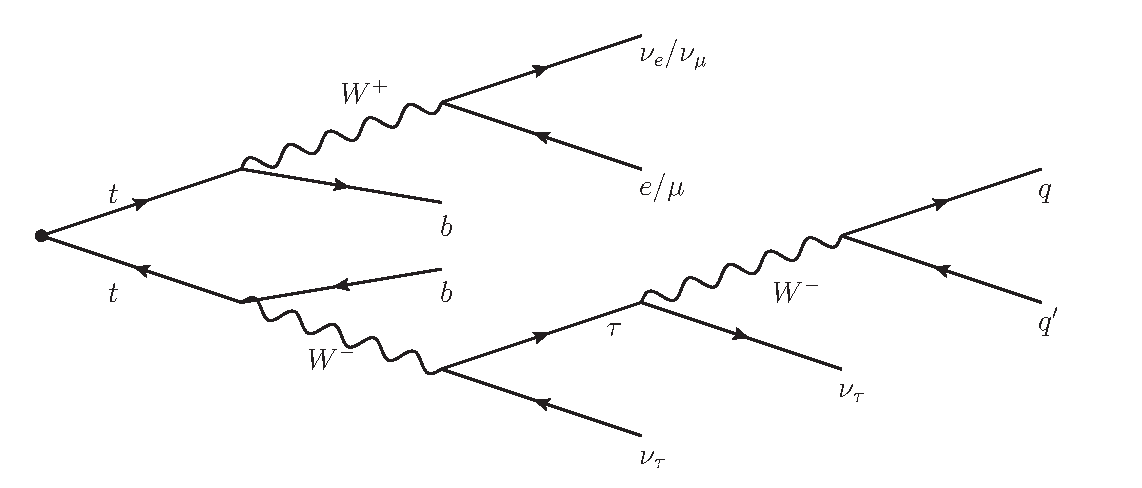
\includegraphics[width=0.45\textwidth]{Chapters/07_08_09_Analysis/Images/feynman_diagrams/dileptonic_tau_to_quarks}		
		\label{subfig:dileptonic_tau_events_to_quarks}
		}\\
	\subfloat[]{
		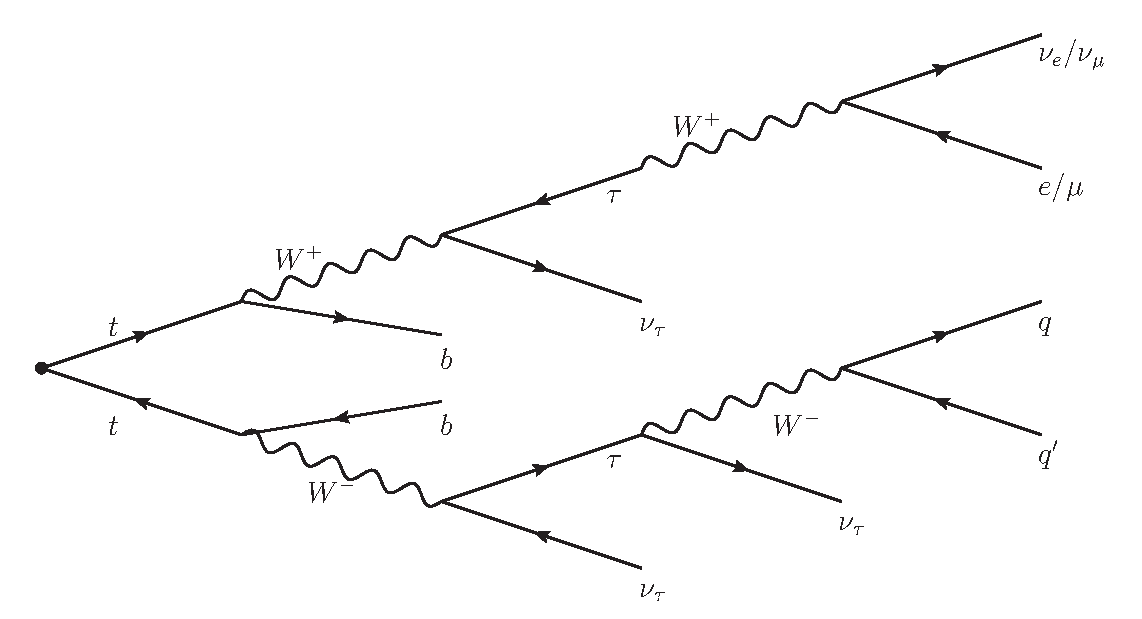
\includegraphics[width=0.45\textwidth]{Chapters/07_08_09_Analysis/Images/feynman_diagrams/dileptonic_tau_tau_to_quarks_and_leptons}
		\label{subfig:semileptonic_tau_events_to_quarks_and_leptons}
		}
	\caption[Diagrams of semi-leptonic and dileptonic $\tau$ events.]{Feynman diagrams of semi-leptonic $\tau$
	events (a), dileptonic events with one $\tau$ lepton (b) and dileptonic events with two $\tau$ leptons (c).}
	\label{fig:tau_diagrams}
\end{figure}

The first of these, where the leptonically decaying \W boson from a semi-leptonic \ttbar decay decays to a tau
lepton and a tau neutrino, and the tau lepton then decays to another tau neutrino, an electron/muon and an
electron neutrino/muon neutrino via a virtual \W boson, can be disregarded for the tau energy systematic since
the leptonically decaying tau is indistinguishable from the signal electron+jets or muon+jets channels.
It is therefore not possible to include such an event in the calculation of the \met uncertainty by varying
the $\tau$ energy. The other two tau decay channels which potentially fake the signal and pass the \ttbar
signal selection are distinguishable and are included.

Fake events are removed by subtracting the fake distribution obtained from simulation. However, for the
systematic measurements with the tau energy varied up and down, the same fake distribution shape is subtracted
as in the nominal measurement. The left-hand plot in Figure~\ref{fig:tau_shape_number_comparison} compares the
numbers of events in the signal and fake distributions from \ttbar simulation after selection.
Based on this, an evaluation of the ratio of fake events to the number of reconstructed \ttbar events in
simulation has been calculated to be approximately 14\% (13.5\% in electron channel and 13.9\% in muon
channel). The large component of taus in the fake distribution leads to the larger systematic uncertainties
(up to $\approx6-7\%$) as a result of varying the tau energy, while the effect of varying the electron and
muon energies is not so pronounced because there are not many electrons or muons in the fake collection (a
dileptonic \ttbar event with $ee$, $e\mu$ or $\mu\mu$ would have to be misreconstructed as a semi-leptonic
event for this to happen). A comparison of the shapes of the fake and the signal \met distributions from
simulation is also shown on the right in Figure~\ref{fig:tau_shape_number_comparison}. It can be seen that the
relative contribution from fakes increases towards higher values of \met, which leads to the observed increase
in the systematic uncertainty due to the uncertainty in the tau energy towards higher bins of \met.

\begin{figure}[hbtp]
    \centering
     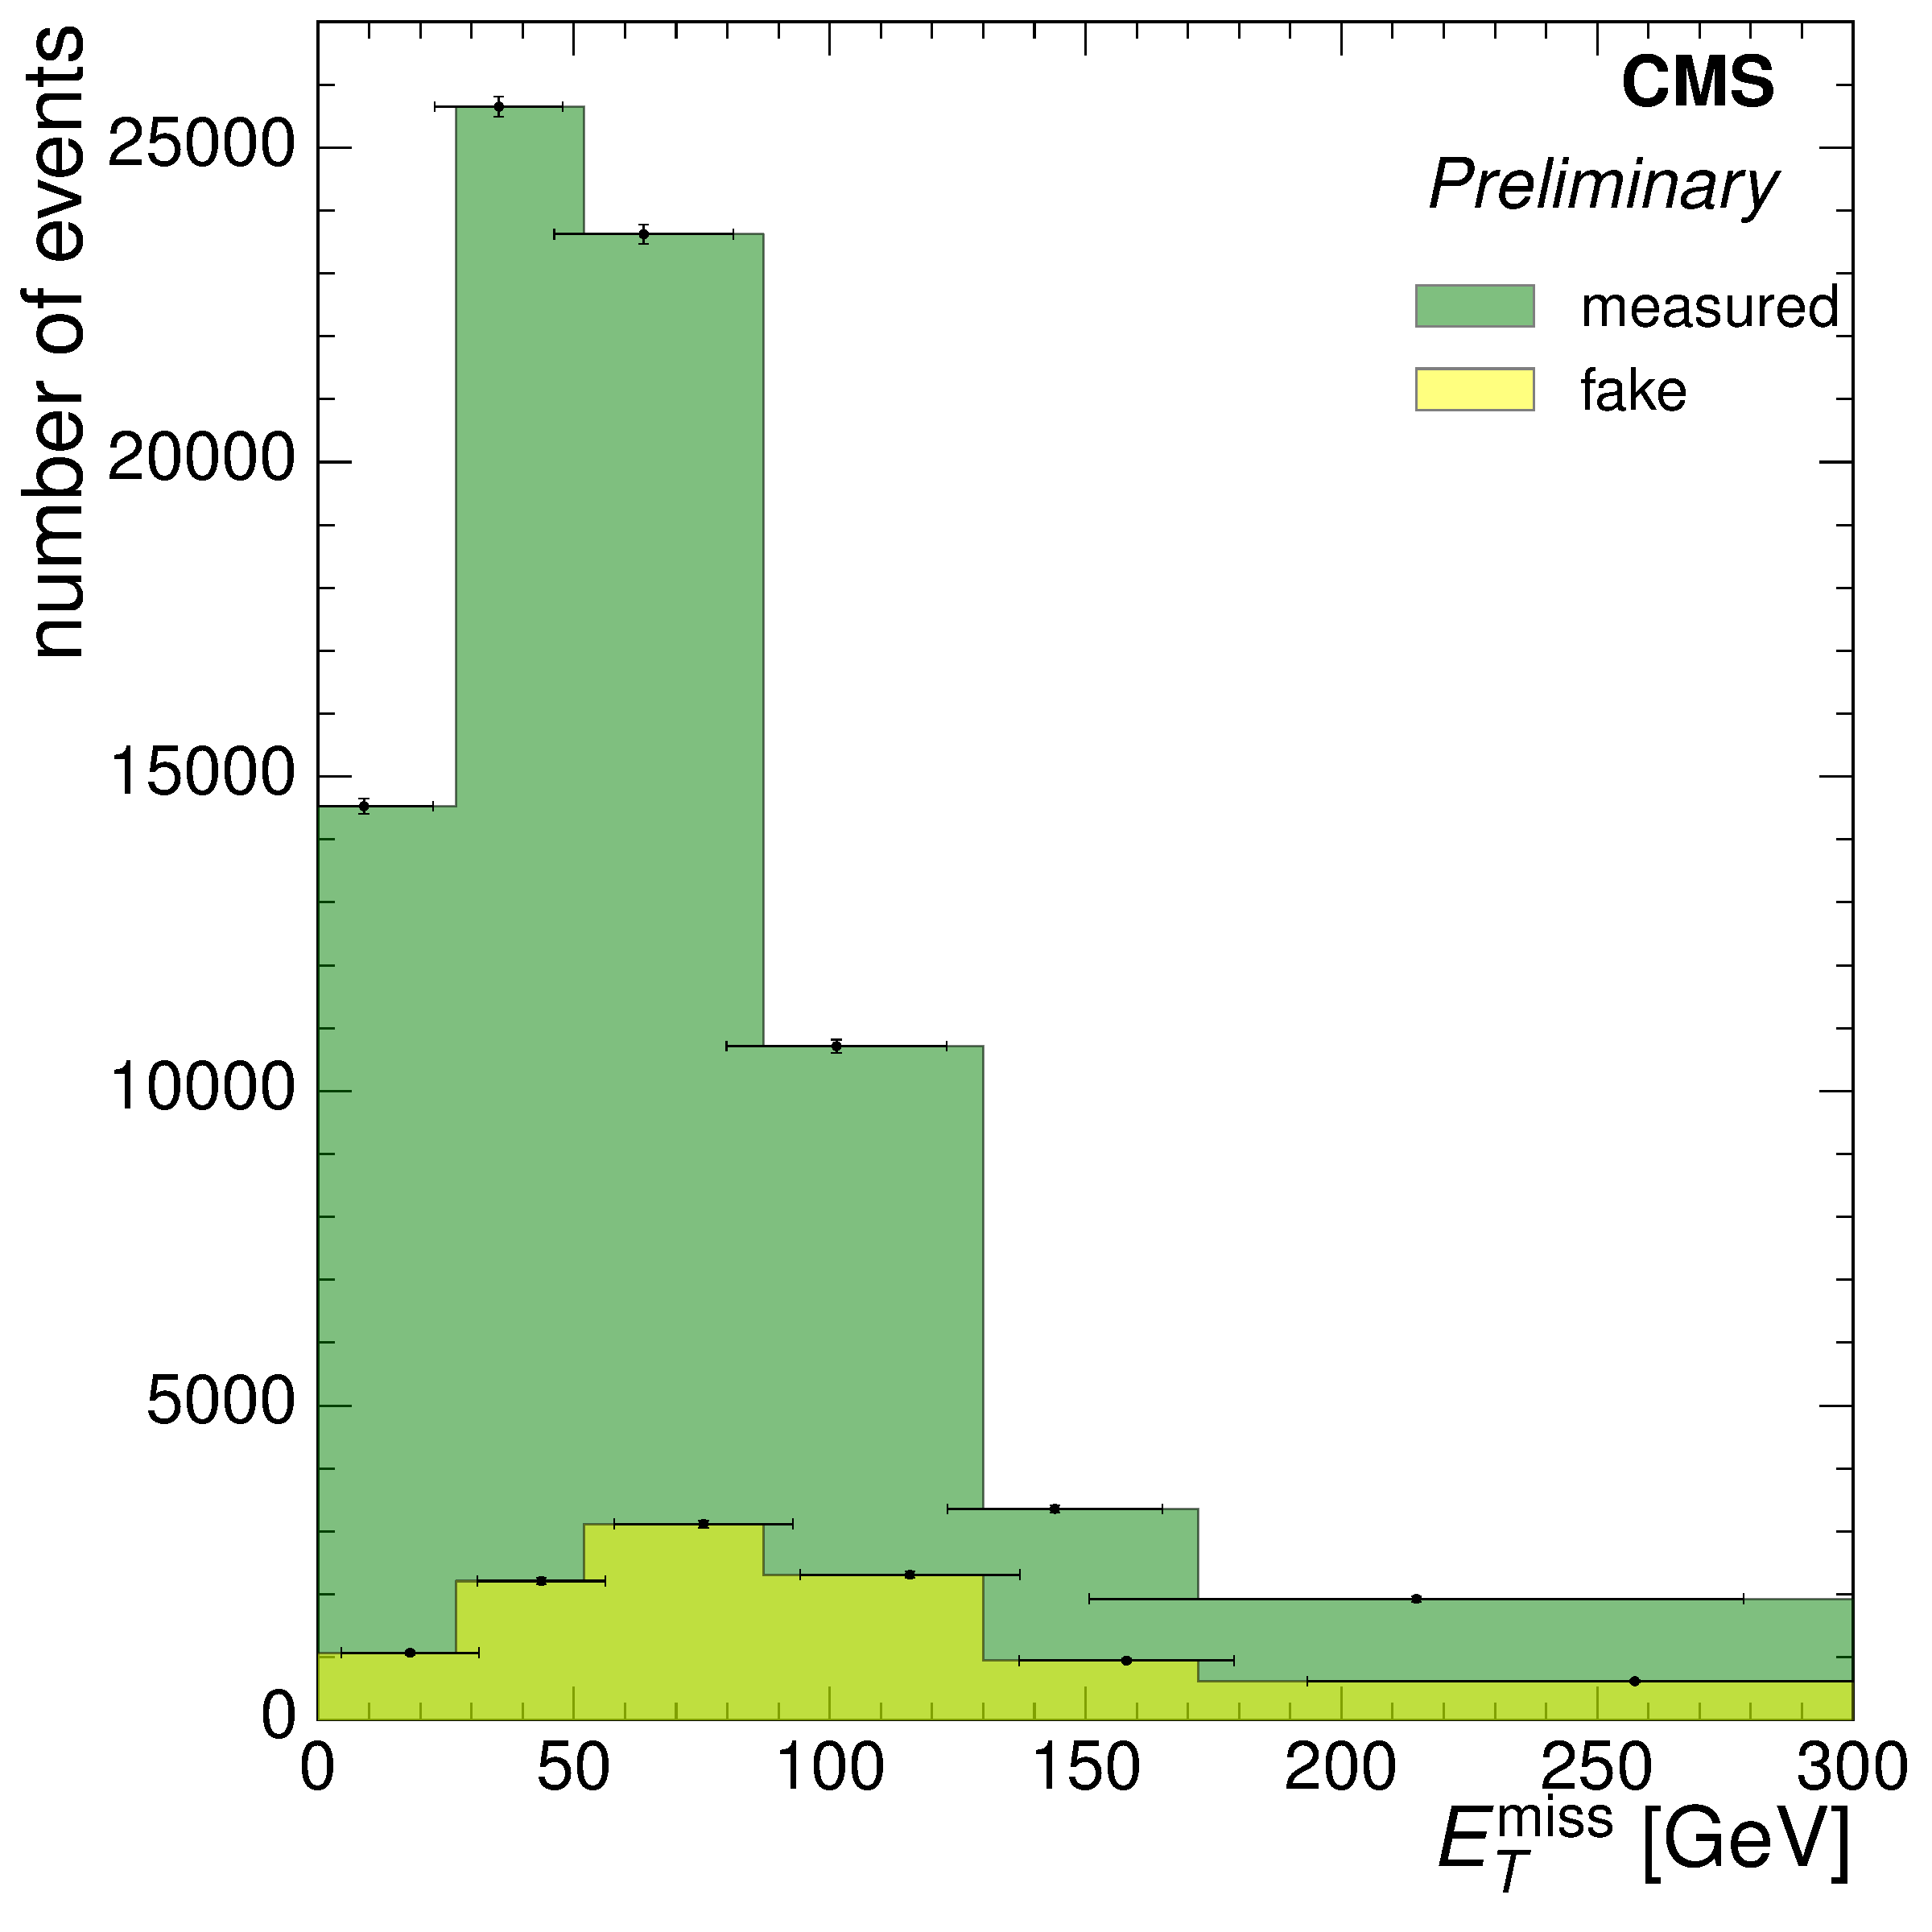
\includegraphics[width=0.48\textwidth]{Chapters/07_08_09_Analysis/Images/tau_cross_checks/comparison_measured_fake_TTJets_normalised_to_nevents.pdf}
     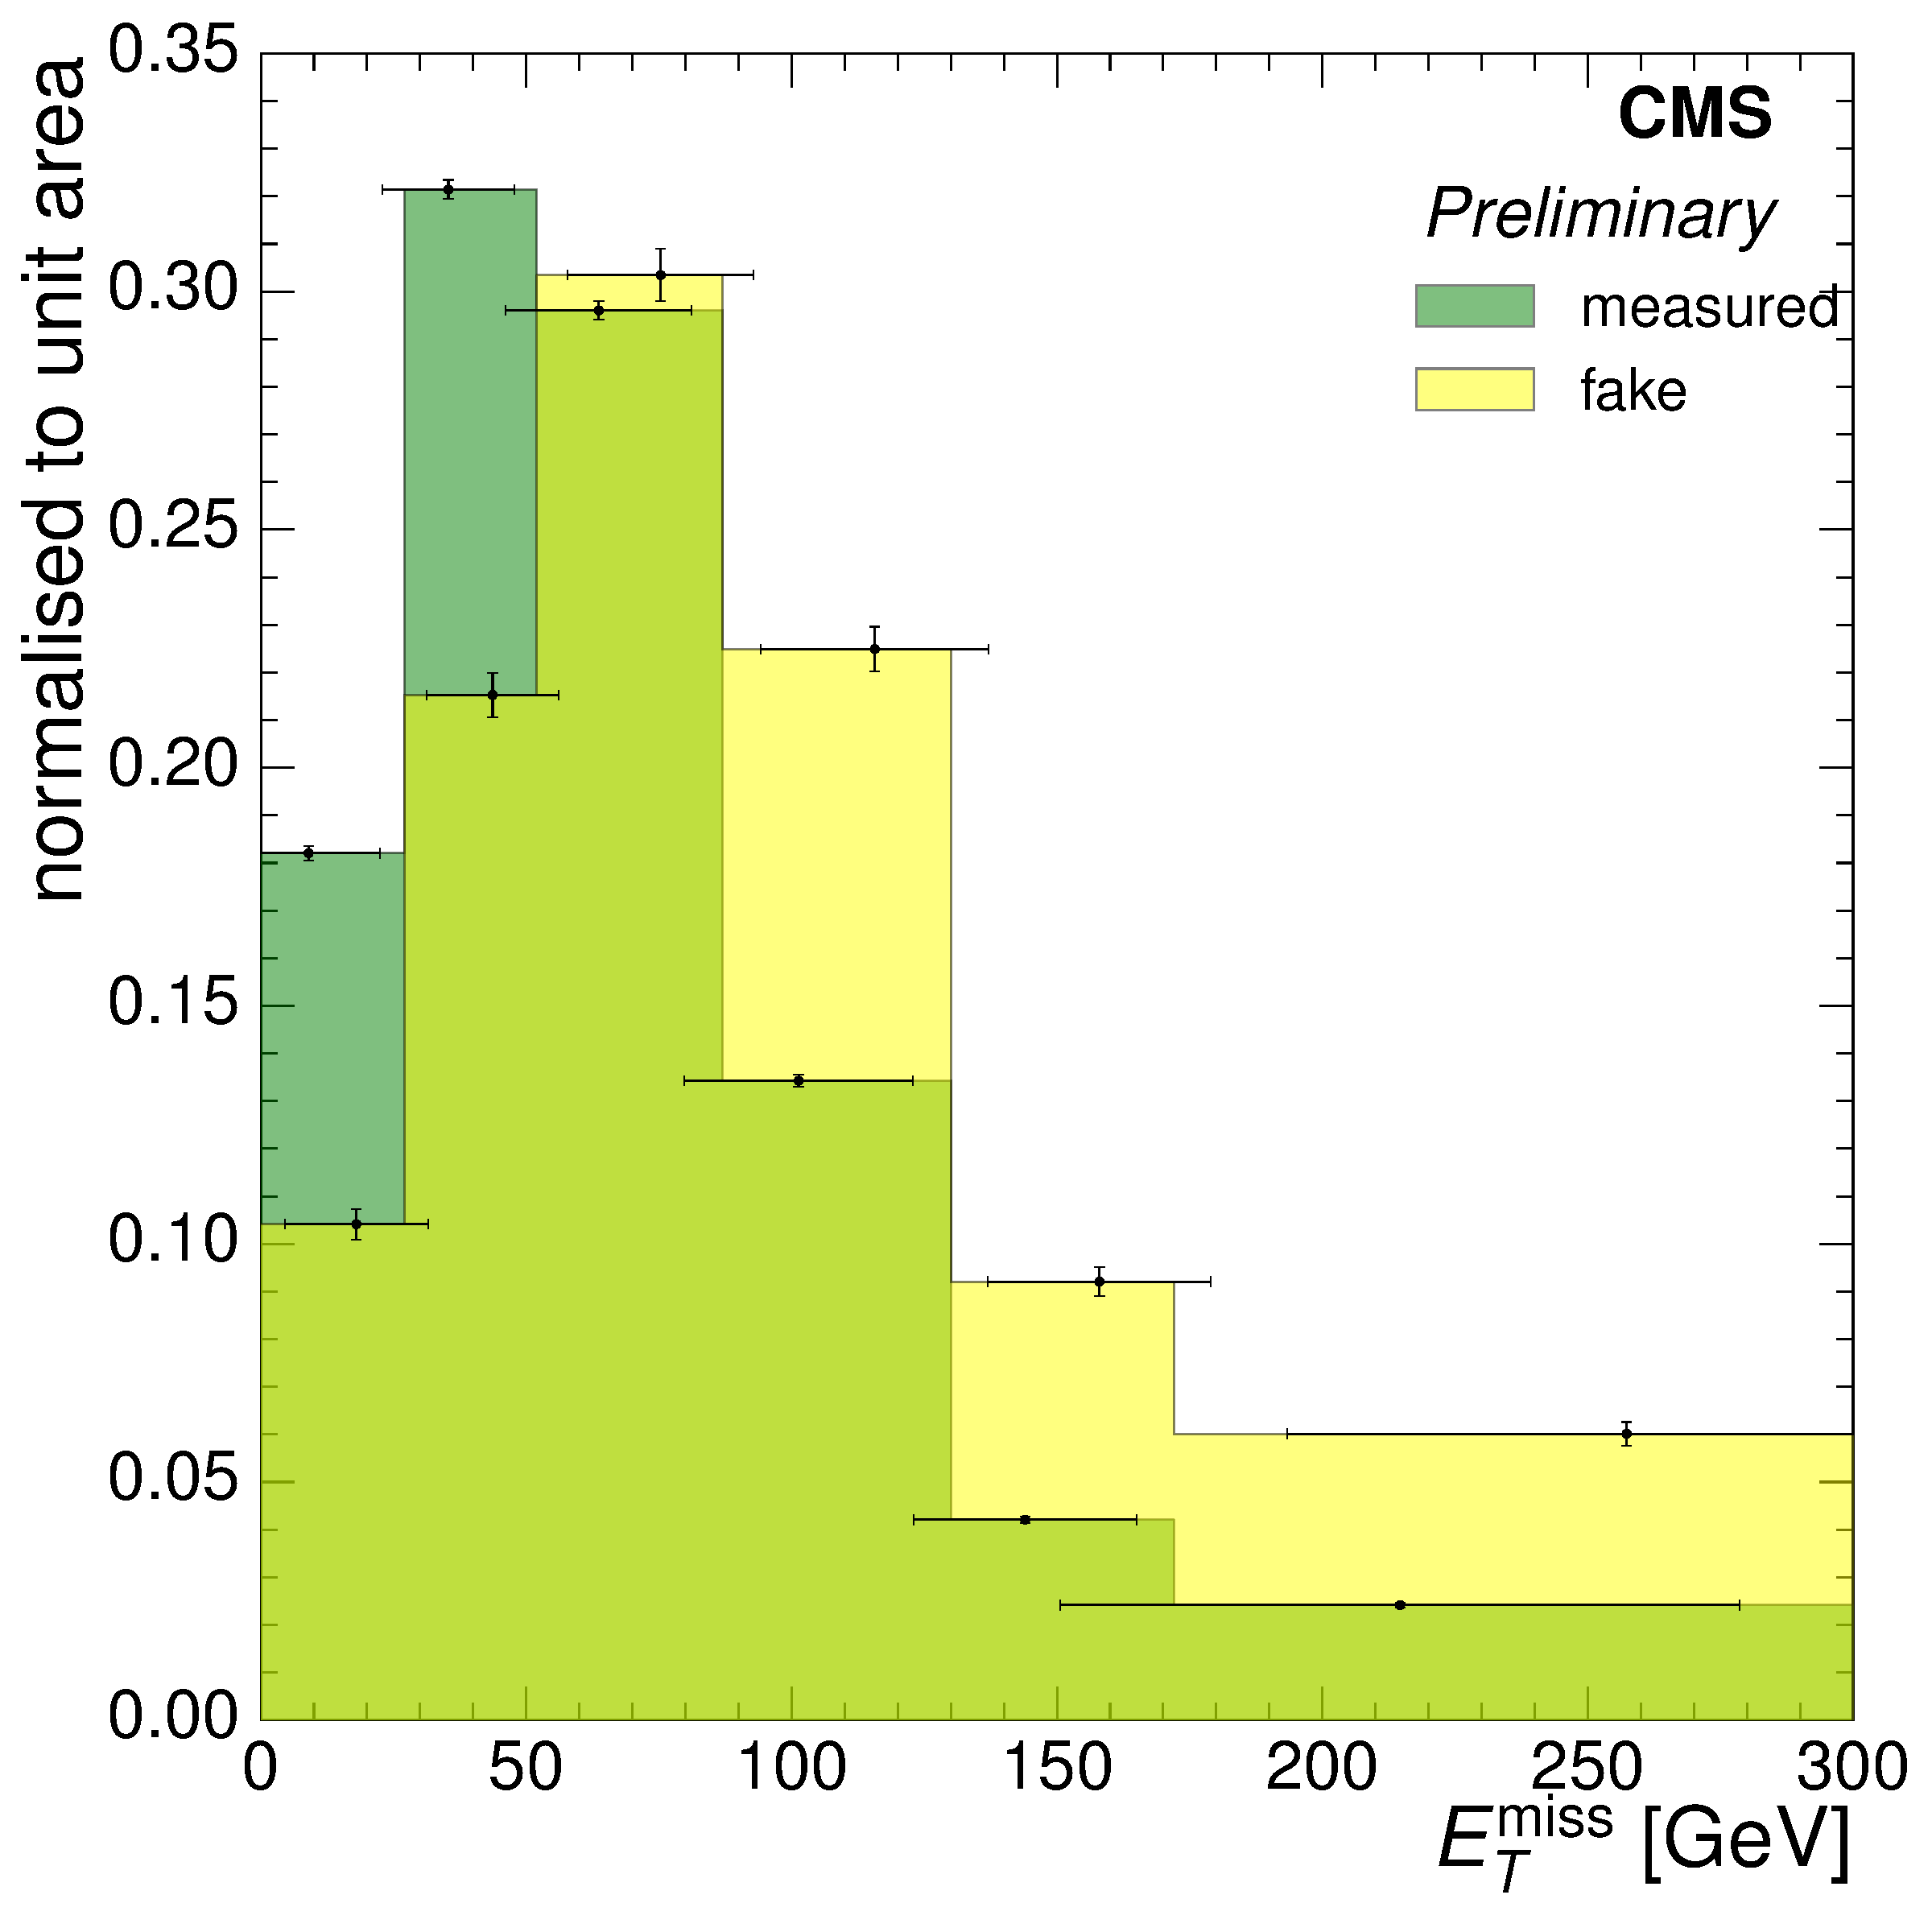
\includegraphics[width=0.48\textwidth]{Chapters/07_08_09_Analysis/Images/tau_cross_checks/comparison_measured_fake_TTJets_normalised_to_one_without_ratio.pdf}\hfill
     \caption[Comparison of the signal and fake distributions in the \met variable from semi-leptonic \ttbar
	 events in the electron+jets channel at $\roots=8\TeV$.]{Comparison of the signal and fake distributions from
	 semi-leptonic \ttbar events after selection in simulation in the electron+jets channel at $\roots=8\TeV$
	 normalised to the numbers of events (left) and normalised to one (right).}
     \label{fig:tau_shape_number_comparison}
\end{figure}

Furthermore, the difference between the tau energy down ($-1\sigma$) variation and the nominal measurements in
the \met variable before fitting and unfolding is shown in Figure~\ref{fig:tau_down_comparison}. In the
highest \met bin, the difference is approximately 6\%, and this value remains approximately constant after
fitting and unfolding. The significant effect of varying the tau energy is therefore unlikely to be an
artifact of the fitting and/or unfolding procedure, but a real difference in the number of events.

\begin{figure}[hbtp]
    \centering
     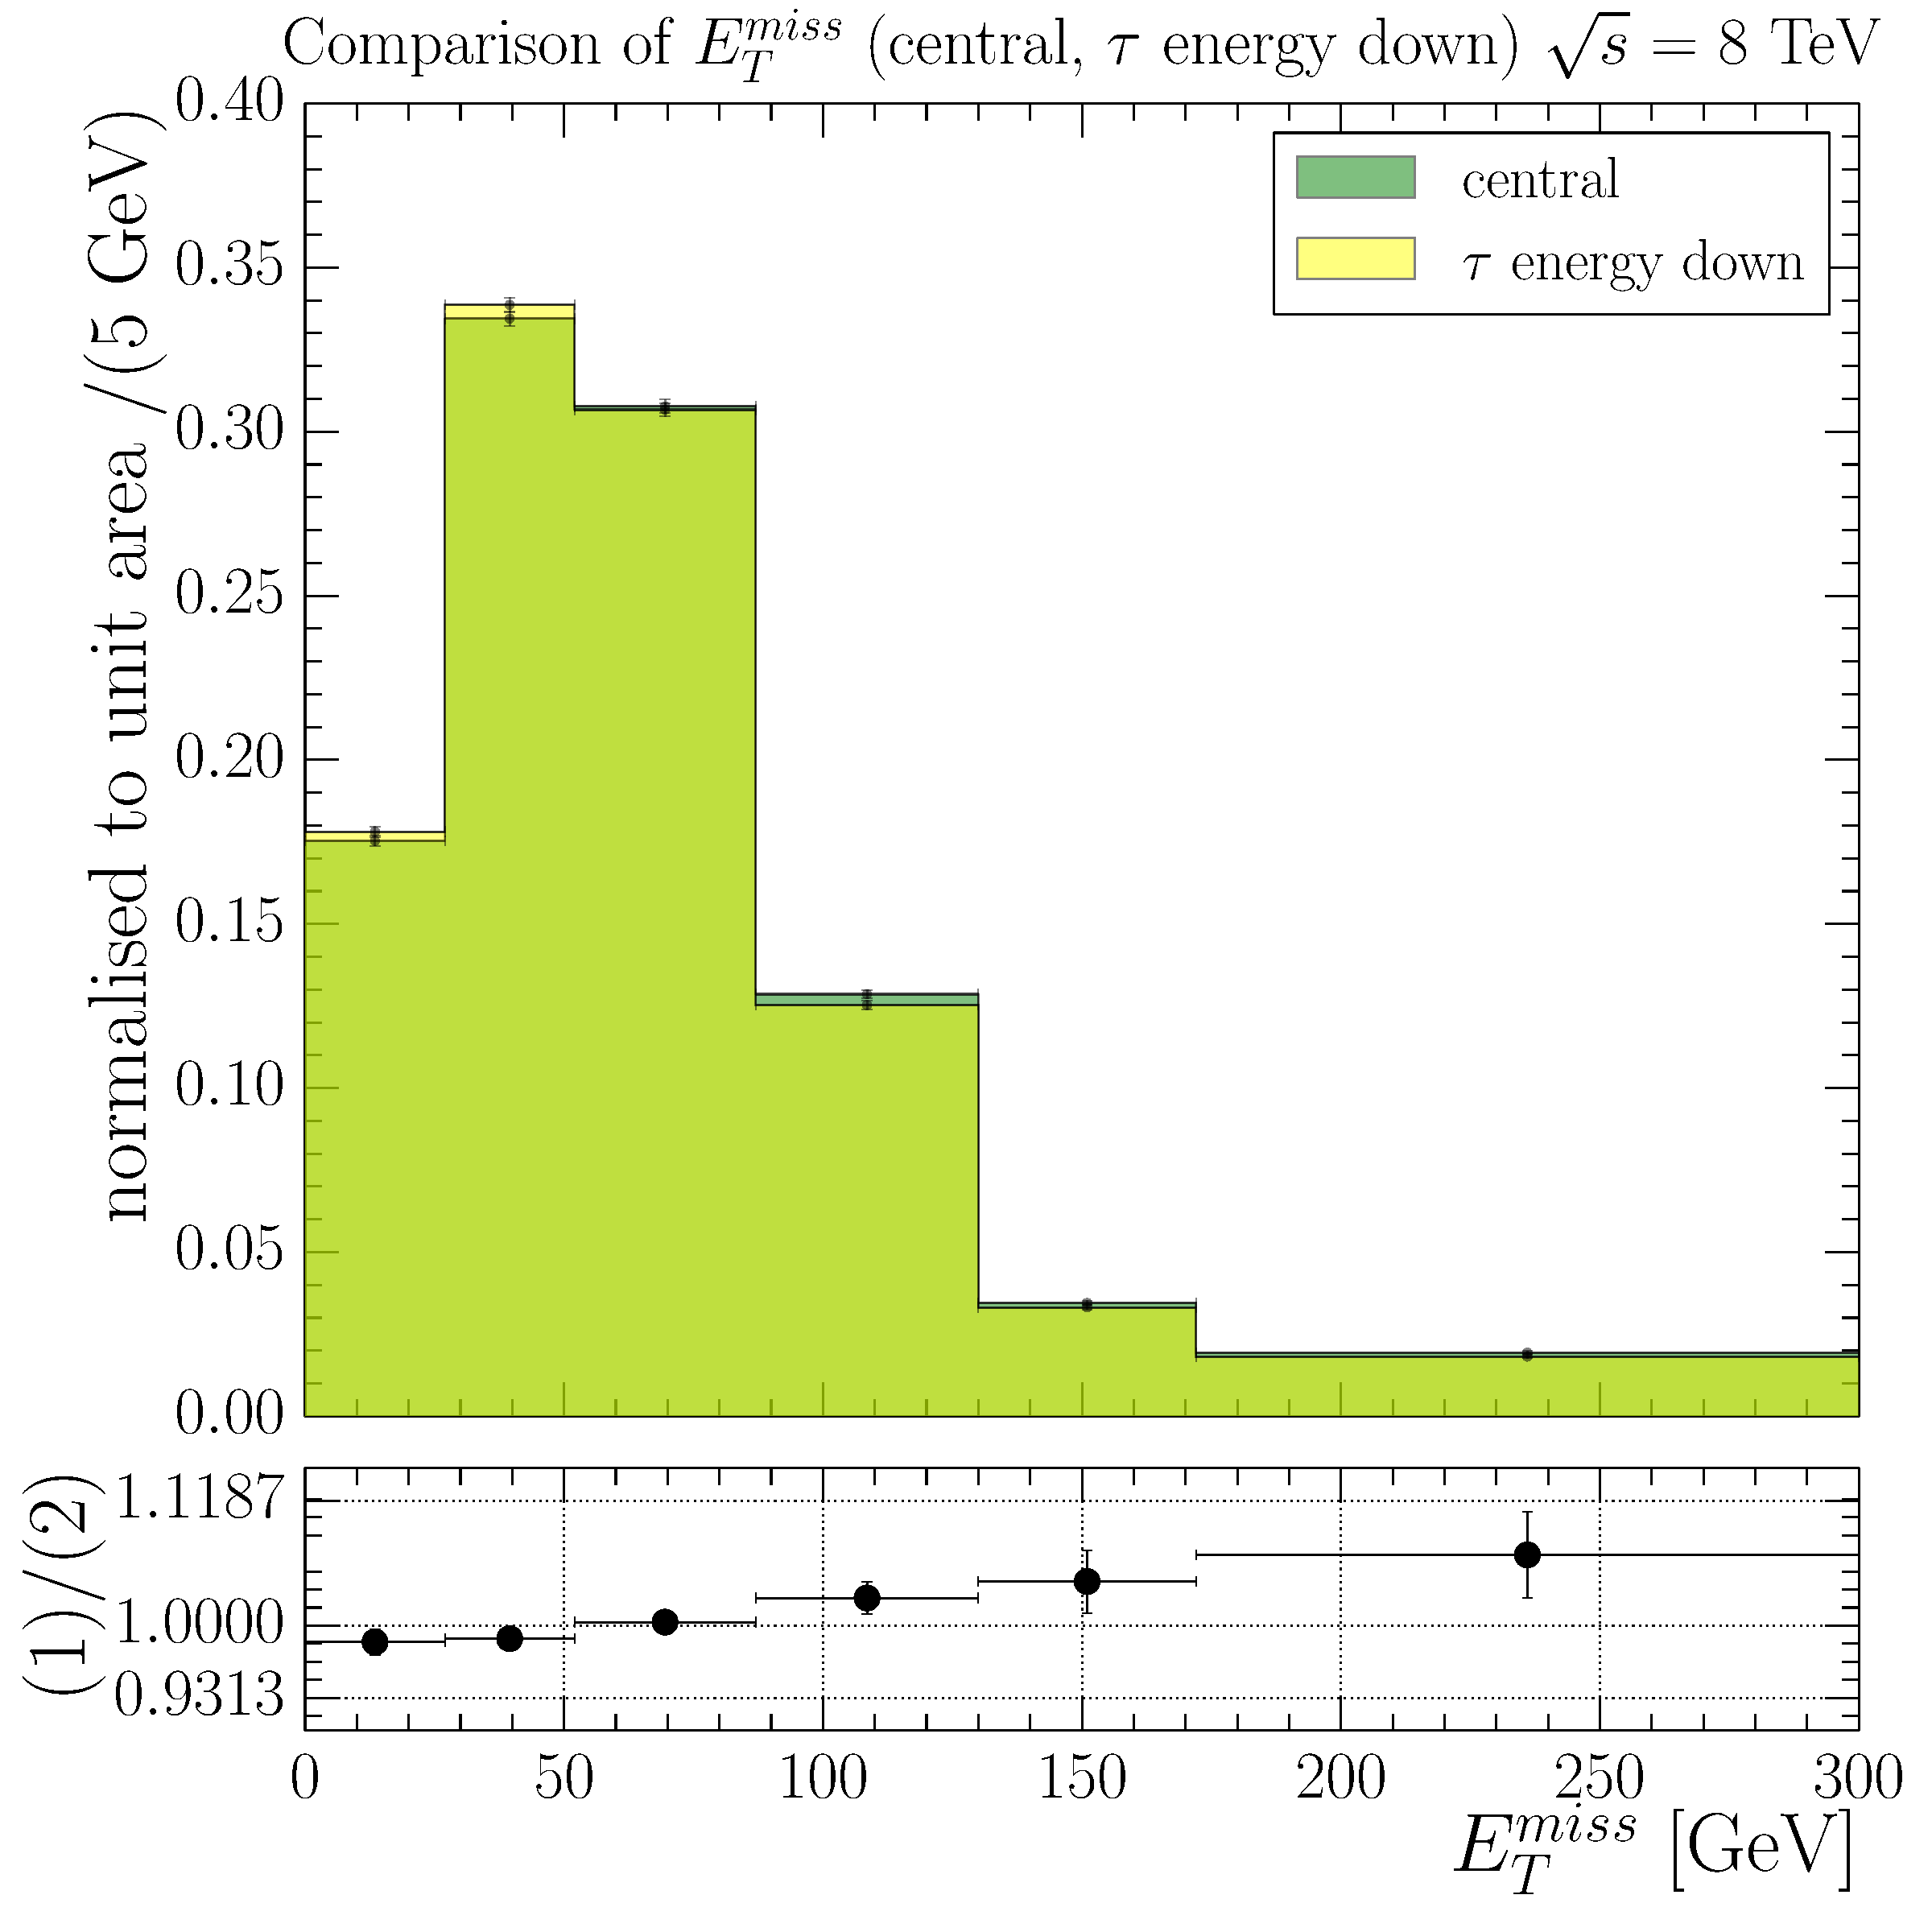
\includegraphics[width=0.48\textwidth]{Chapters/07_08_09_Analysis/Images/tau_cross_checks/compare_central_MET_to_tau_energy_down_asym_bins_electron_channel_data.pdf}\hfill
     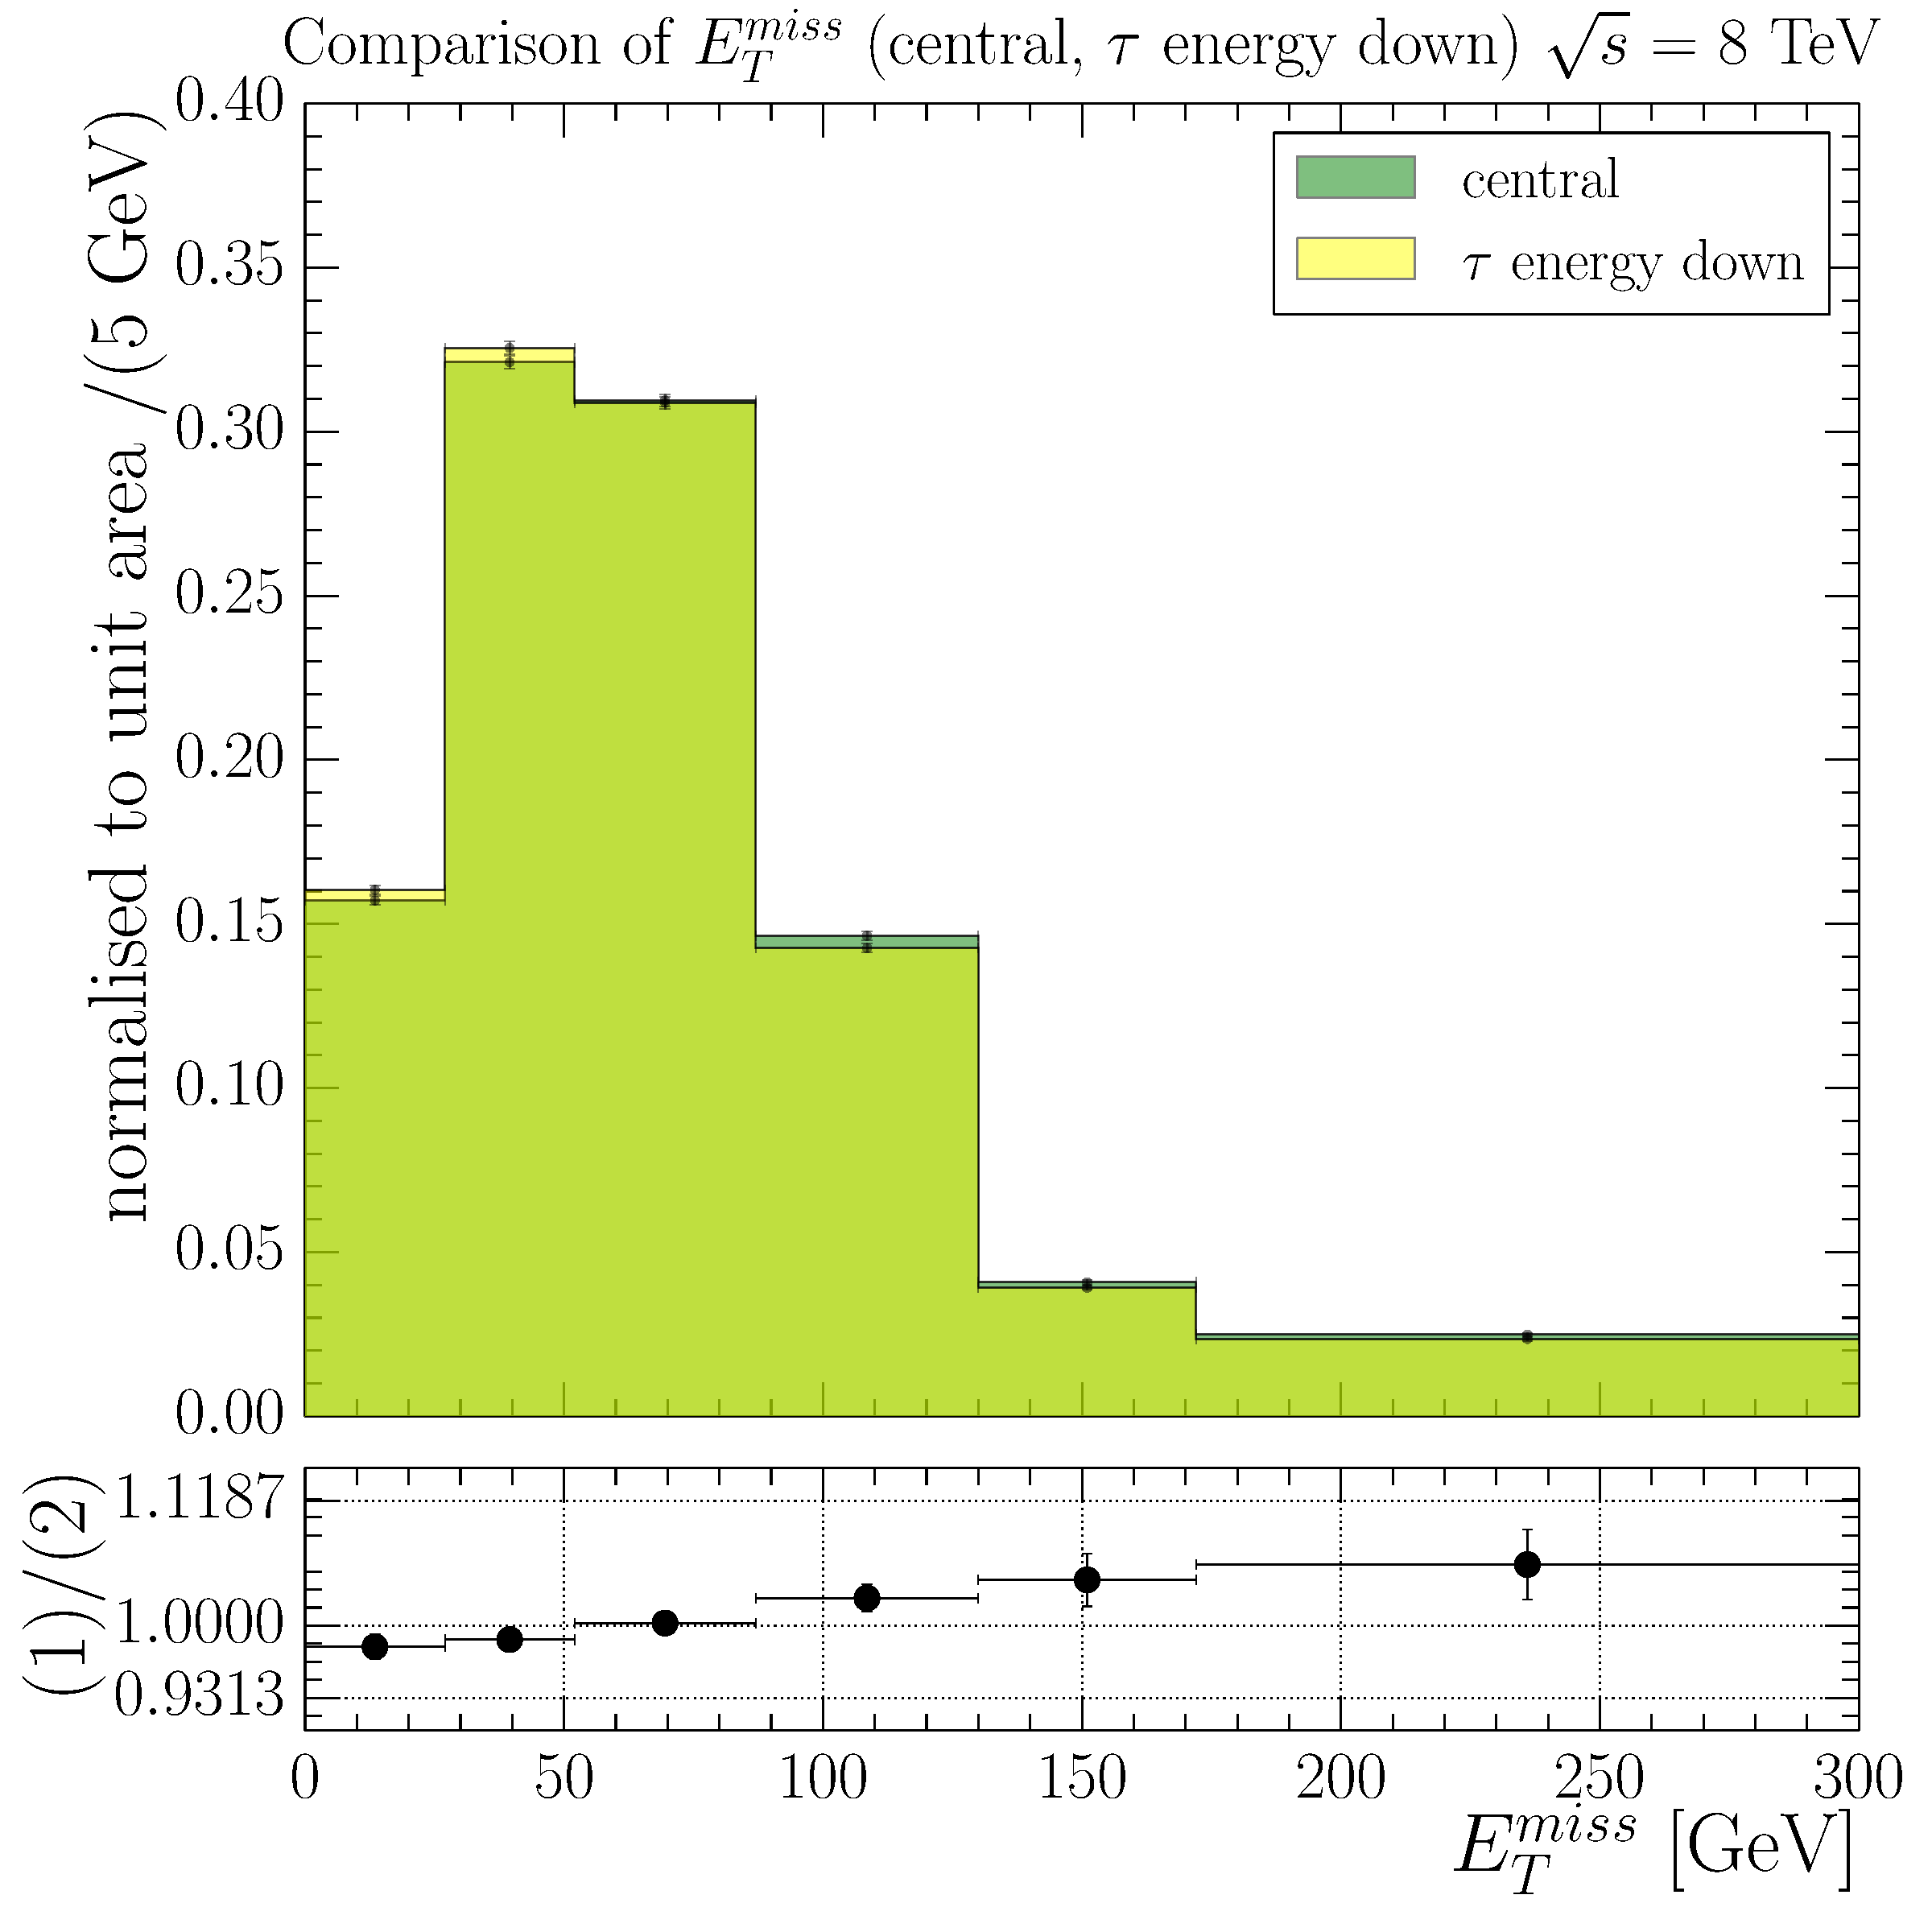
\includegraphics[width=0.48\textwidth]{Chapters/07_08_09_Analysis/Images/tau_cross_checks/compare_central_MET_to_tau_energy_down_asym_bins_electron_channel_TTJet.pdf}
     \caption[Comparison of the \met distributions in the nominal measurement and in the tau energy down
     variation in data and in simulation.]{Comparison of the \met distributions in the nominal measurement and
     in the tau energy down variation before fitting and unfolding in data (left) and in \ttbar simulation
     (right) at $\roots=8\TeV$}
     \label{fig:tau_down_comparison}
\end{figure}
 
Other small sources of experimental uncertainty include the non-clustered energy uncertainty (which refers to
fluctuations in deposits in the electromagnetic calorimeter that are not included in jet clusters), the
matching threshold and factorisation and normalisation scale uncertainties in \WpJets and \ZpJets events,
pileup uncertainty, the QCD template shape uncertainty, and the efficiency of electron, muon and \btagging in
the selection process.

Rate changing systematics such as the uncertainty on the luminosity and on the theoretical cross sections of
the signal and background processes have a negligible effect on the final result, since they cancel in the
final normalised measurements.

\FloatBarrier

\subsection{Theoretical Uncertainties}
\label{ss:theoretical_uncertainties}

\subsubsection{7\TeV V+Jets theory systematic template}
\label{sss:7TeV_vjets_theory_systematic_template}

The factorisation and normalisation scale ($Q^{2}$ up/down) uncertainty is evaluated using simulation samples
produced with the scale varied by factors of 2 (up) and 0.5 (down). This has been evaluated to be one of the
dominating uncertainties in this analysis. The uncertainty in the matching threshold (matching up/down) for
\ttbar events is evaluated in the same way.

Unfortunately, Monte Carlo simulation for theoretical systematic uncertainties at $\roots=7\TeV$ have not
been made available for W+jets and Z+jets processes. However, it can be seen in
Figure~\ref{fig:wjets_7TeV_8TeV_comparison} that the W+jets template shapes at $\roots=7\TeV$ and
$\roots=8\TeV$ are similar. The V+jets template shapes used to evaluate these theoretical systematics are
therefore obtained from $\roots=8\TeV$ theoretical systematic datasets, and then scaled to the normalisation
in the nominal sample at $\roots=7\TeV$.

\begin{figure}[hbtp]
    \centering
     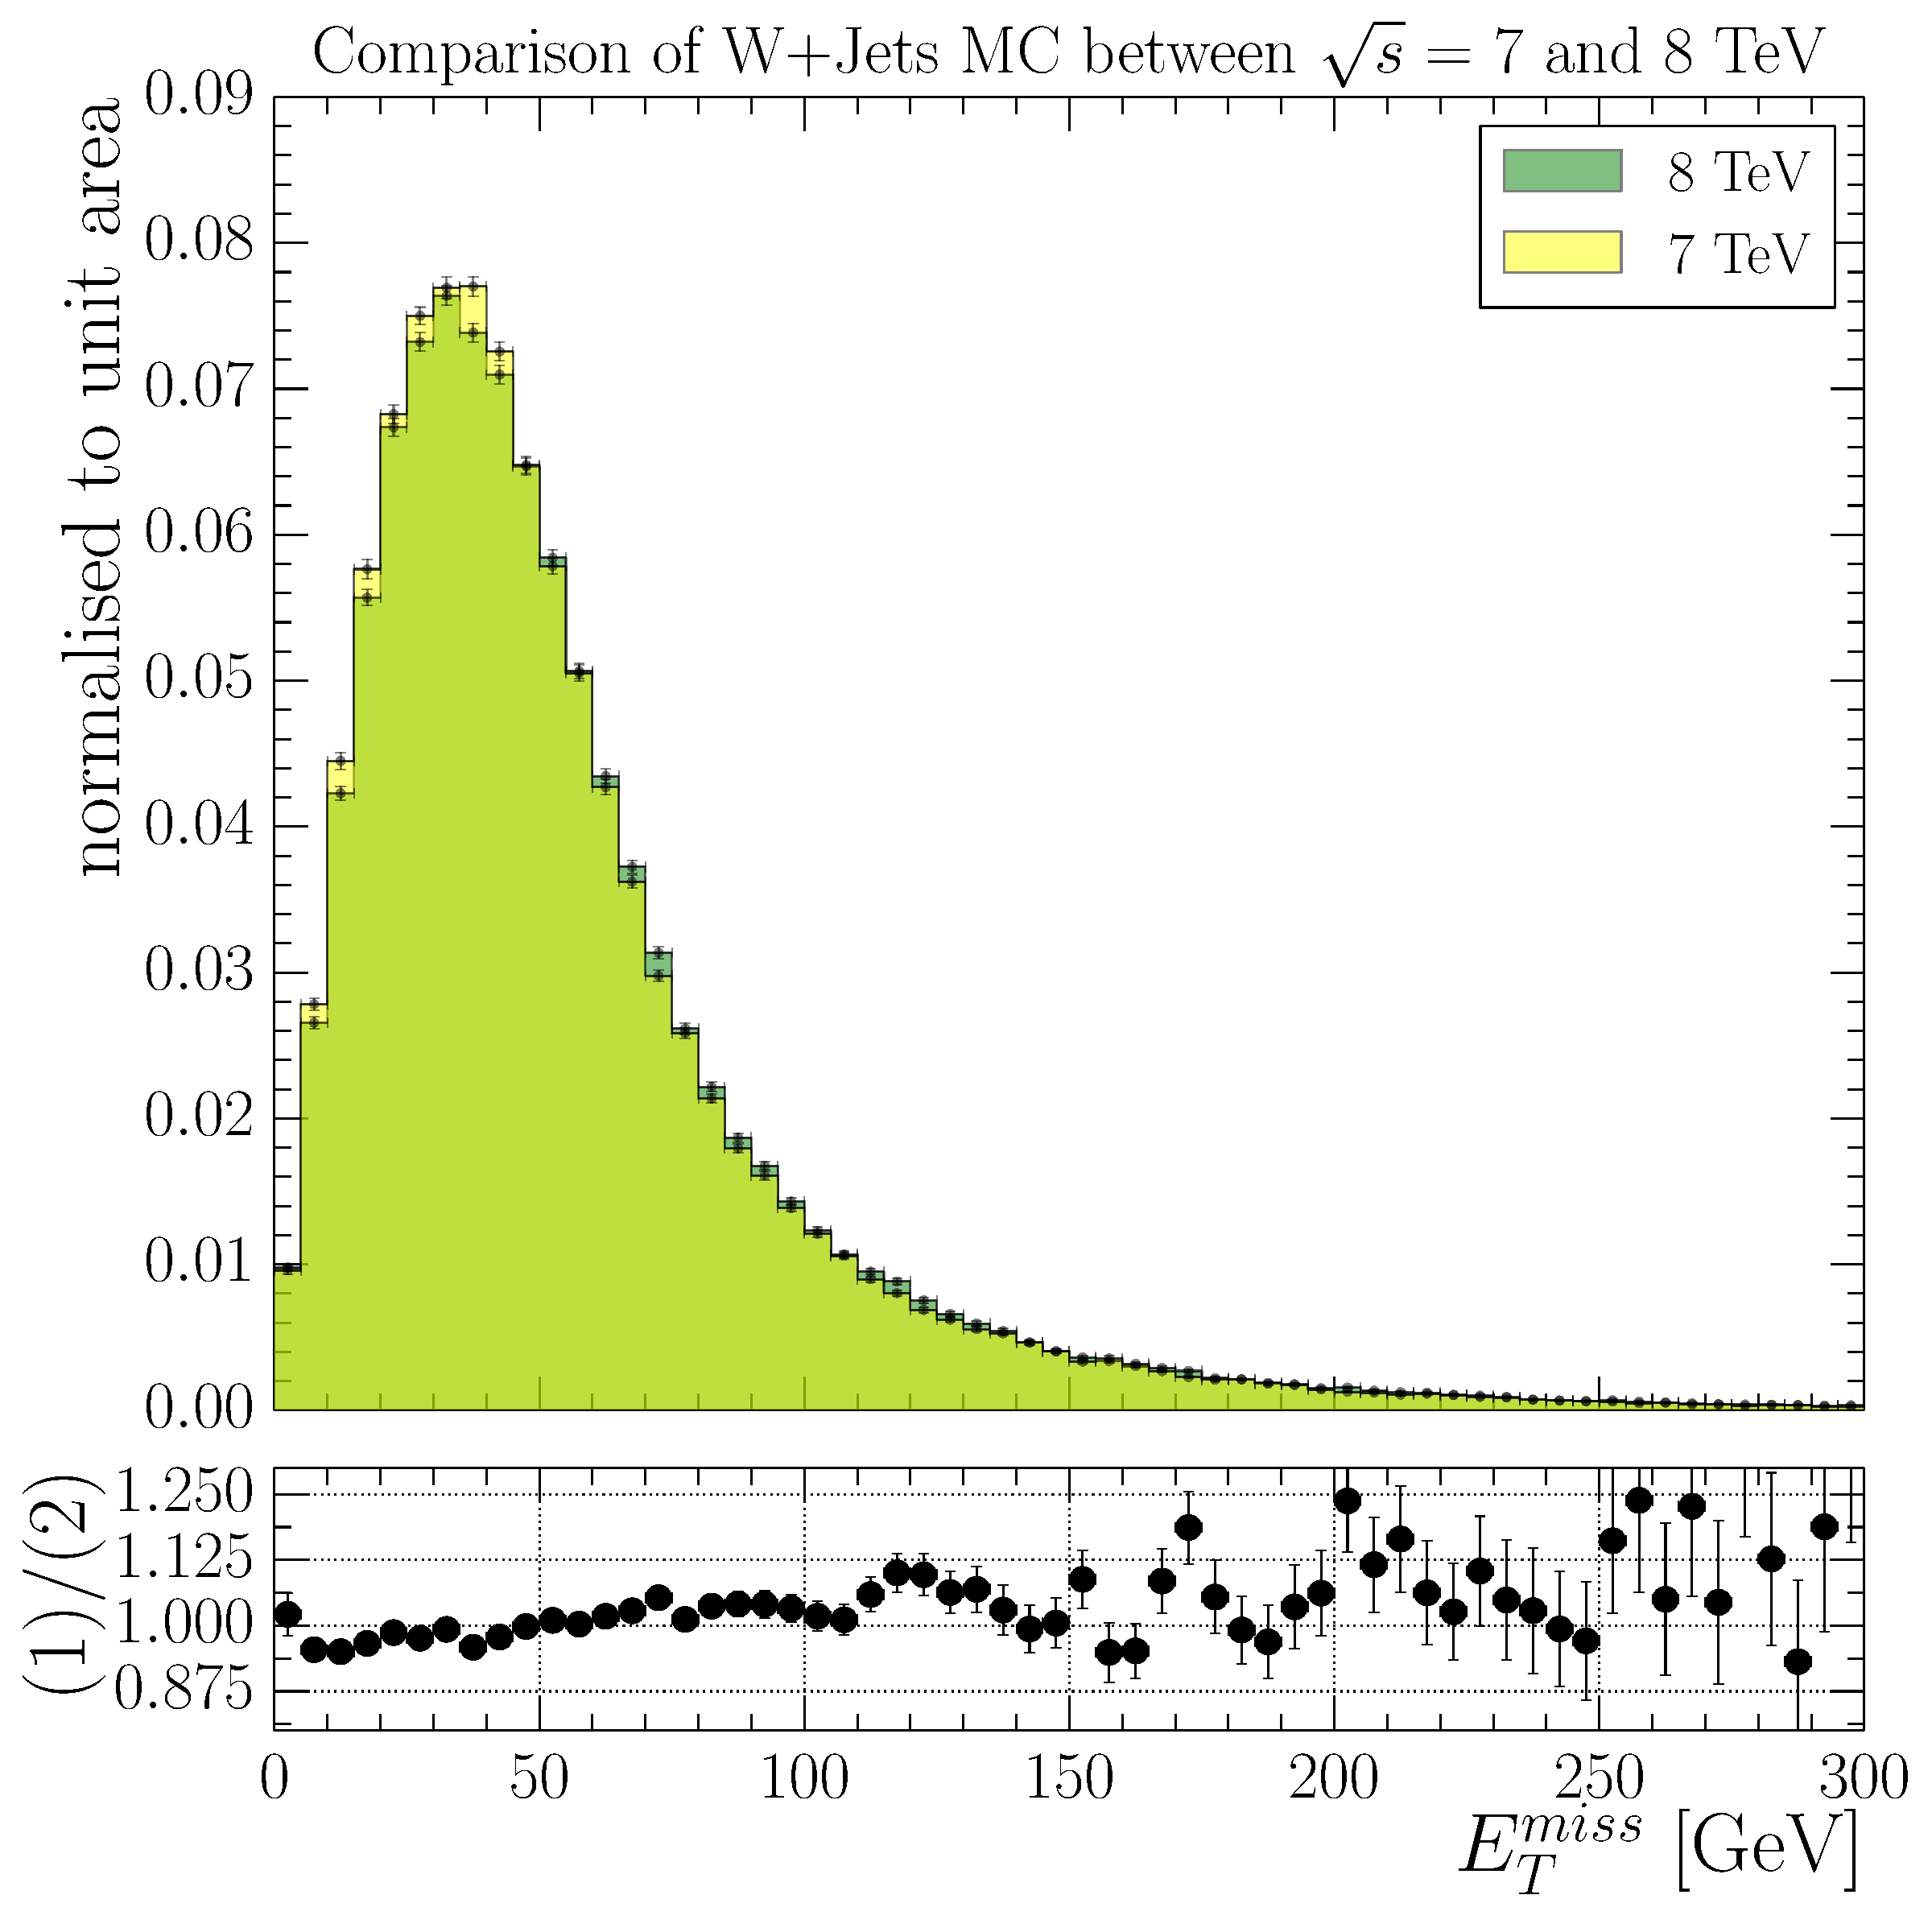
\includegraphics[width=0.48\textwidth]{Chapters/07_08_09_Analysis/Images/WJets_comparison/TTbar_plus_X_analysis_EPlusJets_Refselection_MET_patType1CorrectedPFMet_MET_0orMoreBtag.pdf}\hfill
     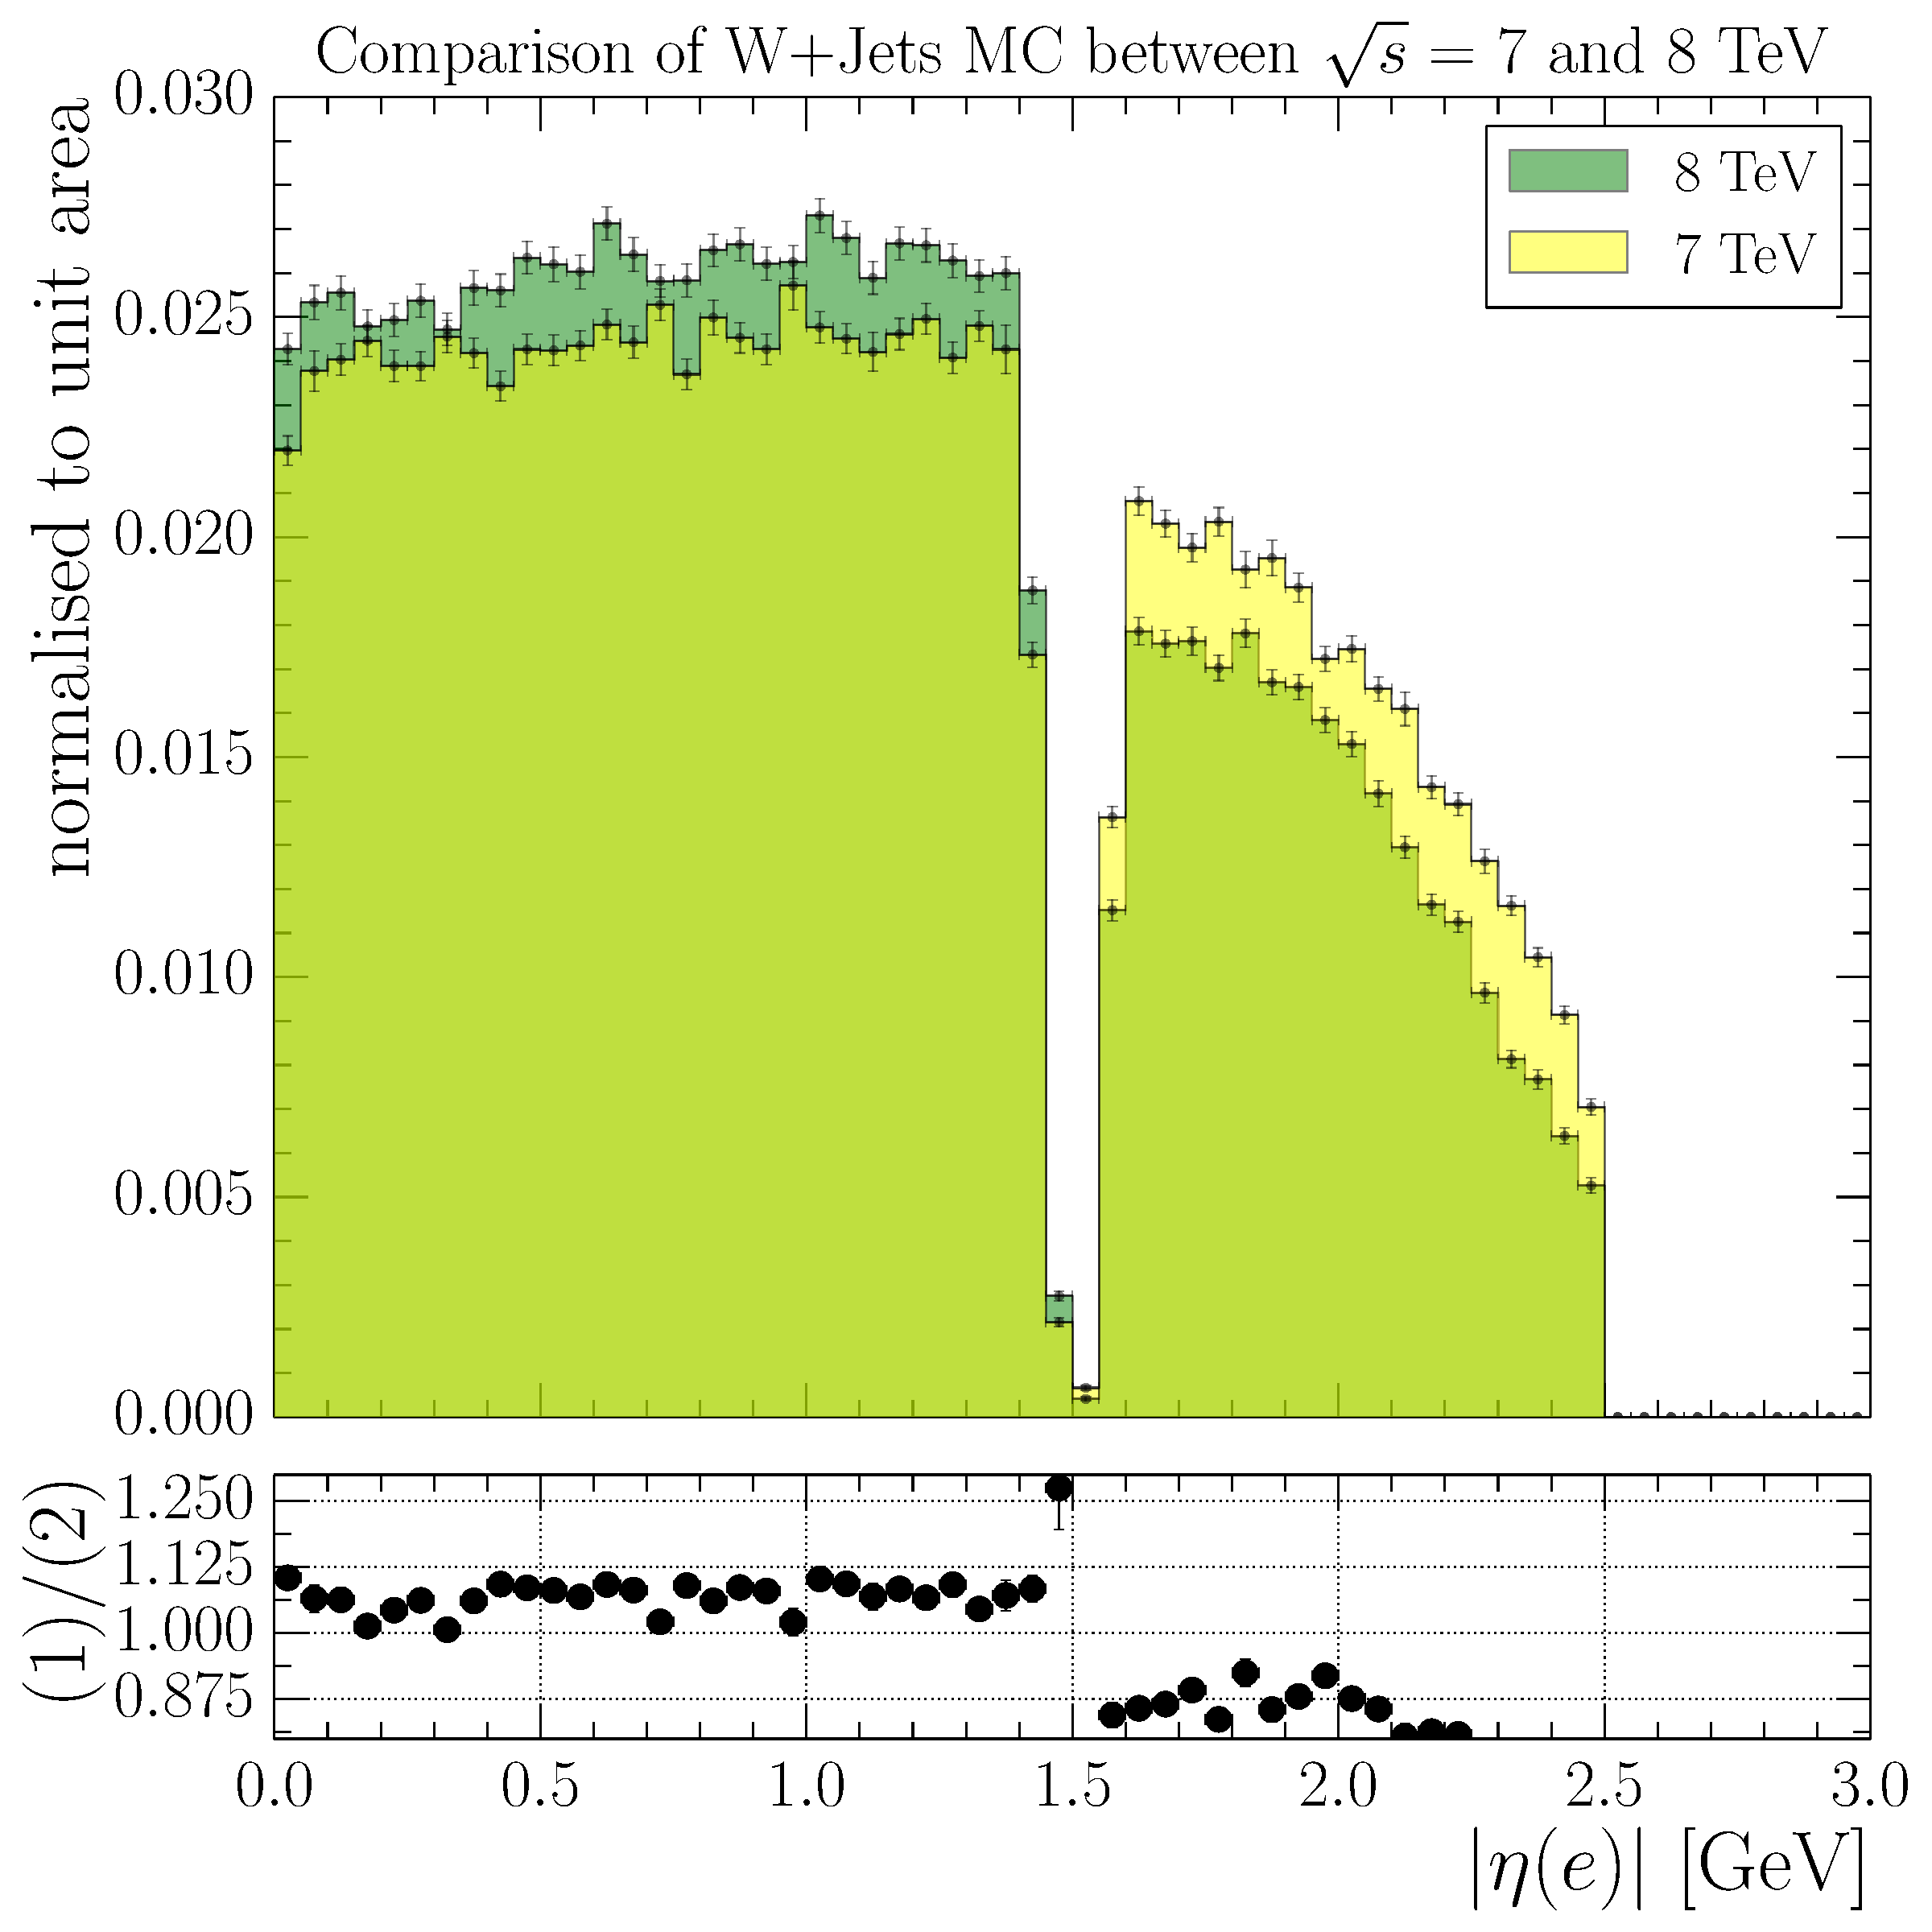
\includegraphics[width=0.48\textwidth]{Chapters/07_08_09_Analysis/Images/WJets_comparison/TTbar_plus_X_analysis_EPlusJets_Refselection_Electron_electron_AbsEta_0orMoreBtag.pdf}\\
	 \caption[\met and electron \abseta shape comparison of W+jets templates in $\roots=7\TeV$ and
	 $\roots=8\TeV$ in the electron+jets channel.]{Shape comparison of W+jets templates in $\roots=7\TeV$ and
	 $\roots=8\TeV$ Monte Carlo simulation for \met (left) and electron \abseta (right) in the electron+jets
	 channel.}
     \label{fig:wjets_7TeV_8TeV_comparison}
\end{figure}

\subsubsection{Hadronisation Uncertainty}
\label{sss:hadronisation_uncertainty}
The uncertainty due to hadronisation modelling is evaluated by comparing the results using \ttbar simulation
from the \POWHEG1 generator with \PYTHIA modelling the hadron showering (\POWHEGPYTHIA1), with a sample
generated using the same \POWHEG1 generator with \HERWIG carrying out the hadronisation modelling
(\POWHEGHERWIG1). The difference between the \PYTHIA and \HERWIG samples is scaled to the nominal measurement
and taken as the hadronisation uncertainty. At $\roots=7\TeV$, since these samples are not available, the
hadronisation uncertainty is obtained by scaling the relative uncertainty at $\roots=8\TeV$ to the central
$\roots=7\TeV$ result. All variables, and in particular those sensitive to hadronic aspects of an event such
as \HT and \st, are significantly affected by this systematic, with a larger uncertainty in lower bins of the
primary variables. %TODO:check this is still the case

\subsubsection{PDF Uncertainties}
\label{sss:PDF_uncertainties}
The uncertainty on the measurements as a result of the uncertainty on the choice of proton PDFs is evaluated
by reweighting the central \MADGRAPH sample with 44 distinct weights (22 orthogonal variables, each of which
can be varied up and down according to their uncertainties) from the CTEQ 6.6 PDF sets~\cite{Nadolsky:2008zw},
according to the PDF4LHC recommendation~\cite{Botje:2011sn,Alekhin:2011sk}. The analysis is repeated with each
variation, and the maximum of all the up and down variations summed in quadrature is taken as the PDF
systematic uncertainty.

\subsubsection{Top Quark Mass Uncertainty}
\label{sss:top_quark_mass_uncertainty}
The top quark mass uncertainty is evaluated using \ttbar samples produced with two different top quark masses
of 169.5\GeV and 173.5\GeV, and scaling the the error obtained using these samples to the top mass uncertainty
of $\pm1.0\GeV$ from the central value of 172.5\GeV.

\subsubsection{\ttbar \pt Mismodelling}
\label{sss:top_pt_modelling}
There is a known issue with event generators mismodelling the top quark \pt distribution; the distribution of
the transverse momentum of top quarks in data was found to be softer than that in simulation
\cite{Chatrchyan:2012saa,CMS-PAS-TOP-12-027,CMS-PAS-TOP-12-028}. Scale factors have been centrally derived and
provided, as a function of the generated \pt of the top quark, to correct for this disagreement. The effect of
this correction on the nominal measurement was evaluated to be negligible for low values of the primary
variables, increasing to 3\textendash7\% at higher values. The \MADGRAPH simulation after applying the \tquark
\pt correction is also included in the results plots (Figures~\ref{fig:result_MET_HT_ST_7TeV_combined} to
\ref{fig:result_WPT_MT_8TeV_combined}).

The most significant shape changing uncertainties typically arise from the factorisation scale variations in
the \ttbar process and the hadronisation.

\FloatBarrier

\subsection{Systematic Uncertainty Tables}
\label{ss:systematic_uncertainty_tables}

Tables~\ref{tab:typical_systematics_7TeV_combined} and \ref{tab:typical_systematics_8TeV_combined} give
typical (median) relative systematic uncertainties for all systematic uncertainty sources, at $\roots=7\TeV$
and $\roots=8\TeV$ respectively, and are for the combined electron+jets and muon+jets channel, for the fitting
method. The sources are grouped into categories, taking only the maximum relative uncertainty between a
$+1\sigma/-1\sigma$ variation of each uncertainty source. In categories containing more than one
$+1\sigma/-1\sigma$ variation pair (\met uncertanties: electron/muon/tau/unclustered energy; Background
(other):\ttbar/single top/\VpJets/QCD cross sections and luminosity; Theoretical Systematics: \ttbar/\VpJets
matching and $Q^{2}$), the maximum uncertainty of each $+1\sigma/-1\sigma$ source is added in quadrature. The
median values across all of the bins of a primary variable are then taken as the typical systematic
uncertainties stated in the tables. Extended uncertainty tables can be found in
Appendix~\ref{as:systematic_uncertainties}.

%% ============================================================
% Typical systematics table for combined channel, k-value None, met type patType1CorrectedPFMet, 2orMoreBtags b-tag region
%% ============================================================
\begin{table}[htbp]
\centering
\caption{Typical systematic uncertainties in percent (median values) for the normalised \ttbar
differential cross section measurement at $\roots=7\TeV$ (combination of electron and muon channels). Typical
values of the total systematic uncertainty are also shown.}
\label{tab:typical_systematics_7TeV_combined}
%\resizebox{\columnwidth}{!} {
\begin{tabular}{lrrrrr}
\hline
Uncertainty source & \met & \HT &  \st & \wpt & \mt \\
\hline
Electron trigger and selection efficiencies & $<1$ & 1.30 & 1.41 & $<1$ & $<1$ \\
Muon trigger and selection efficiencies & $<1$ & $<1$ & $<1$ & $<1$ & $<1$ \\
\btagging & $<1$ & $<1$ & 2.1 & $<1$ & $<1$ \\
Jet Energy Scale & $<1$ & 3.6 & 1.1 & $<1$ & $<1$ \\
Jet Energy Resolution & $<1$ & 3.1 & 1.6 & $<1$ & $<1$ \\
\met uncertainties & 1.3 & - & 2.6 & 4.3 & $<1$ \\
Pileup & $<1$ & 0.1 & 2.4 & $<1$ & $<1$ \\
QCD shape & $<1$ & $<1$ & 2.2 & $<1$ & $<1$ \\
Background (other) & $<1$ & $<1$ & 4.1 & $<1$ & $<1$ \\
Theoretical systematics & 1.0 & 4.6 & 4.7 & $<1$ & 1.0 \\
top mass & $<1$ & $<1$ & $<1$ & $<1$ & $<1$ \\
hadronisation & 2.1 & 9.9 & 8.2 & 3.8 & 1.1 \\
PDF uncertainties & $<1$ & $<1$ & $<1$ & $<1$ & $<1$ \\
\pt reweighting & 1.6 & $<1$ & 1.3 & $<1$ & $<1$ \\
\hline
Total & 3.7 & 12.4 & 13.3 & 6.6 & 2.9 \\
\hline 
\end{tabular}
%}
\end{table}

%Jet Energy Resolution (\%) & 0.07& 0.07& 0.07& 3.11& 1.58& 0.21& 0.44 
%Jet Energy Scale (\%) & 0.22& 0.22& 0.22& 3.55& 1.13& 0.50& 0.90 
%$E_{T}^{miss}$ uncertainties (\%) & 1.28& 1.28& 1.28& -& 2.57& 0.96& 4.31 
%PDF uncertainties (\%) & 0.66& 0.66& 0.66& 0.79& 0.88& 0.82& 0.96 
%pileup (\%) & 0.05& 0.05& 0.05& 0.12& 2.40& 0.11& 0.65 
%QCD shape (\%) & 0.02& 0.02& 0.02& 0.16& 2.23& 0.06& 0.05 
%Background (other) (\%) & 0.00& 0.00& 0.00& 0.02& 3.61& 0.00& 0.38 
%btagging (\%) & 0.03& 0.03& 0.03& 0.04& 2.09& 0.03& 0.23 
%Electron trigger efficiency \& electron selection (\%) & 0.01& 0.01& 0.01& 1.30& 1.41& 0.27& 0.85 
%hadronisation (\%) & 2.06& 2.06& 2.06& 9.91& 8.22& 1.10& 3.75 
%Muon trigger efficiency \& muon selection (\%) & 0.00& 0.00& 0.00& 0.02& 0.00& 0.01& 0.01 
%$p_\mathrm{T}$ reweighting (\%) & 1.63& 1.63& 1.63& 0.80& 1.25& 0.55& 0.21 
%Theoretical systematics (\%) & 1.01& 1.01& 1.01& 4.55& 4.67& 1.00& 0.84 
%top mass (\%) & 0.19& 0.19& 0.19& 0.29& 0.41& 0.21& 0.29 


%% ============================================================
% Typical systematics table for combined channel, k-value None, met type patType1CorrectedPFMet, 2orMoreBtags b-tag region
%% ============================================================
\begin{table}[htbp]
\centering
\caption{Typical systematic uncertainties in percent (median values) for the normalised \ttbar
differential cross section measurement at \ensuremath{\roots=7\TeV} (combination of electron and muon channels).
Typical values of the total systematic uncertainty are also shown.}
\label{tab:typical_systematics_7TeV_combined}
\resizebox{\columnwidth}{!} {
\begin{tabular}{lrrrrr}
\hline
Uncertainty source & \ensuremath{E_{\mathrm{T}}^{\mathrm{miss}}} & \ensuremath{H_{\mathrm{T}}} &
\ensuremath{S_{\mathrm{T}}} & \ensuremath{p^{\mathrm{W}}_{\mathrm{T}}} &
\ensuremath{M^{\mathrm{W}}_{\mathrm{T}}} \\
\hline
Jet Energy Resolution & 0.07 & 3.11 & 1.58 & 0.44 & 0.21 \\
Jet Energy Scale & 0.22 & 3.55 & 1.13 & 0.90 & 0.50 \\
$E_{\mathrm{T}}^{\mathrm{miss}}$ uncertainties & 1.28 & - & 2.57 & 4.31 & 0.96 \\
PDF uncertainties & 0.66 & 0.79 & 0.88 & 0.96 & 0.82 \\
Pileup & 0.05 & 0.12 & 2.40 & 0.65 & 0.11 \\
QCD shape & 0.02 & 0.16 & 2.23 & 0.05 & 0.06 \\
Background (other) & 0.00 & 0.03 & 4.07 & 0.39 & 0.01 \\
b-tagging & 0.03 & 0.04 & 2.09 & 0.23 & 0.03 \\
Electron trigger efficiency \& electron selection & 0.01 & 1.30 & 1.41 & 0.85 & 0.27 \\
Hadronisation & 4.23 & 4.56 & 7.15 & 3.06 & 1.44 \\
Muon trigger efficiency \& muon selection & 0.00 & 0.02 & 0.00 & 0.01 & 0.01 \\
$p_\mathrm{T}$ reweighting & 1.63 & 0.80 & 1.25 & 0.21 & 0.55 \\
Theoretical systematics & 1.01 & 4.55 & 4.67 & 0.84 & 1.00 \\
Top mass & 0.19 & 0.29 & 0.41 & 0.29 & 0.21 \\
\hline 
\hline 
\end{tabular}
}
\end{table}

%% ============================================================
% Typical systematics table for combined channel, k-value None, met type patType1CorrectedPFMet, 2orMoreBtags b-tag region
%% ============================================================
\begin{table}[htbp]
\centering
\caption{Typical systematic uncertainties in percent (median values) for the normalised \ttbar
differential cross section measurement at $\roots=8\TeV$ (combination of electron and muon channels). Typical
values of the total systematic uncertainty are also shown.}
\label{tab:typical_systematics_8TeV_combined}
%\resizebox{\columnwidth}{!} {
\begin{tabular}{lrrrrr}
\hline
Uncertainty source & \met & \HT &  \st & \wpt & \mt \\
\hline
Electron trigger and selection efficiencies & $<1$ & $<1$ & $<1$ & $<1$ & $<1$ \\ 
Muon trigger and selection efficiencies & $<1$ & $<1$ & $<1$ & $<1$ & $<1$ \\  
\btagging & $<1$ & $<1$ & $<1$ & $<1$ & $<1$ \\
Jet Energy Scale & $<1$ & 1.7 & 1.4 & 0.5 & 0.7 \\ 
Jet Energy Resolution & $<1$ & $<1$ & $<1$ & $<1$ & $<1$ \\
\met uncertainties & 2.8 & - & 1.0 & 2.4 & $<1$ \\
Pileup & $<1$ & $<1$ & $<1$ & $<1$ & $<1$ \\
QCD shape & $<1$ & $<1$ & $<1$ & $<1$ & $<1$ \\
Background (other) & $<1$ & $<1$ & $<1$ & $<1$ & $<1$ \\
Theoretical systematics & 7.2 & 5.2 & 3.7 & 3.2 & 1.7 \\
Top quark mass & $<1$ & $<1$ & $<1$ & $<1$ & $<1$ \\
Hadronisation & 4.2 & 4.6 & 7.2 & 3.1 & 1.4 \\
PDF uncertainties & $<1$ & $<1$ & $<1$ & $<1$ & $<1$ \\
\pt reweighting & $<1$ & $<1$ & $<1$ & $<1$ & $<1$ \\
\hline 
Total & 9.0 & 8.7 & 9.9 & 4.9 & 2.8 \\
\hline
\end{tabular}
%}
\end{table}


%Jet Energy Resolution (\%) & 0.22& 0.43& 0.23& 0.26& 0.59 
%Jet Energy Scale (\%) & 0.77& 1.68& 0.49& 0.70& 1.38 
%$E_{T}^{miss}$ uncertainties (\%) & 2.80& -& 2.42& 0.72& 1.04 
%PDF uncertainties (\%) & 0.50& 0.50& 0.48& 0.15& 0.52 
%pileup (\%) & 0.22& 0.39& 0.58& 0.23& 0.10 
%QCD shape (\%) & 0.11& 0.24& 0.15& 0.28& 0.14 
%Background (other) (\%) & 0.00& 0.00& 0.01& 0.00& 0.02 
%btagging (\%) & 0.21& 0.02& 0.11& 0.01& 0.10 
%Electron trigger efficiency \& electron selection (\%) & 0.20& 0.12& 0.62& 0.07& 0.02 
%hadronisation (\%) & 4.23& 4.56& 3.06& 1.44& 7.15 
%Muon trigger efficiency \& muon selection (\%) & 0.01& 0.02& 0.02& 0.01& 0.01 
%$p_\mathrm{T}$ reweighting (\%) & 0.83& 0.78& 0.40& 0.73& 0.53 
%Theoretical systematics (\%) & 7.19& 5.15& 3.16& 1.67& 3.73 
%top mass (\%) & 0.33& 0.93& 0.54& 0.10& 0.72 

%% ============================================================
% Typical systematics table for combined channel, k-value None, met type patType1CorrectedPFMet, 2orMoreBtags b-tag region
%% ============================================================
\begin{table}[htbp]
\centering
\caption{Typical systematic uncertainties in percent (median values) for the normalised \ttbar
differential cross section measurement at \ensuremath{\roots=8\TeV} (combination of electron and muon channels).
Typical values of the total systematic uncertainty are also shown.}
\label{tab:typical_systematics_8TeV_combined}
\resizebox{\columnwidth}{!} {
\begin{tabular}{lrrrrr}
\hline
Uncertainty source & \ensuremath{E_{\mathrm{T}}^{\mathrm{miss}}} & \ensuremath{H_{\mathrm{T}}} &
\ensuremath{S_{\mathrm{T}}} & \ensuremath{p^{\mathrm{W}}_{\mathrm{T}}} &
\ensuremath{M^{\mathrm{W}}_{\mathrm{T}}} \\
\hline
Jet Energy Resolution & 0.22 & 0.43 & 0.59 & 0.23 & 0.26 \\
Jet Energy Scale  & 0.77 & 1.68 & 1.38 & 0.49 & 0.70 \\
$E_{\mathrm{T}}^{\mathrm{miss}}$ uncertainties & 2.80 & - & 1.04 & 2.42 & 0.72 \\
PDF uncertainties & 0.50 & 0.50 & 0.52 & 0.48 & 0.15 \\
Pileup & 0.22 & 0.39 & 0.10 & 0.58 & 0.23 \\
QCD shape & 0.11 & 0.24 & 0.14 & 0.15 & 0.28 \\
Background (other) & 0.01 & 0.00 & 0.03 & 0.01 & 0.00 \\
b-tagging & 0.21 & 0.02 & 0.10 & 0.11 & 0.01 \\
Electron trigger efficiency \& electron selection & 0.20 & 0.12 & 0.02 & 0.62 & 0.07 \\
Hadronisation & 4.23 & 4.56 & 7.15 & 3.06 & 1.44 \\
Muon trigger efficiency \& muon selection & 0.01 & 0.02 & 0.01 & 0.02 & 0.01 \\
$p_\mathrm{T}$ reweighting & 0.83 & 0.78 & 0.53 & 0.40 & 0.73 \\
Theoretical systematics & 7.19 & 5.15 & 3.73 & 3.16 & 1.67 \\
Top mass & 0.33 & 0.93 & 0.72 & 0.54 & 0.10 \\
\hline 
\hline 
\end{tabular}
}
\end{table}


\FloatBarrier

\section{Results}
\label{s:results}

This section summarises the normalised differential cross sections for the
primary variables investigated in this analysis. Figures~\ref{fig:result_MET_HT_ST_7TeV_combined}
and \ref{fig:result_WPT_MT_7TeV_combined} show the distributions at $\roots=7\TeV$; and
Figures~\ref{fig:result_MET_HT_ST_8TeV_combined} and \ref{fig:result_WPT_MT_8TeV_combined} show the
distributions at $\roots=8\TeV$. Corresponding numerical results are included in Appendix~\ref{as:results}.
Results plots showing the unfolded distributions from the cross check method, in which the less
model-dependent technique of background subtraction is used to extract the \ttbar event yield, are also shown
in Appendix~\ref{as:results}. The results and errors from this method are shown to be compatible with the
results obtained using the fitting method.

The normalised cross section distributions are shown compared with predictions from \MADGRAPHPYTHIA,
\POWHEGPYTHIA2, \POWHEGHERWIG2, and a \MADGRAPHPYTHIA prediction with corrected \tquark \pt in the left hand
plots. At $\roots=8\TeV$, additional predictions from \MCATNLOHERWIG, \POWHEGPYTHIA1 and \POWHEGHERWIG1 are
shown for comparison, but these simulated samples were not available at $\roots=7\TeV$. The error bars on the
data points represent the statistical+unfolding (inner) and systematic uncertainties summed in quadrature
(outer). In the right hand plots, the nominal \MADGRAPH sample is compared to the top \pt corrected
\MADGRAPHPYTHIA sample and modified \MADGRAPH samples with the modelling parameters matching threshold, and
factorisation and renormalisation scale ($Q^{2}$), varied up and down according to their uncertainties. Ratio
plots are shown below the distribution plots to allow easier comparison of the distribution in data to the
different simulations, with a line at 1.0 for reference. In the ratio plots, the grey error bands represent
the statistical+unfolding uncertainty, while the yellow error bands represent the systematic uncertainties
added in quadrature.

It can be seen that the data distributions generally show softer spectra than the nominal \MADGRAPH generator
for all the primary variables. This is likely to be due to the known mismodelling of the top quark \pt in the
\MADGRAPH event generator~\cite{Chatrchyan:2012saa}. After reweighting the top quark \pt distribution, the
\MADGRAPH sample describes the data well.

All simulated samples describe the data well in the \met distribution at $\roots=7\TeV$, whereas the
distributions in the \HT, \st and \wpt variables can be seen to be harder in simulation than in data.
Nevertheless, the data agrees reasonably well with predictions from \POWHEGPYTHIA2 in \HT, \st and \mt, and
from \POWHEGHERWIG2 in \wpt.

The data at $\roots=8\TeV$ agree well with predictions from \MCATNLO and \POWHEGPYTHIA2 simulations in all
variables. The good performance of the \MCATNLO generator is expected since it is an NLO generator, compared
to the other LO generators. The \POWHEGPYTHIA1 generator shows similar behaviour to that of the uncorrected
\MADGRAPH generator, while the \POWHEGHERWIG1 sample provides a spectrum softer than those predicted by the
\MADGRAPH and \POWHEGPYTHIA1 generators, but harder than data. Predictions from \POWHEGHERWIG2 samples at both
$\roots=7\TeV$ and $\roots=8\TeV$ can be seen to deviate significantly from other predictions and from data in
the \HT and \st variables, with a notably harder distribution in both cases. Since these variables are
affected the most by jets in the event, this seems to suggest that the \POWHEGHERWIG2 samples suffer from some
jet \pt mismodelling. The \POWHEGHERWIG2 generator does, however, provide a good description of data in the
\met, \wpt and \mt variables.

There is a noticeable trend, in the higher bins of \met, \HT and \st, of most simulated samples providing an
overestimation compared to data, although these bins also tend to have the lowest statistics, leading to a
larger uncertainty in these bins. 

In comparing the nominal and corrected \MADGRAPH distributions with the theoretical modelling uncertainties,
it can be seen that predictions from varying the matching threshold up and $Q^{2}$ up generally show best
agreement with the data. Indeed, the $Q^{2}$ up sample better predicts the measured spectrum in the \HT and
\st distributions at $\roots=7\TeV$, suggesting a possible mismodelling of the factorisation and
renormalisation scale in the central \MADGRAPH sample (although the top \pt corrected \MADGRAPH samples still
show best performance). The data in the \HT and \st distributions at $\roots=8\TeV$, however, lie between the
$Q^{2}$ up and down variations, suggesting that the factorisation and renormalisation scale uncertainties may
be slightly overestimated, but that the use of the top mass for $Q^{2}$ is sound. The samples with matching
threshold varied up and down generally follow the same trends as, and lie above and below, the nominal
\MADGRAPH prediction. This indicates that these varied samples are likely to suffer from the same top quark
\pt modelling fault as the central \MADGRAPH sample.

The \mt variable, being the least well reconstructed, shows data generally agreeing with predictions. However,
these distributions provide low measurement granularity in the MT range, with large bins and high numbers
of events resulting in low statistical uncertainties. The \mt distributions are therefore of limited use
without carrying out further investigations, possibly with a larger number of bins.

This analysis has been carried out as a measurement, and has not been converted into a search. Some deviations
from predictions have been observed, but are, in large part, understood and thought to be mismodelling.
Naturally, some deviations are to be expected because of the statistics available for analysis. Therefore
everything within these limits is consistant and there is no sign of deviations that have to be explained by
new physics. Any theory that involves top coupling to dark matter, an excess in the tail of the distributions
investigated here would be expected. Precise measurements were done, but the step of proceeding to place
formal limits on new physics was not done. There are no deviations here, but this could be used as a basis to
get the modelling right to then build to more specific, targeted searches. And the data agrees well with the
\MADGRAPH prediction after top \pt reweighting.

\begin{figure}[hbtp]
    \centering
     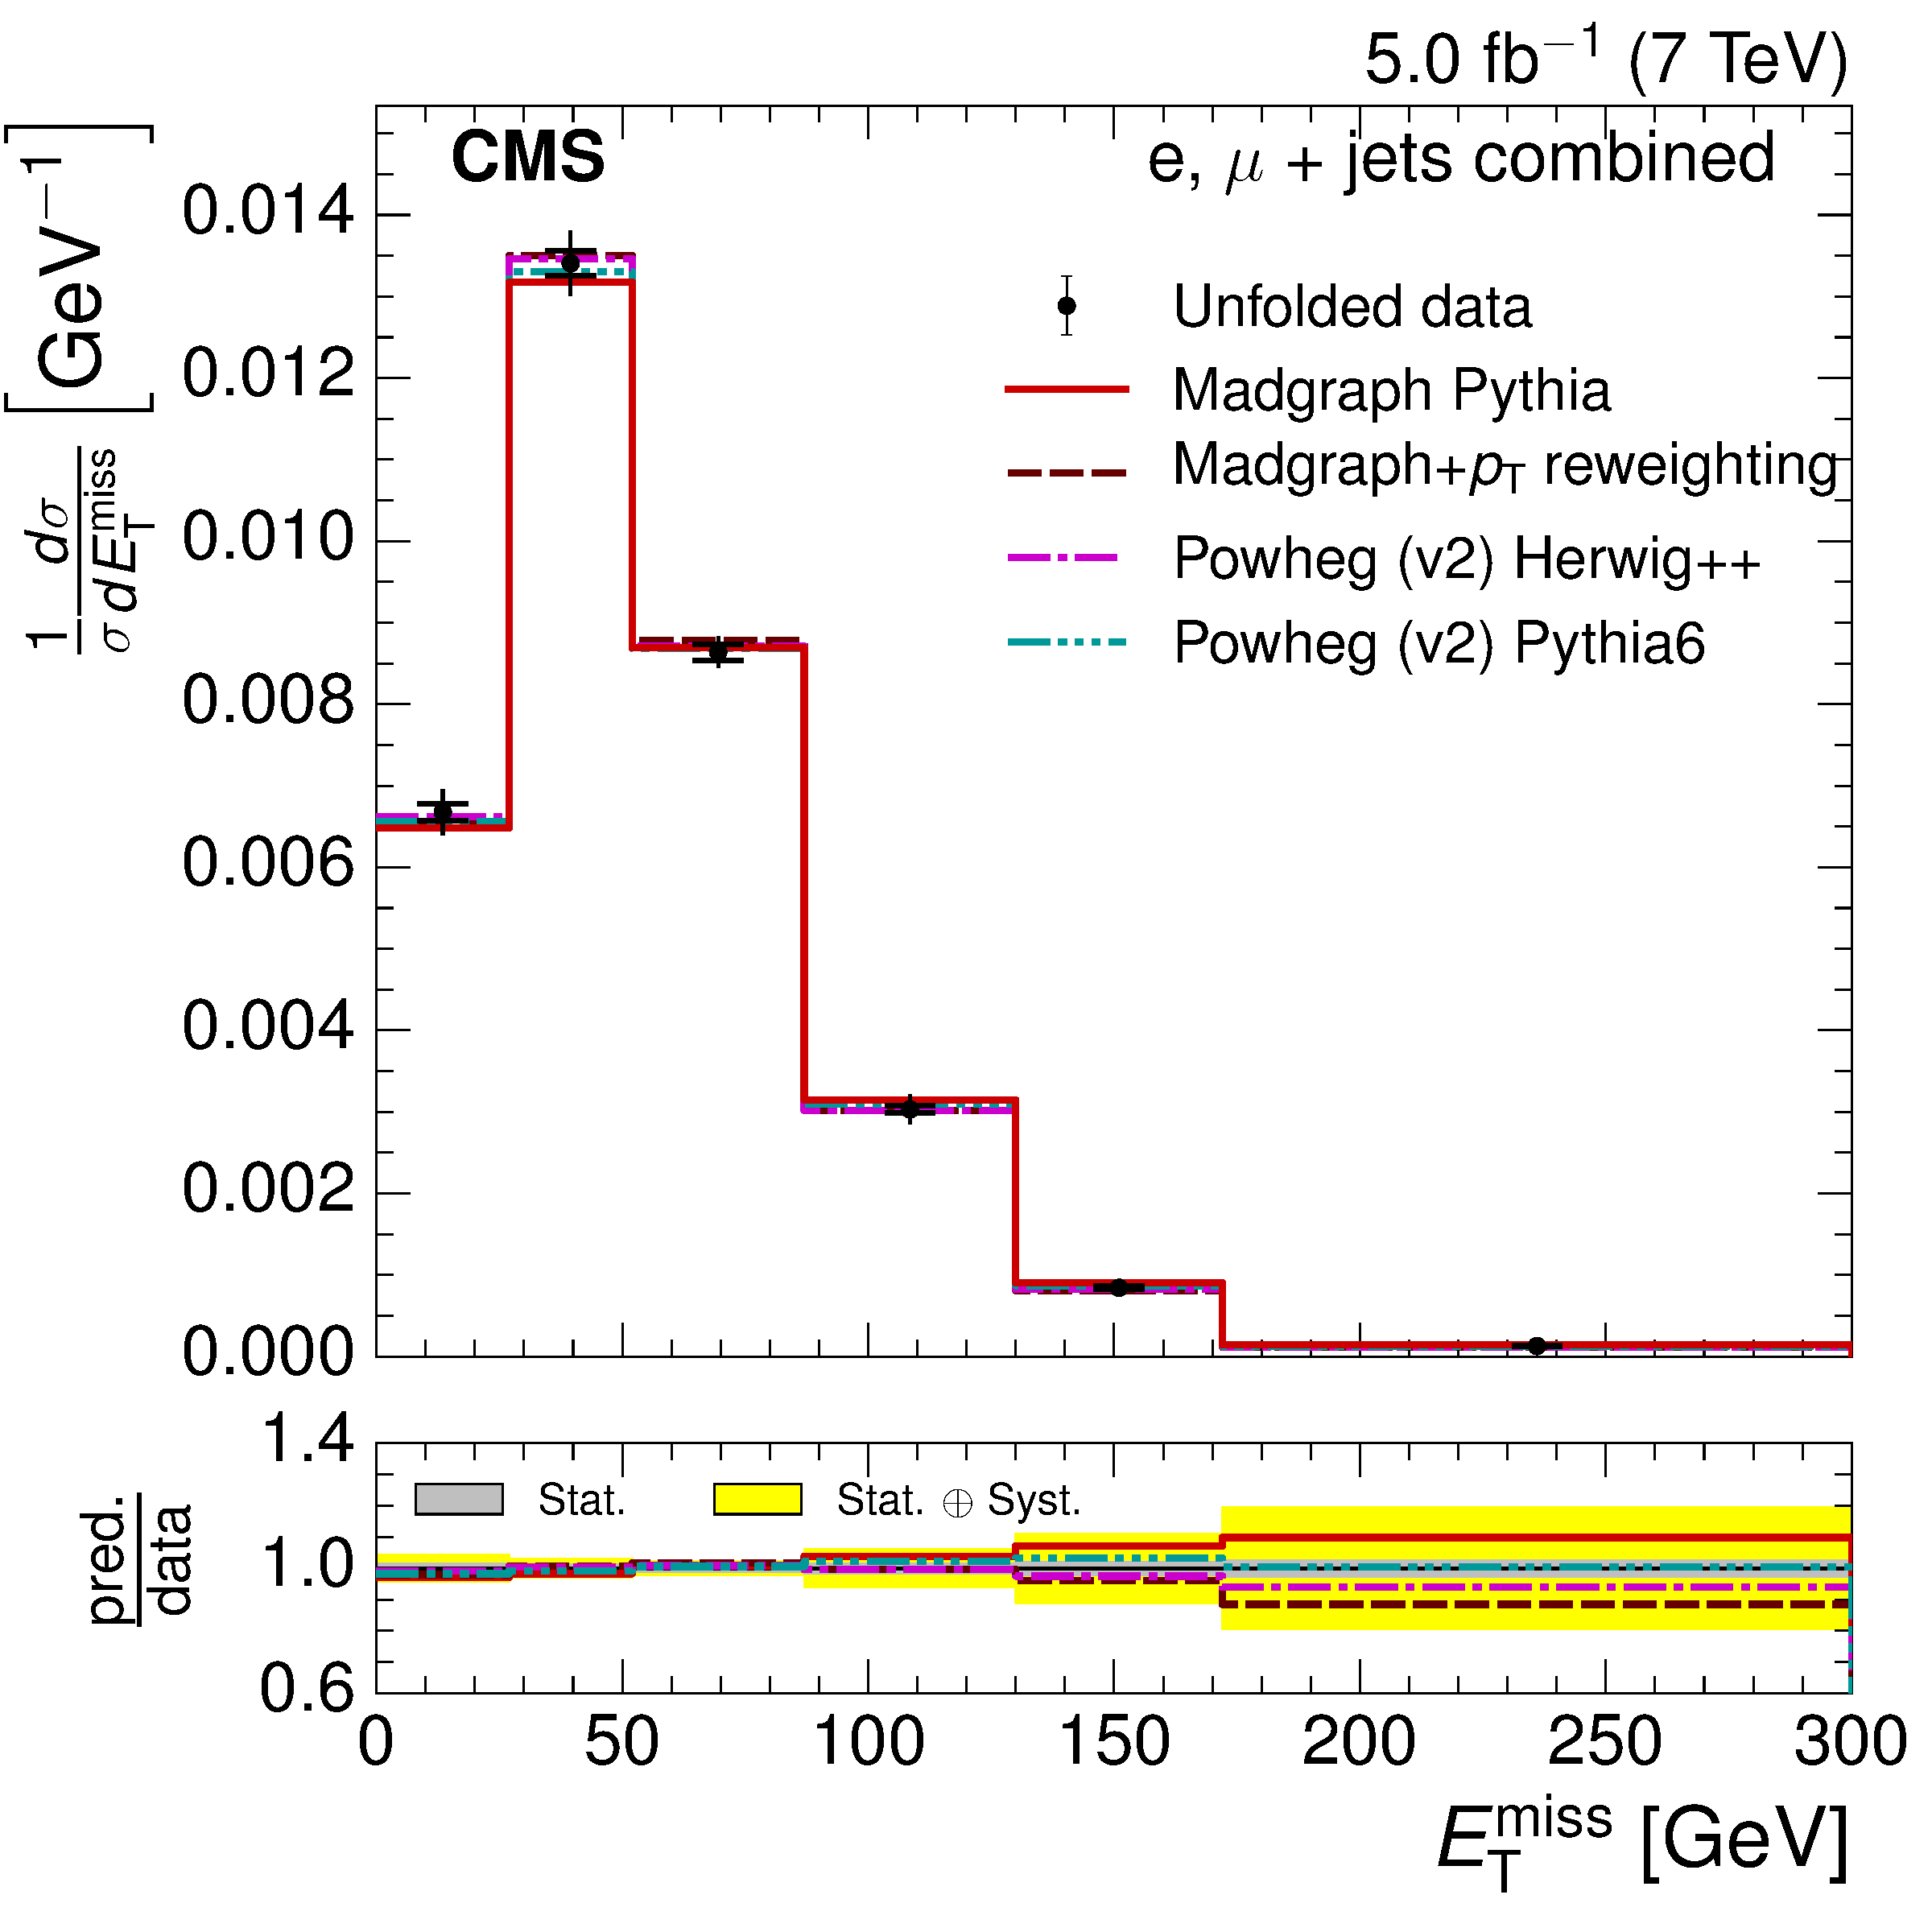
\includegraphics[width=0.435\textwidth]{Chapters/07_08_09_Analysis/Images/results/fit/7TeV/MET/central/normalised_xsection_combined_different_generators.pdf}\hfill
     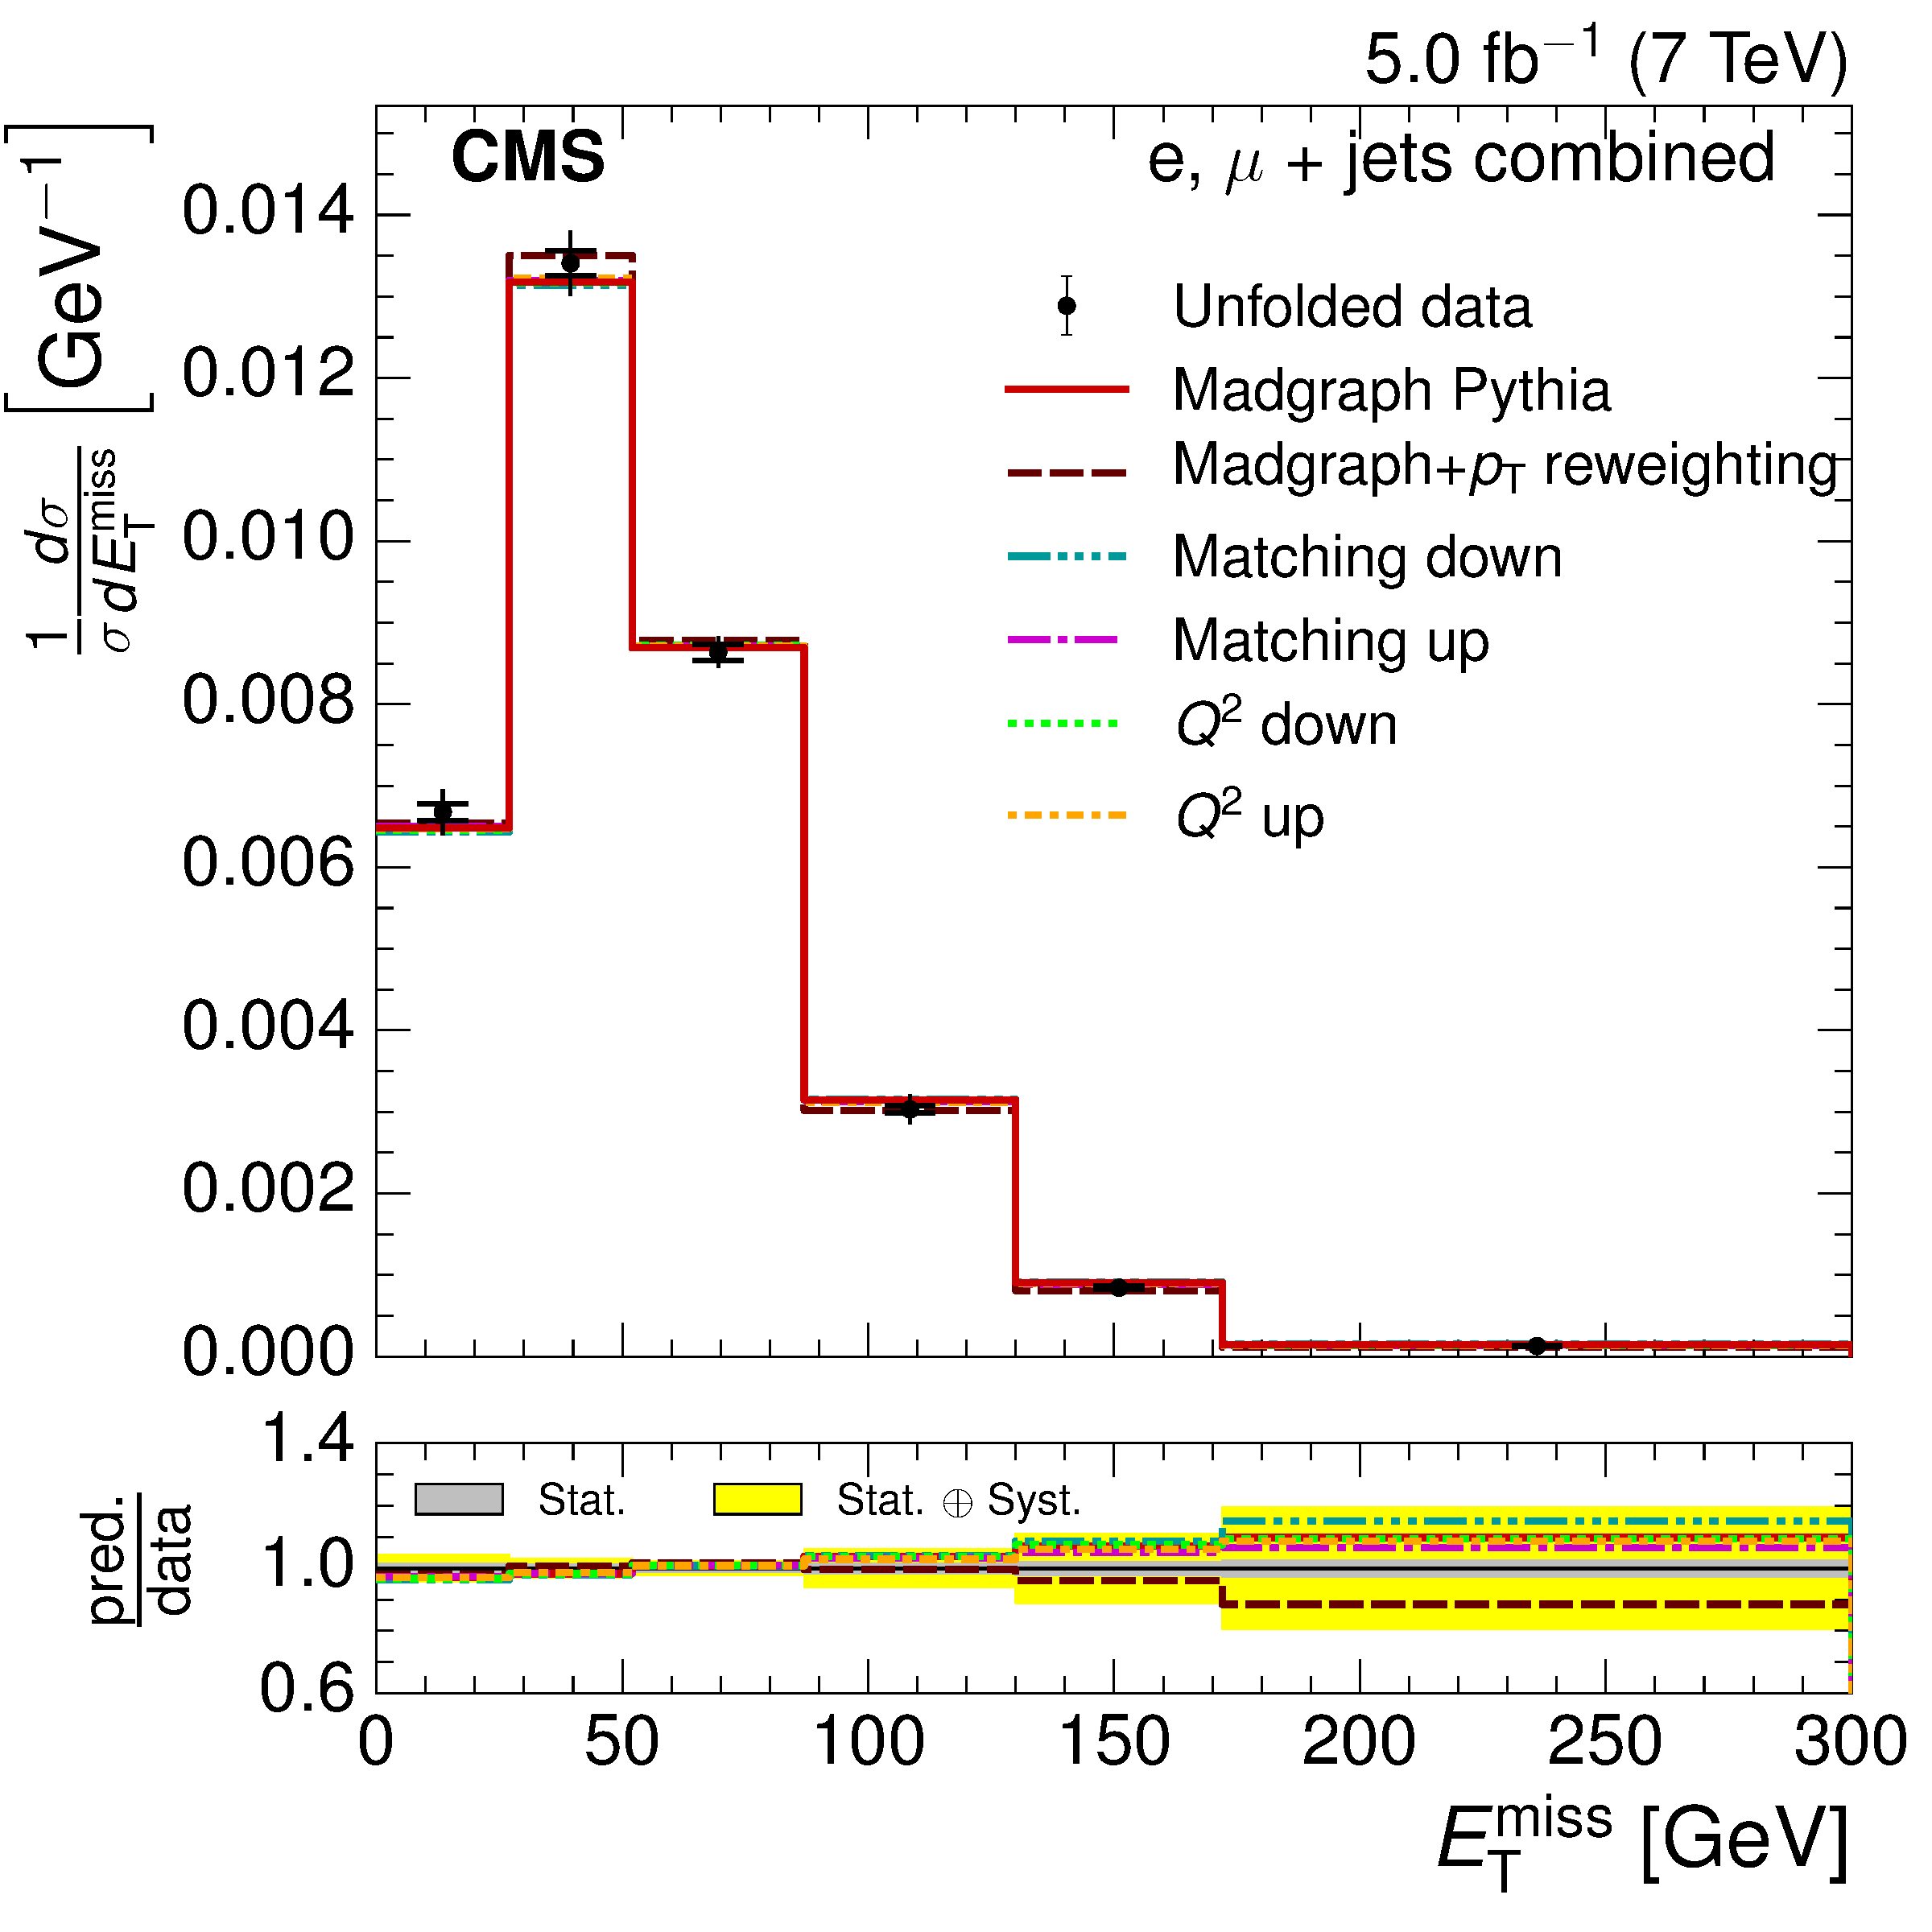
\includegraphics[width=0.435\textwidth]{Chapters/07_08_09_Analysis/Images/results/fit/7TeV/MET/central/normalised_xsection_combined_systematics_shifts.pdf}\\
     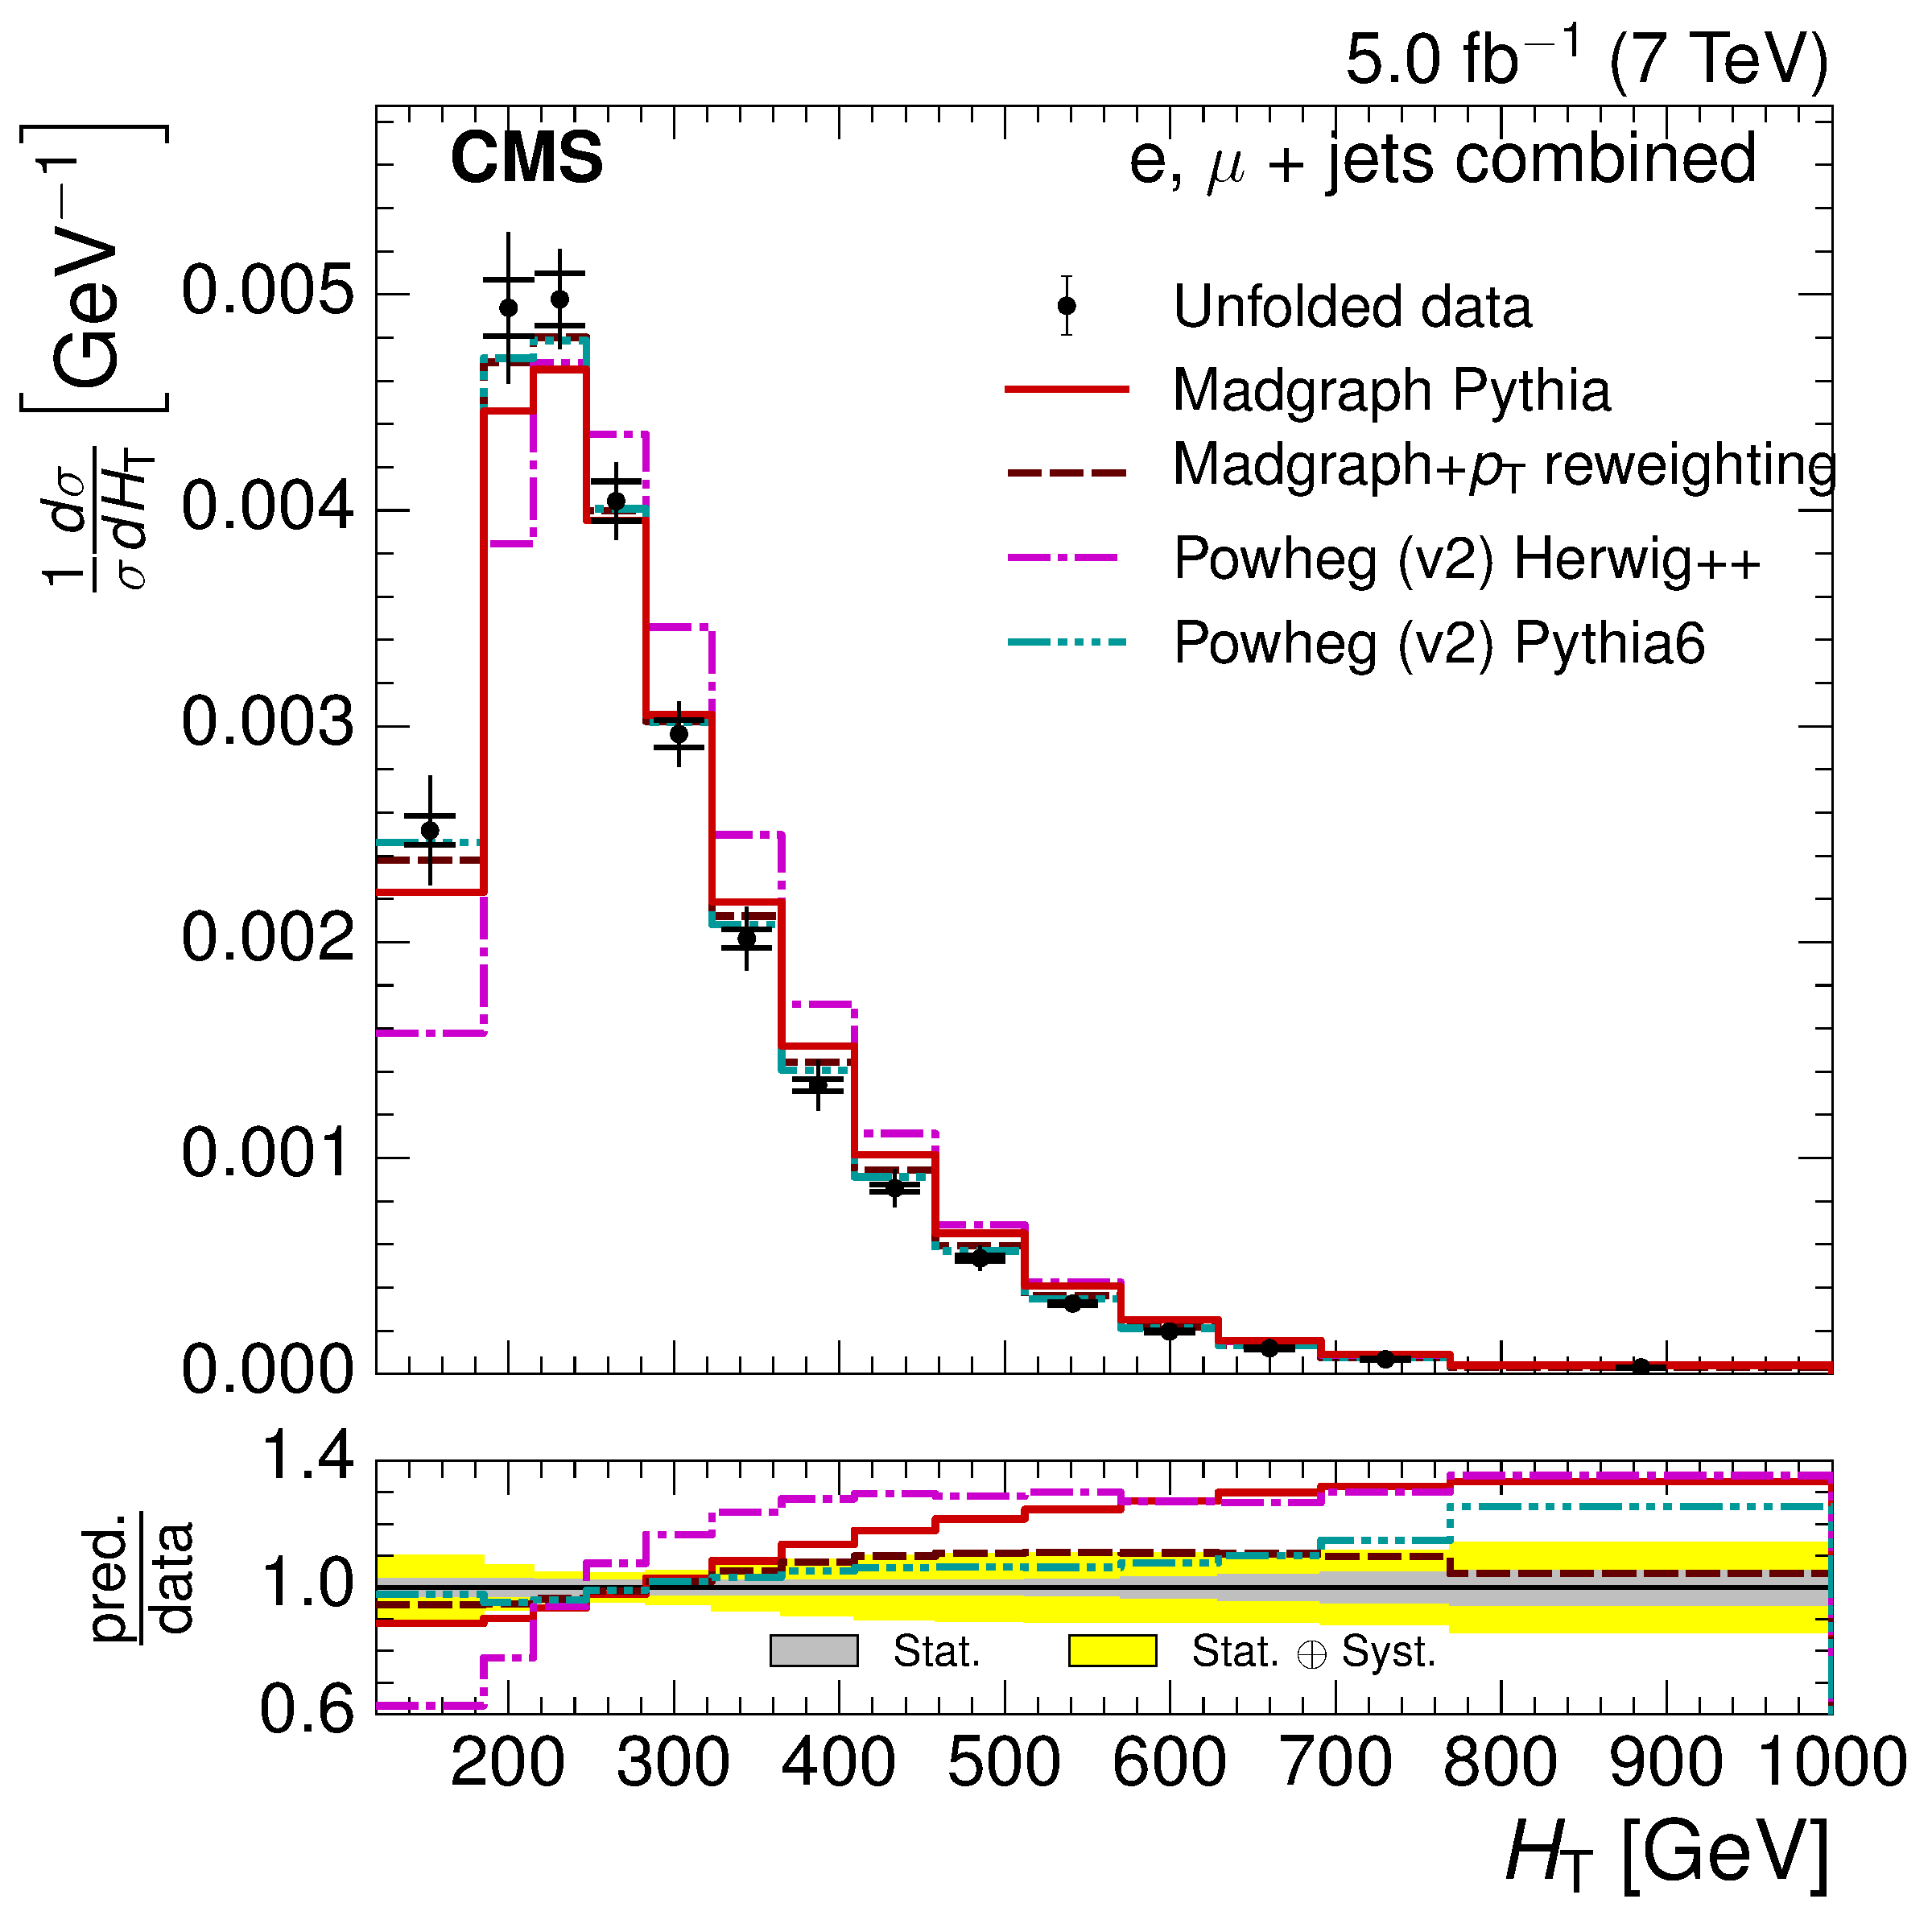
\includegraphics[width=0.435\textwidth]{Chapters/07_08_09_Analysis/Images/results/fit/7TeV/HT/central/normalised_xsection_combined_different_generators.pdf}\hfill
     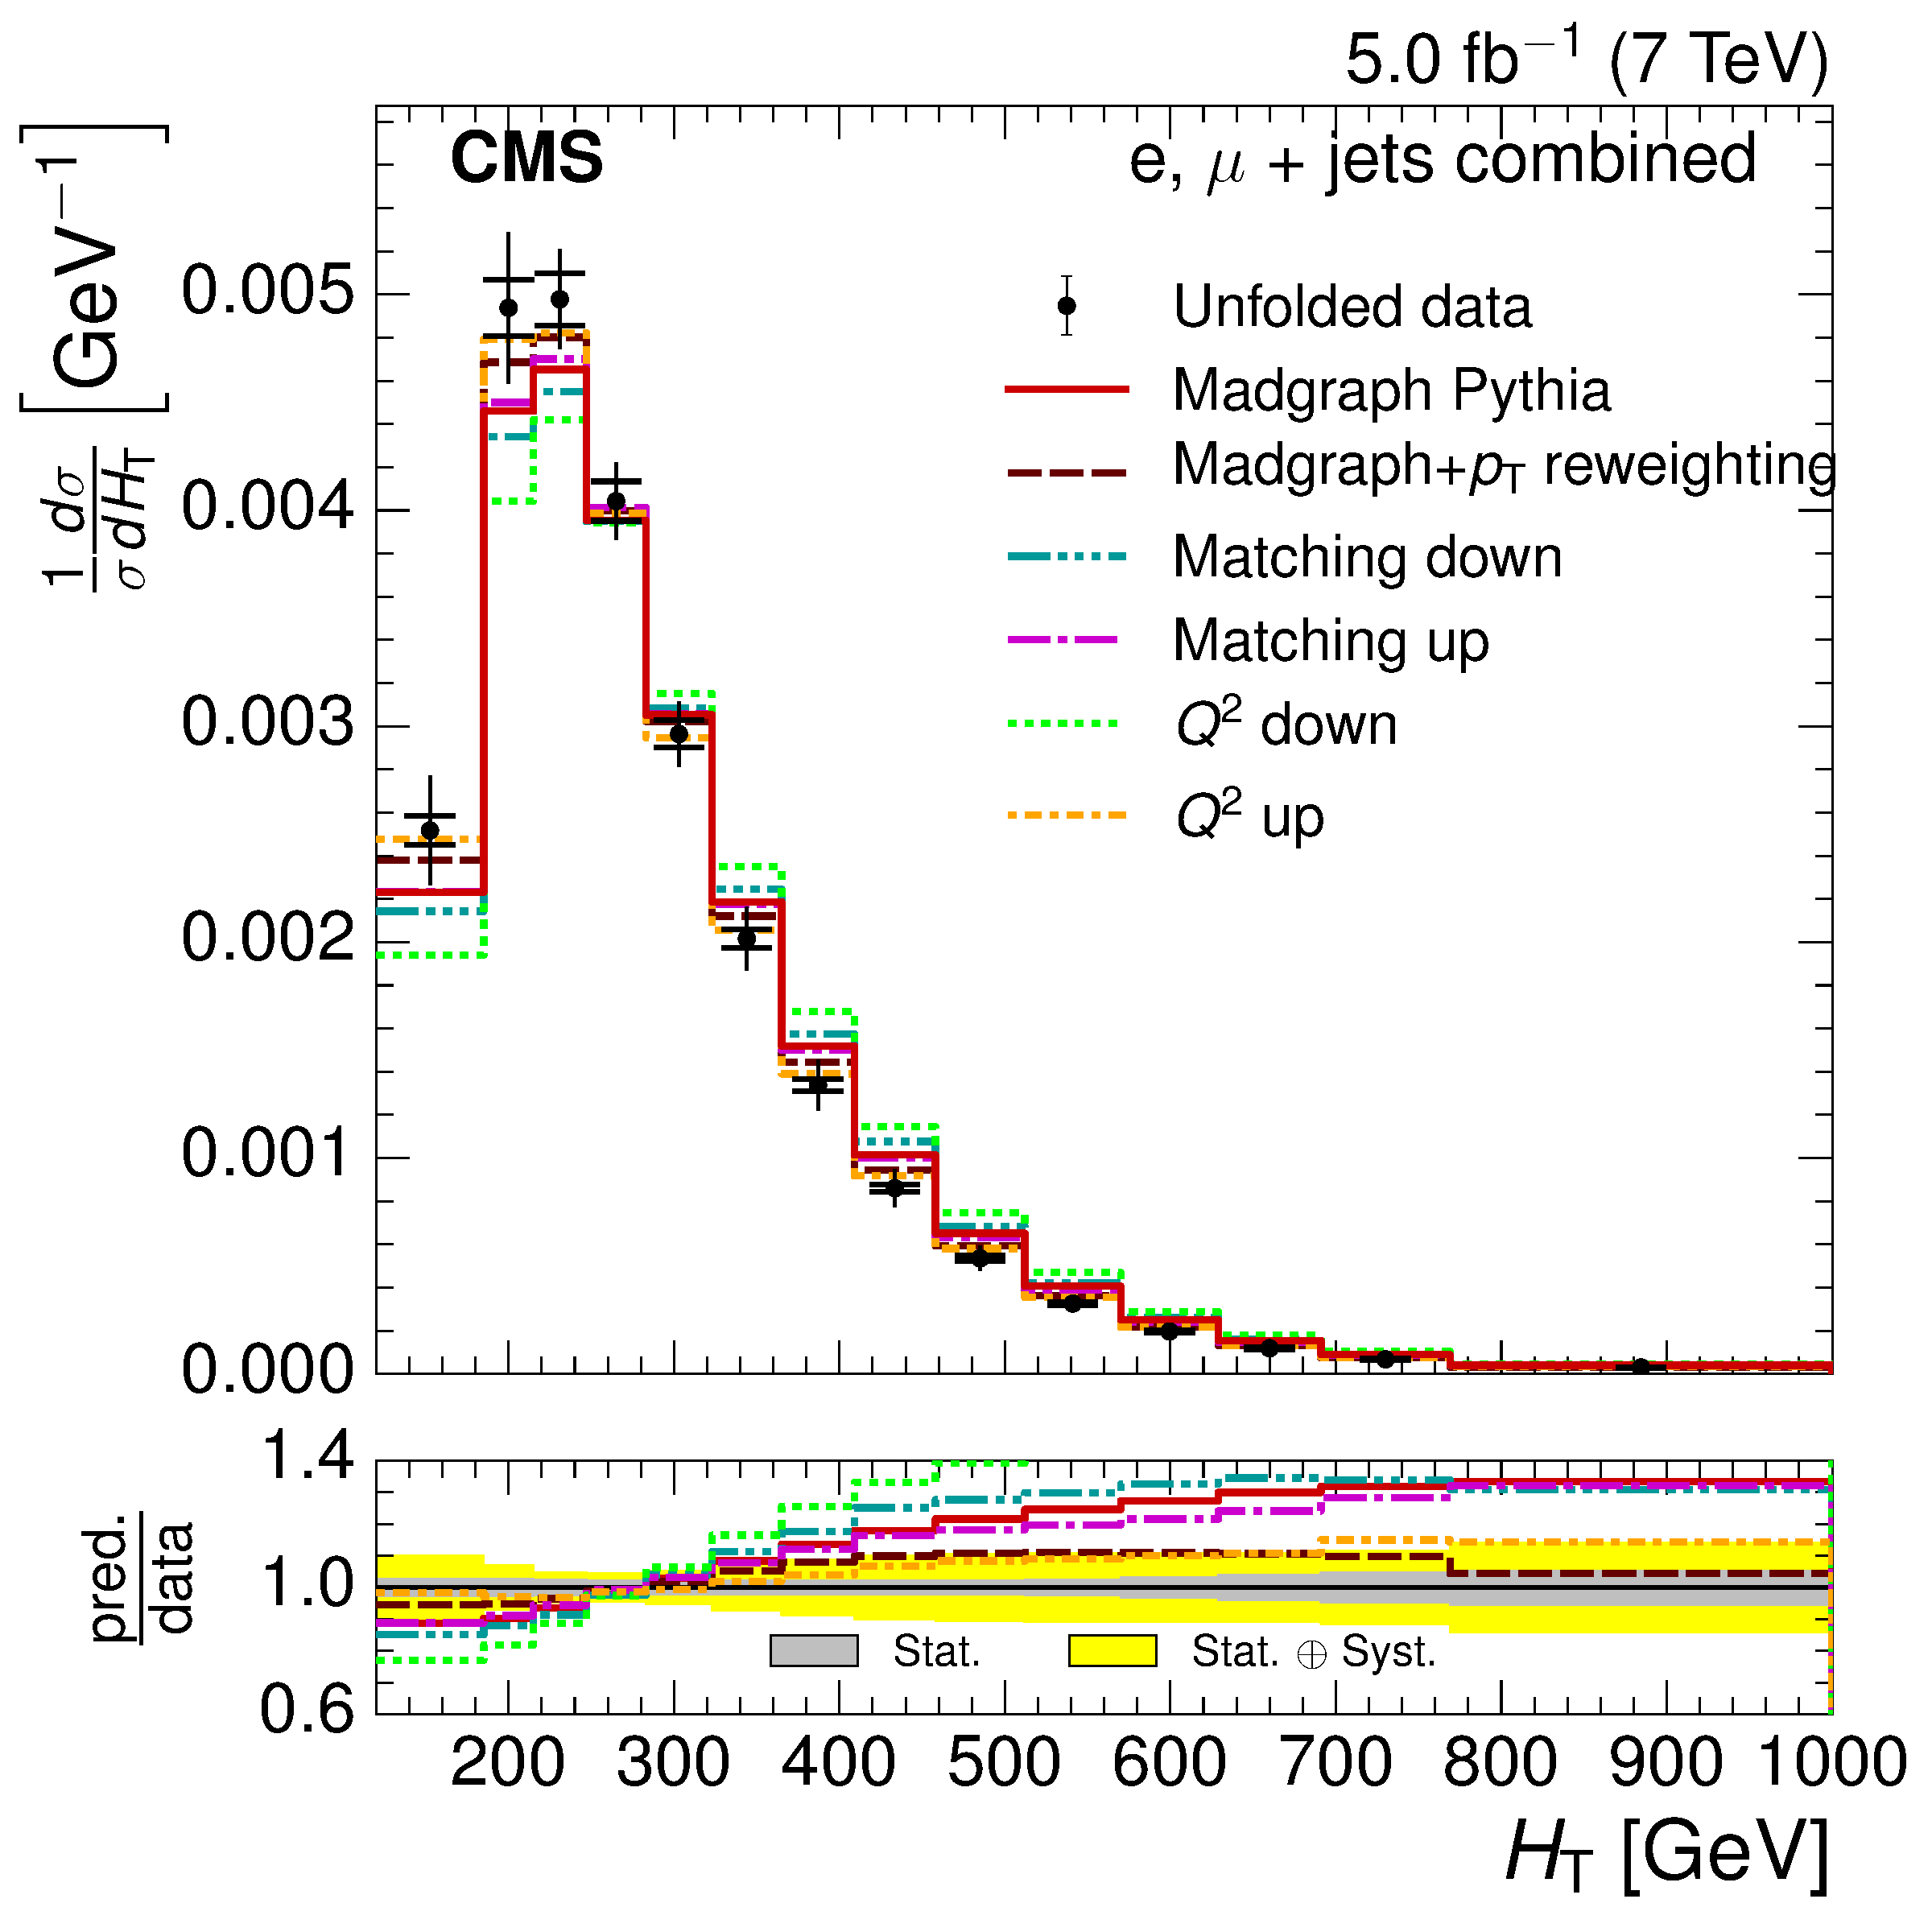
\includegraphics[width=0.435\textwidth]{Chapters/07_08_09_Analysis/Images/results/fit/7TeV/HT/central/normalised_xsection_combined_systematics_shifts.pdf}\\
     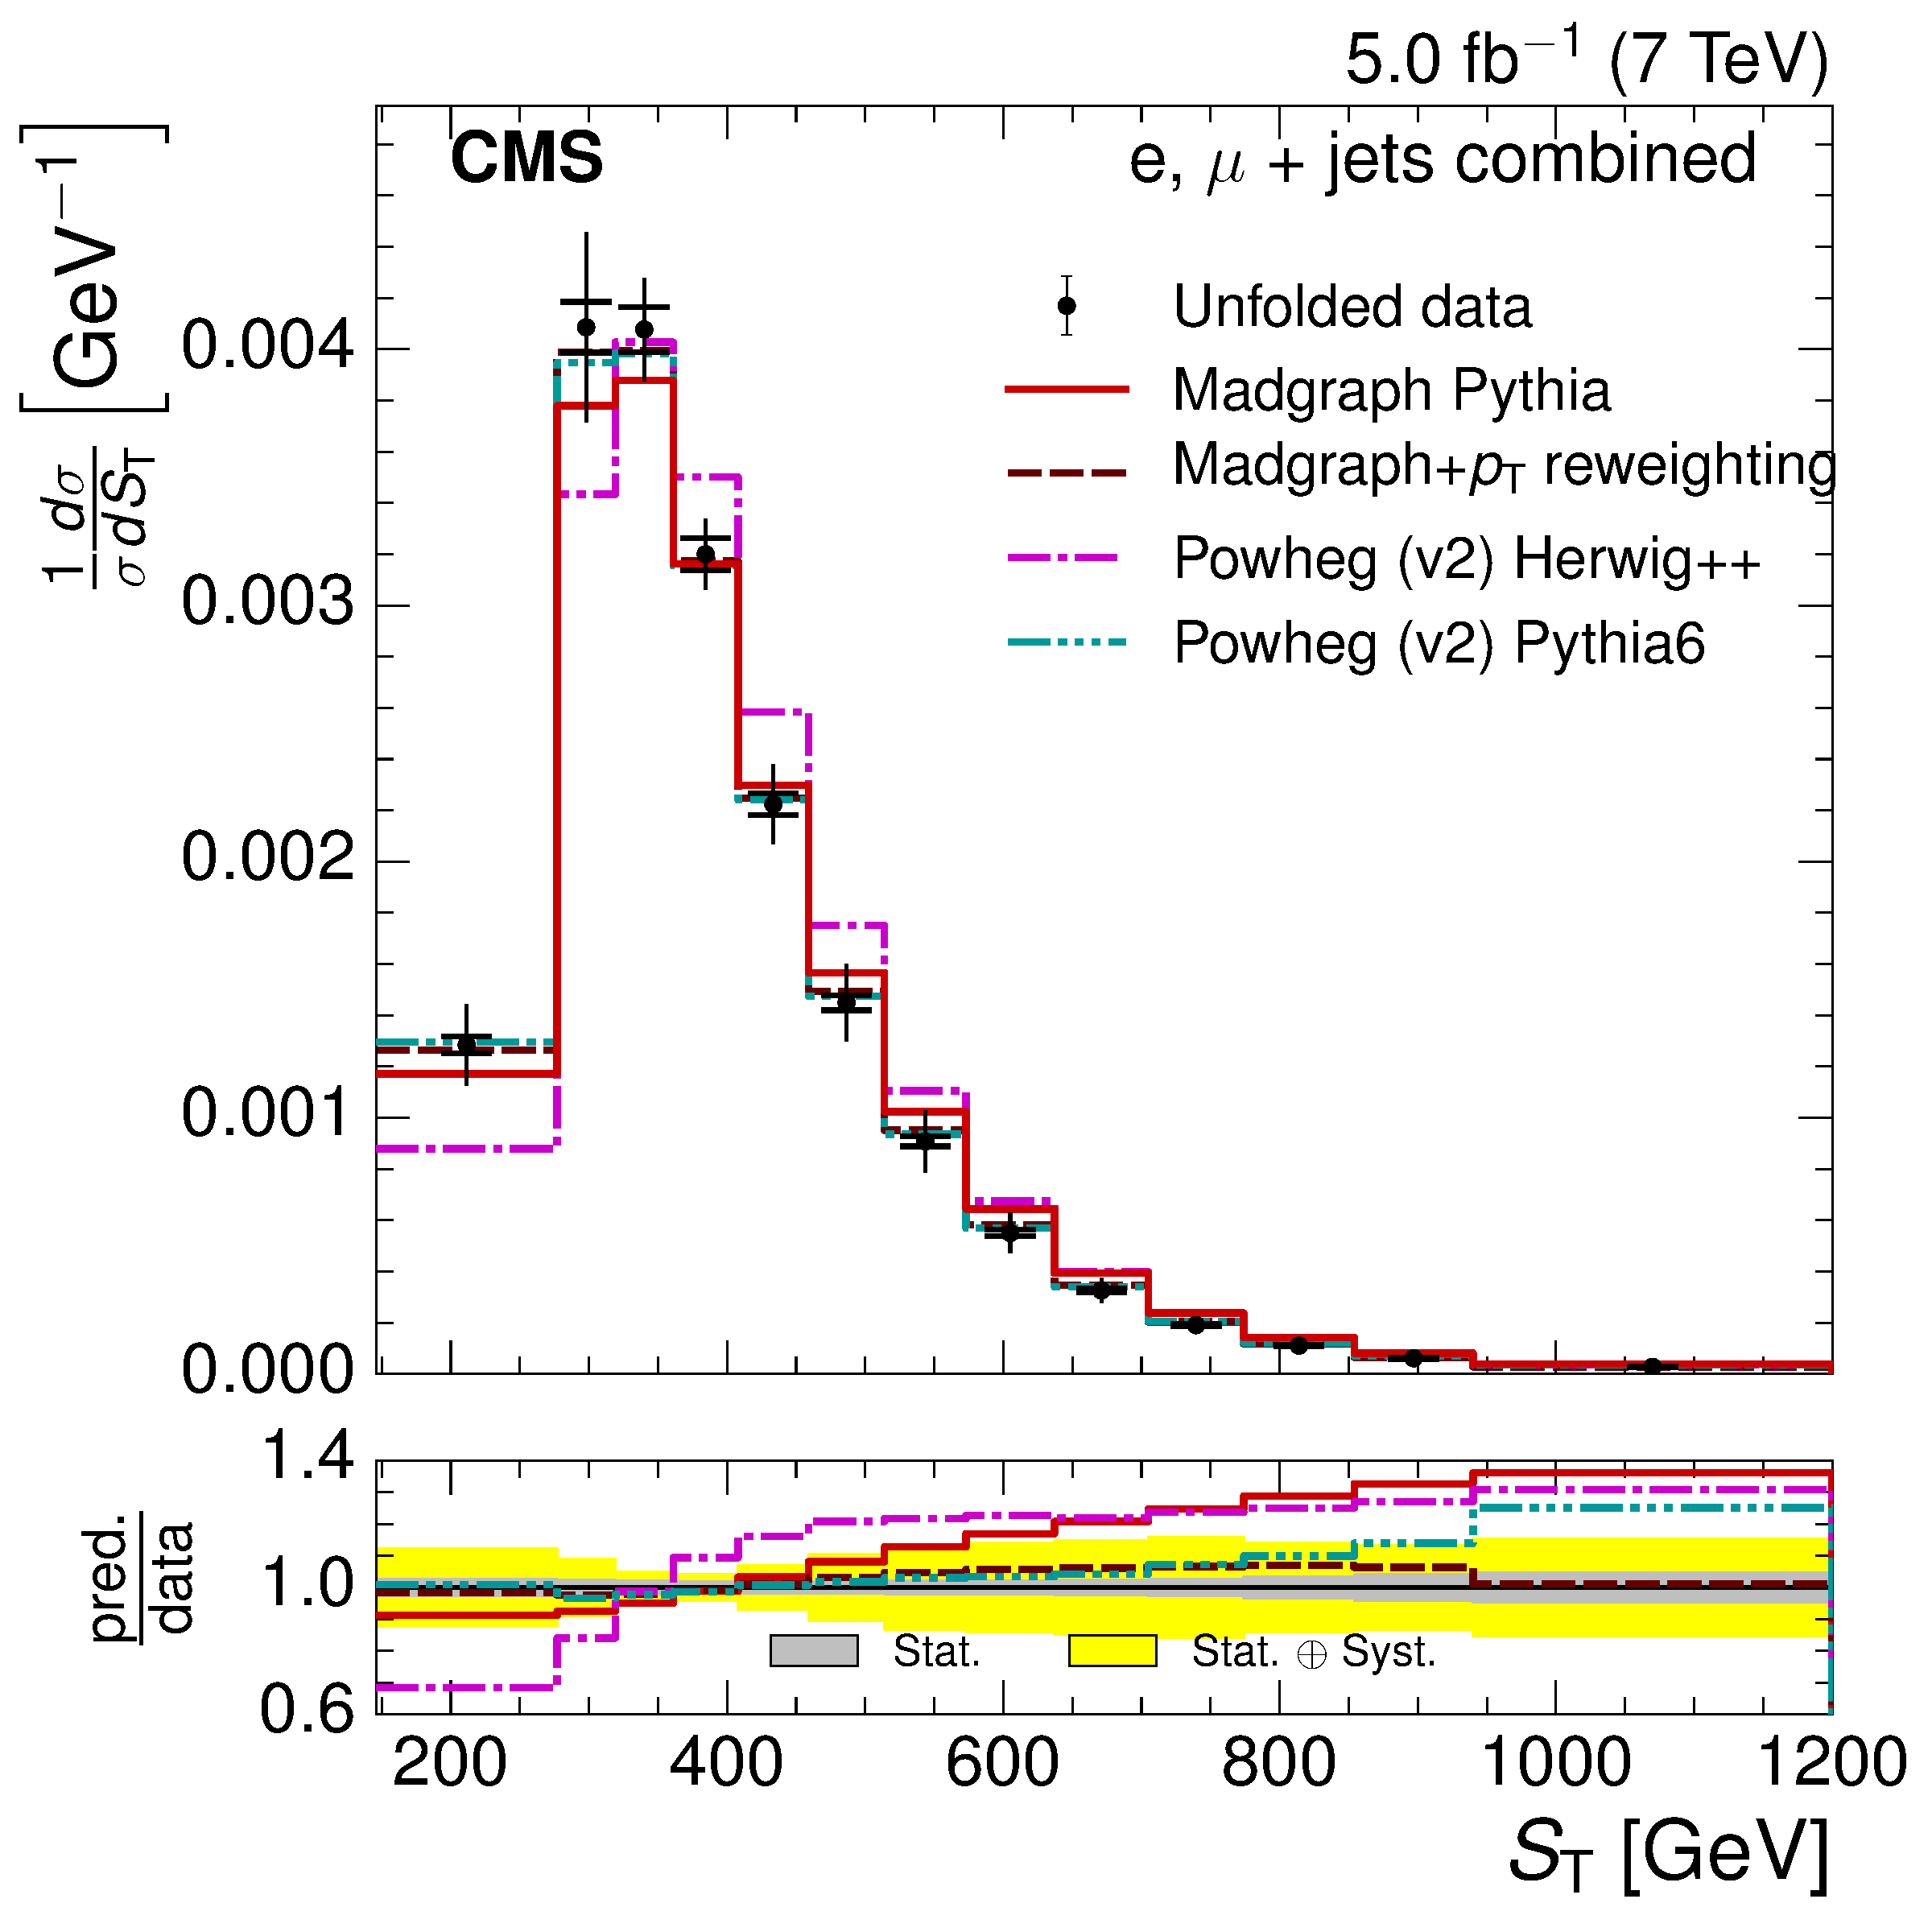
\includegraphics[width=0.435\textwidth]{Chapters/07_08_09_Analysis/Images/results/fit/7TeV/ST/central/normalised_xsection_combined_different_generators.pdf}\hfill
     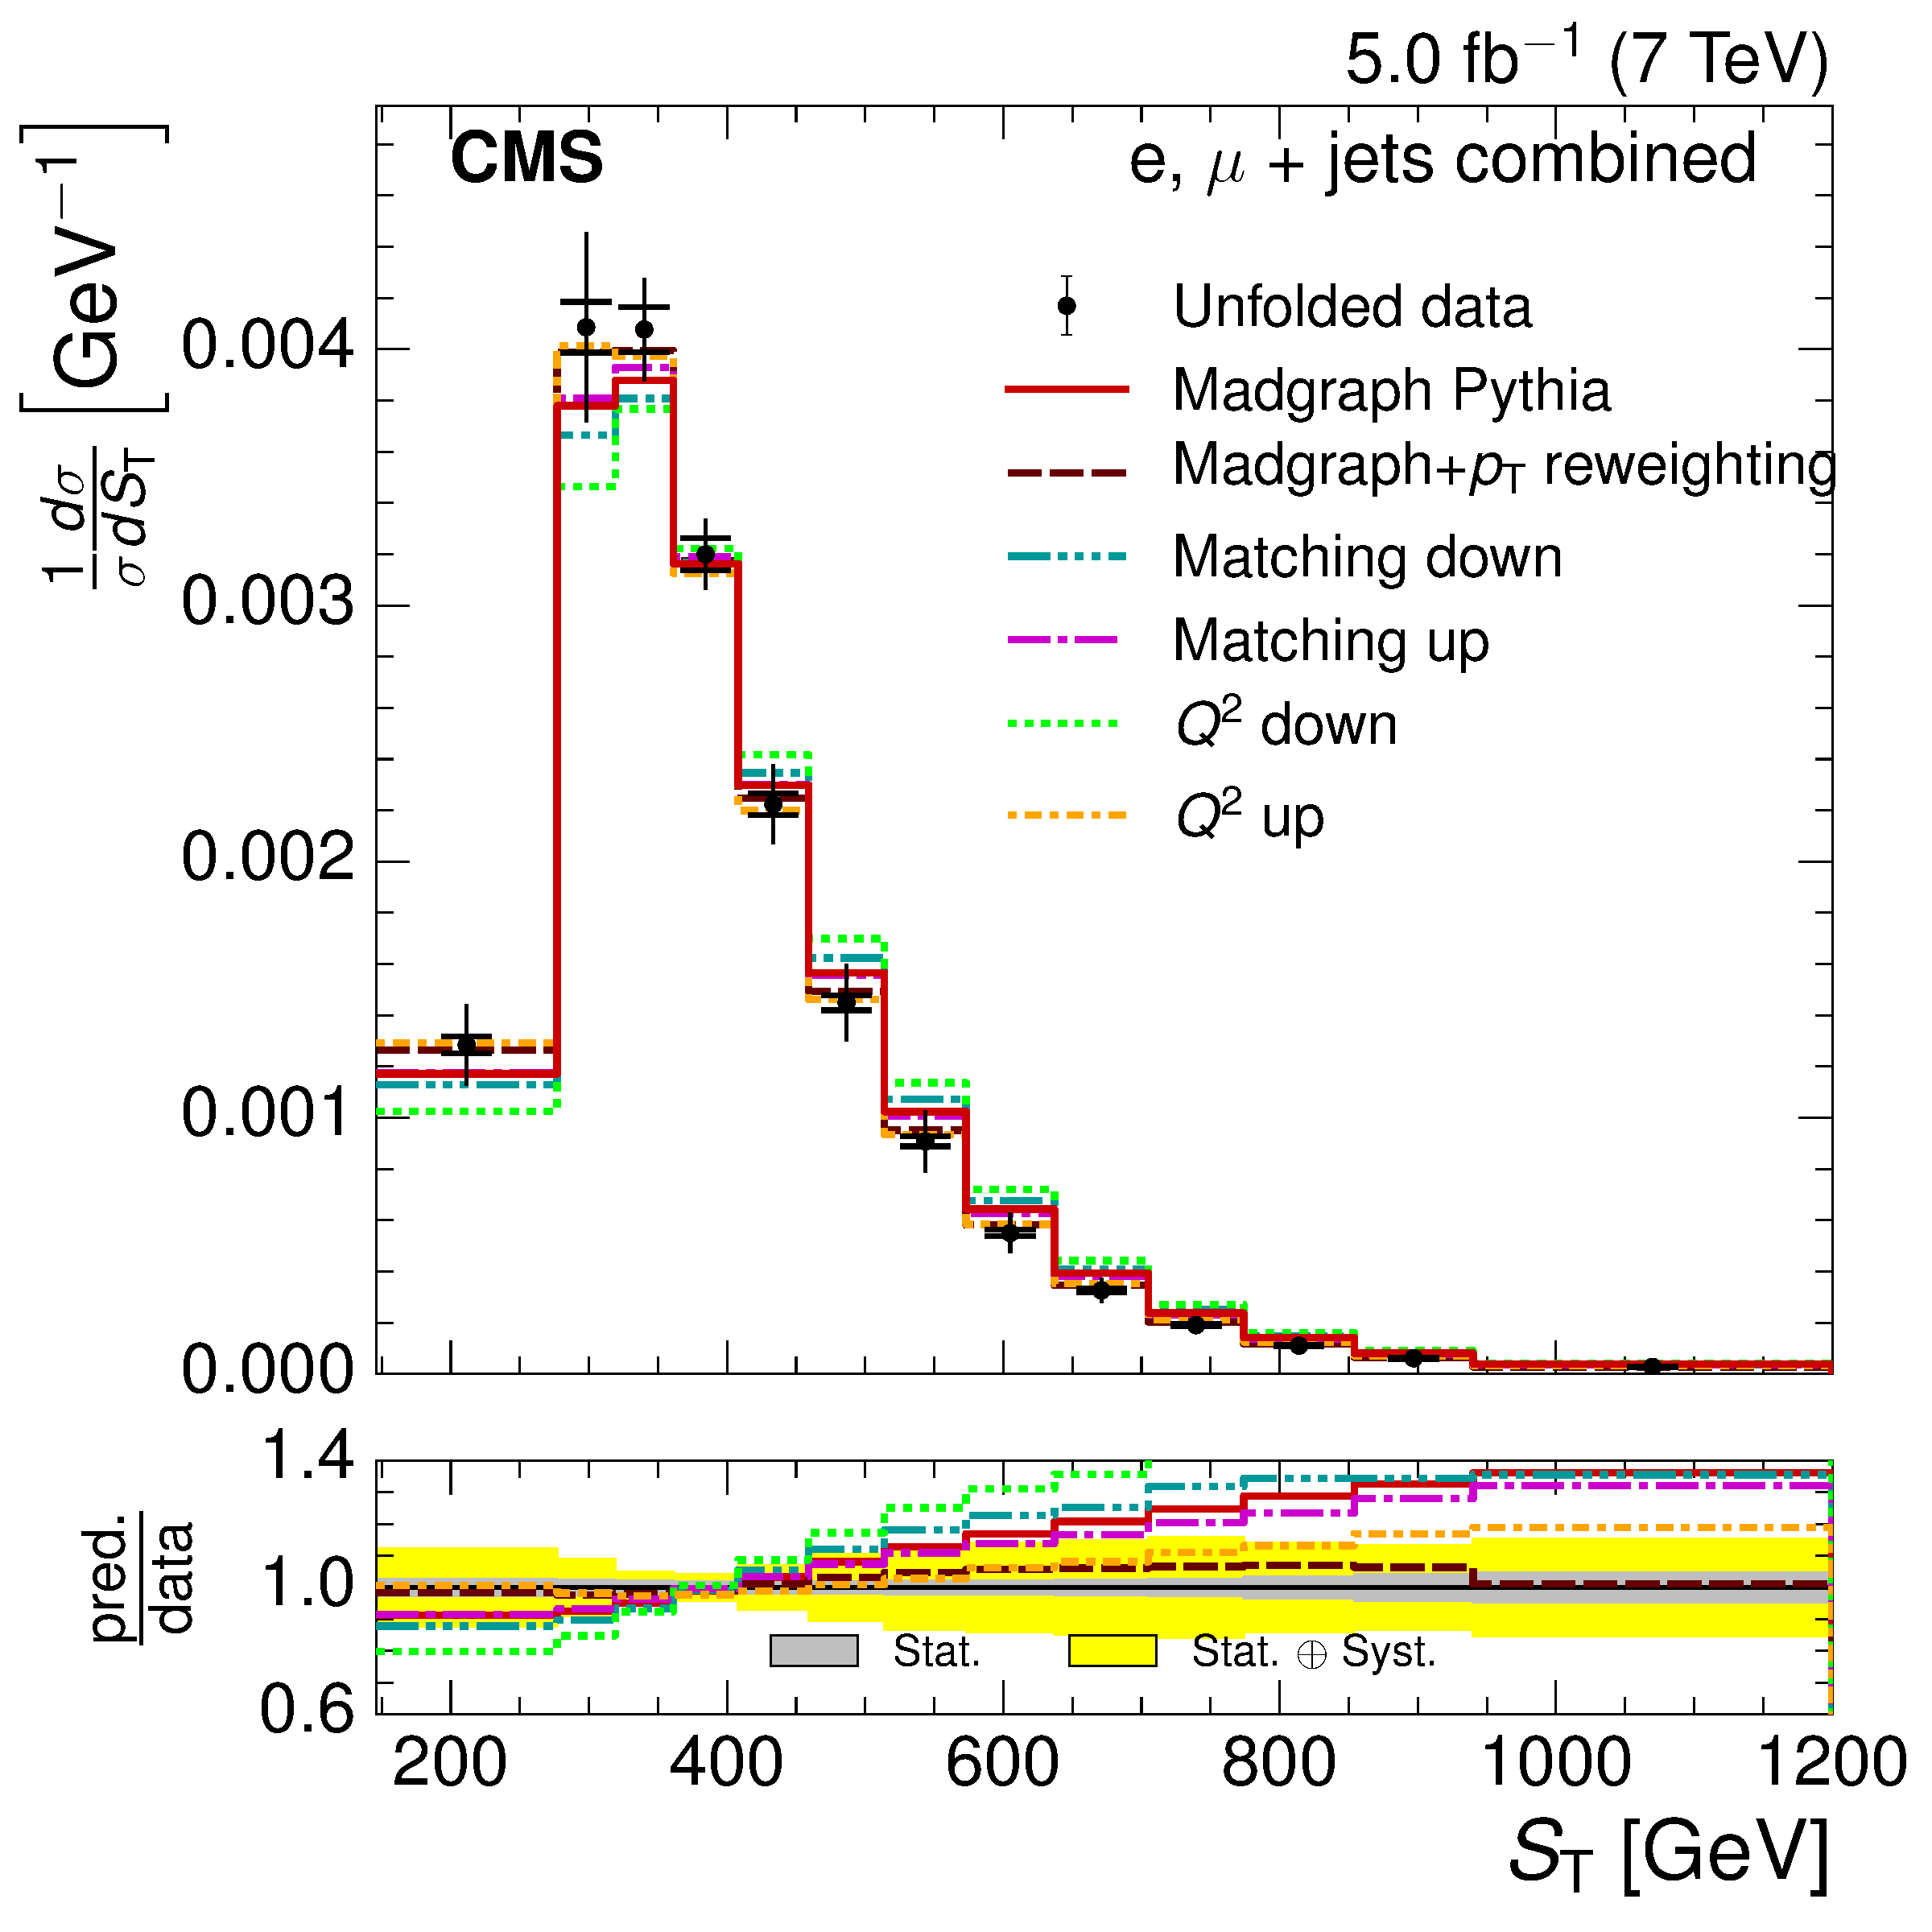
\includegraphics[width=0.435\textwidth]{Chapters/07_08_09_Analysis/Images/results/fit/7TeV/ST/central/normalised_xsection_combined_systematics_shifts.pdf}\\
     \caption[Comparison of the measured normalised differential cross section with respect to \met, \HT and
     \st to different Monte Carlo generators and predictions at $\roots=7\TeV$.]{Comparison of the measured
     normalised differential cross section with respect to \met (upper), \HT (middle) and \st (lower) to
     different Monte Carlo generators: \MADGRAPH, \POWHEGHERWIG2, \POWHEGPYTHIA2 and \MADGRAPH corrected for
     top \pt mismodelling (left) and to different Monte Carlo predictions matching threshold up/down and
     factorisation scale up/down (right) in the combined electron+jets and muon+jets channel at
     $\roots=7\TeV$. The lower plots show the ratio of the predictions to the data.}     
     \label{fig:result_MET_HT_ST_7TeV_combined}
\end{figure}

\begin{figure}[hbtp]
    \centering
     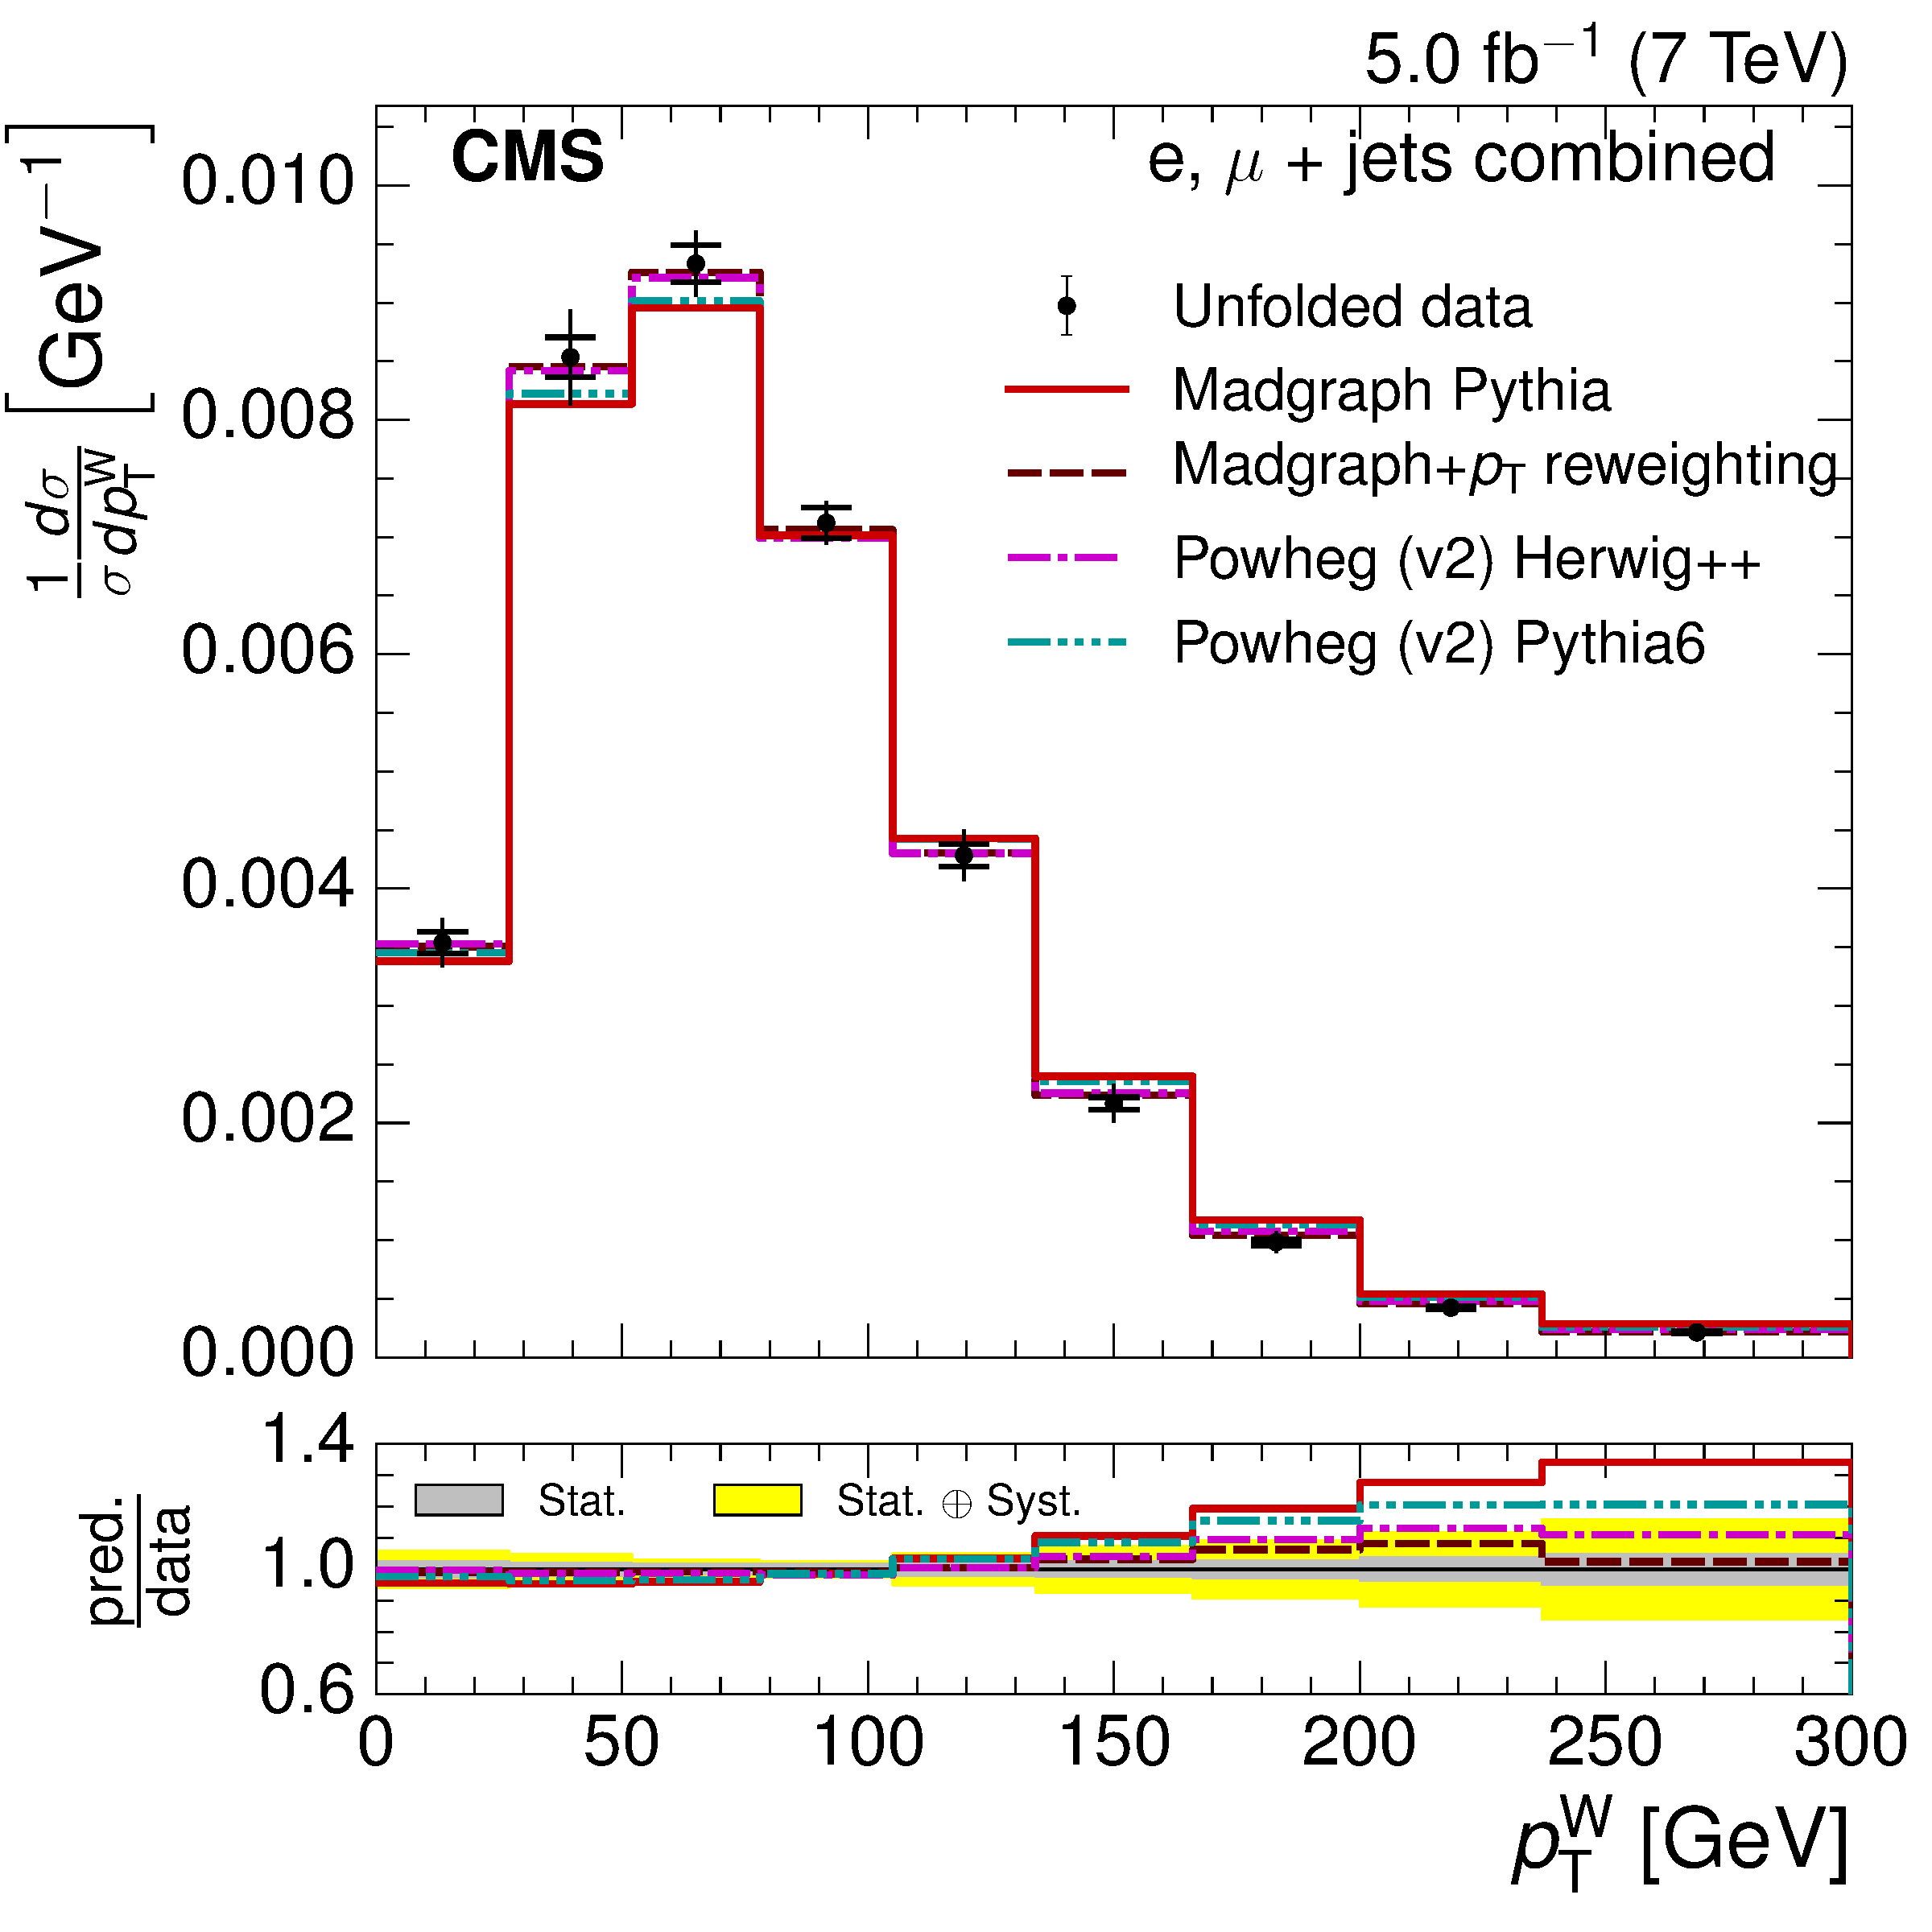
\includegraphics[width=0.48\textwidth]{Chapters/07_08_09_Analysis/Images/results/fit/7TeV/WPT/central/normalised_xsection_combined_different_generators.pdf}\hfill
     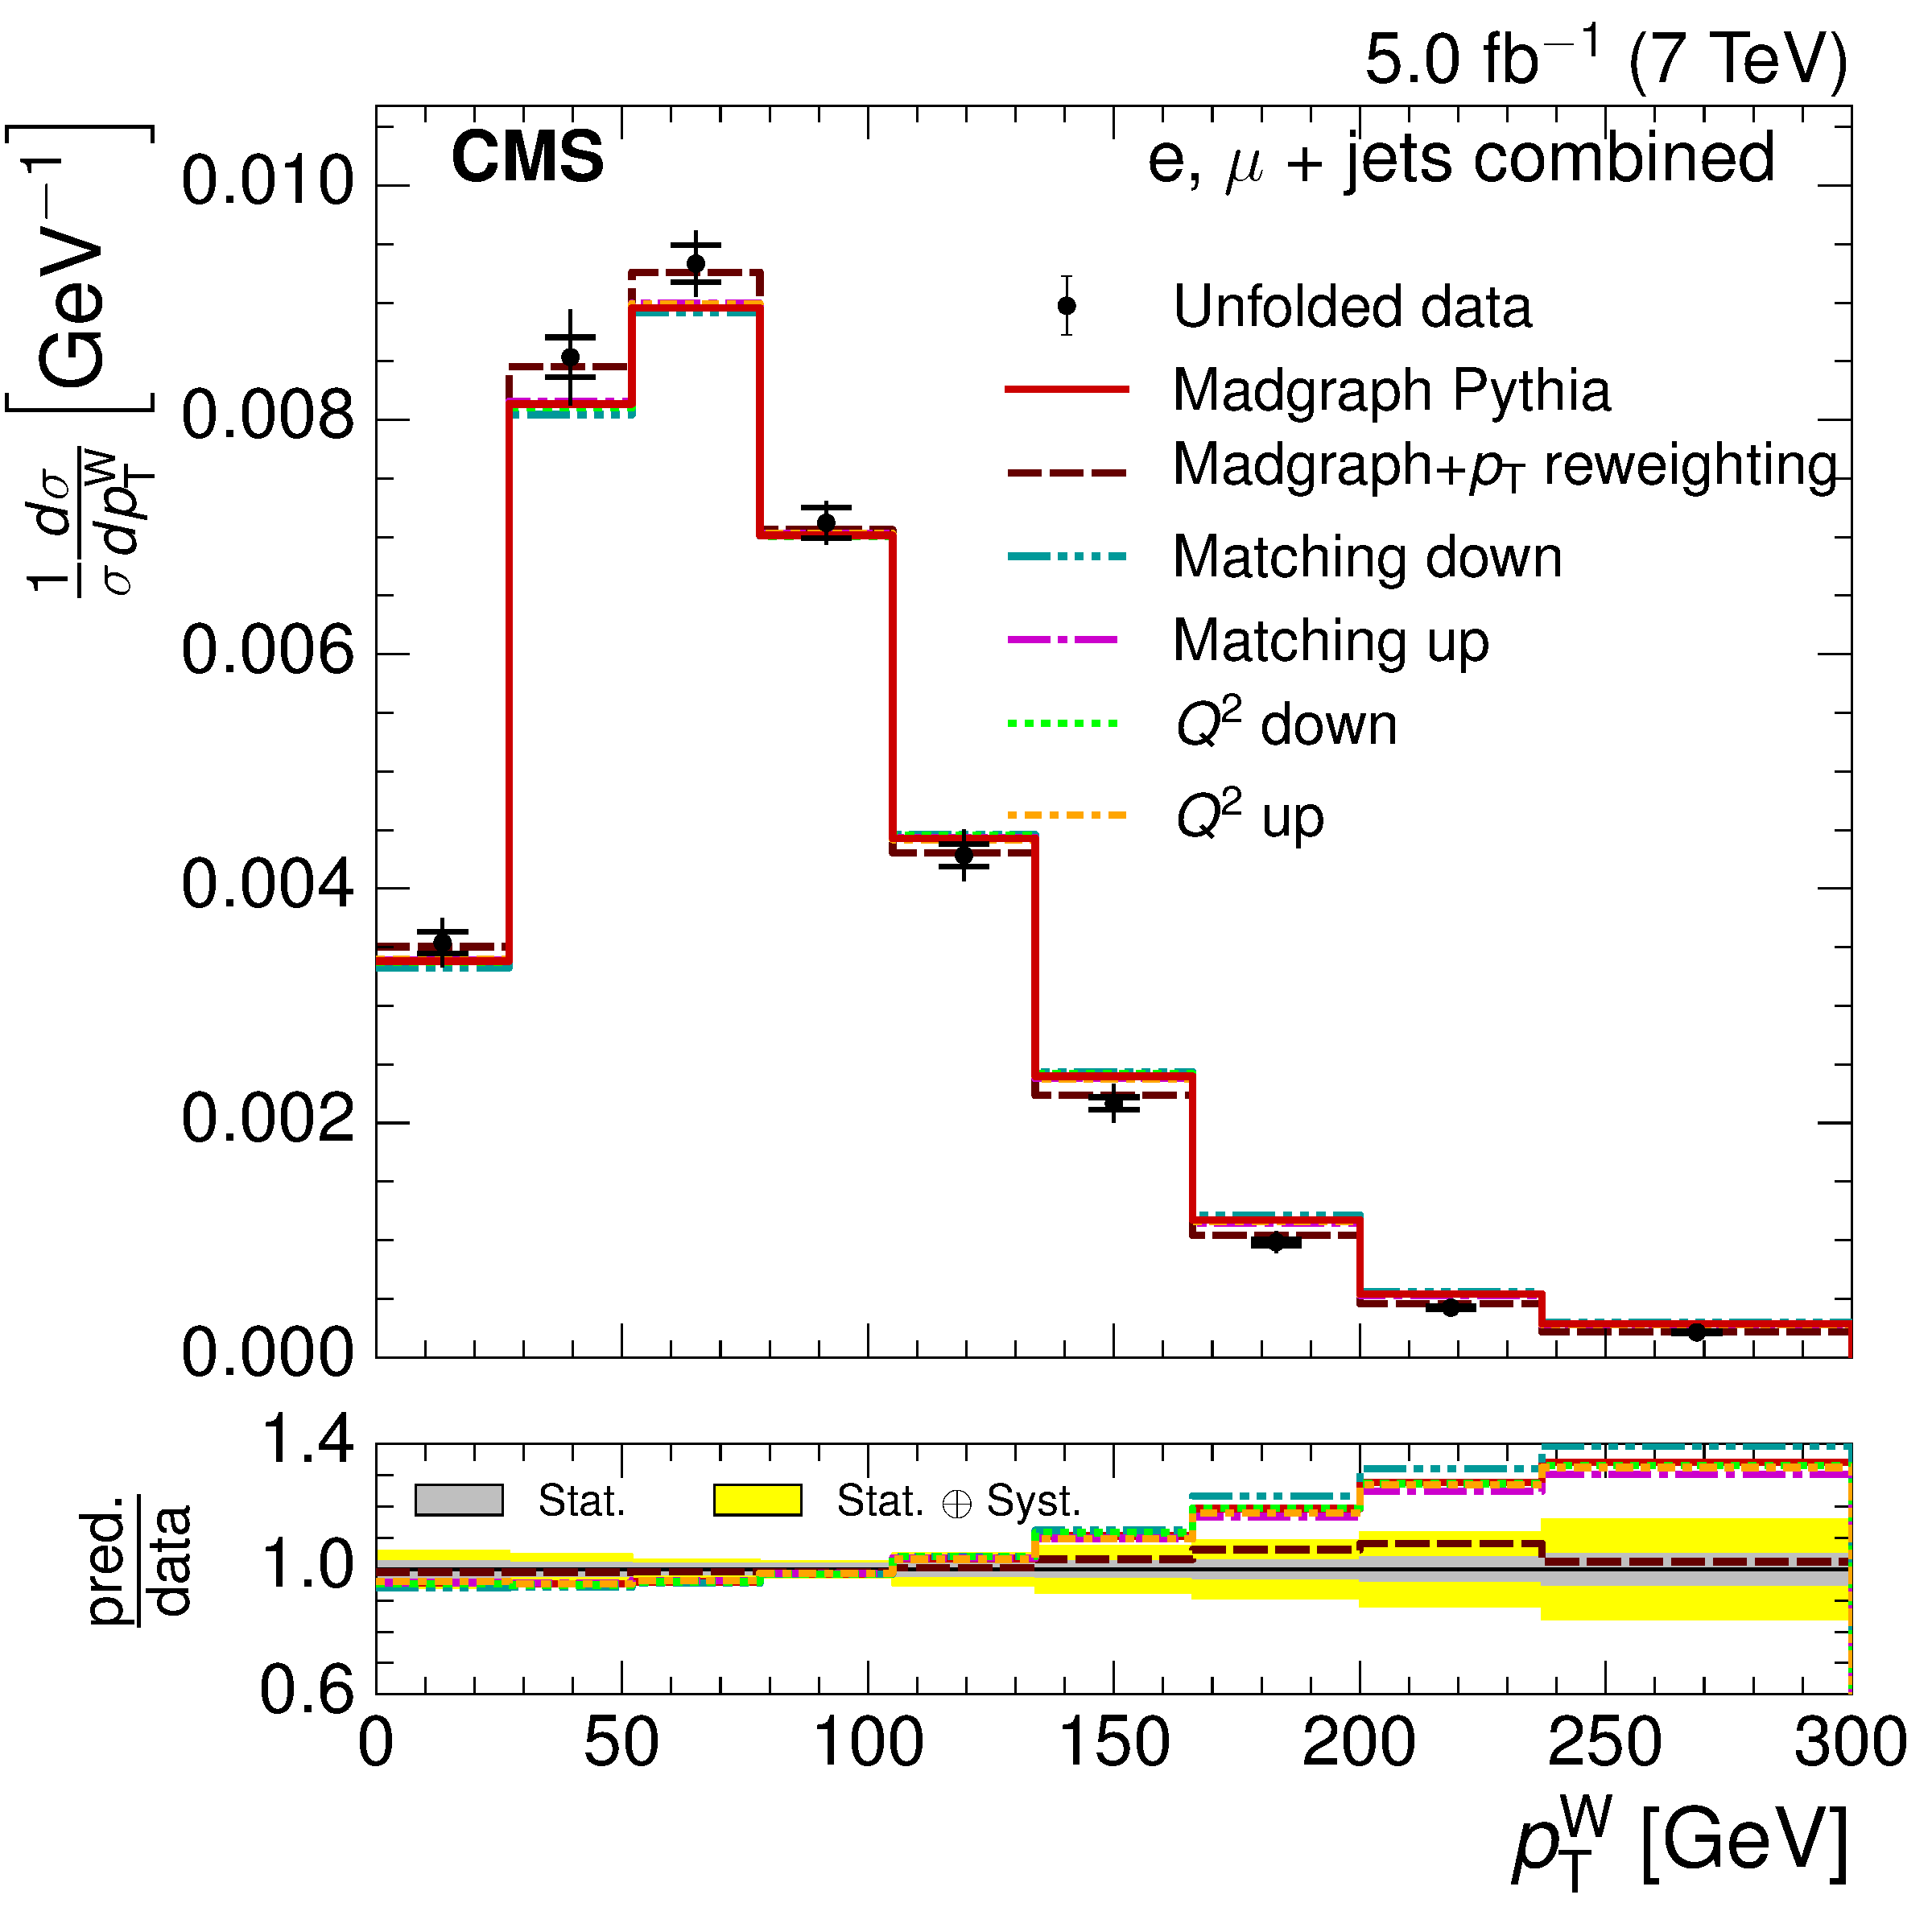
\includegraphics[width=0.48\textwidth]{Chapters/07_08_09_Analysis/Images/results/fit/7TeV/WPT/central/normalised_xsection_combined_systematics_shifts.pdf}\hfill
     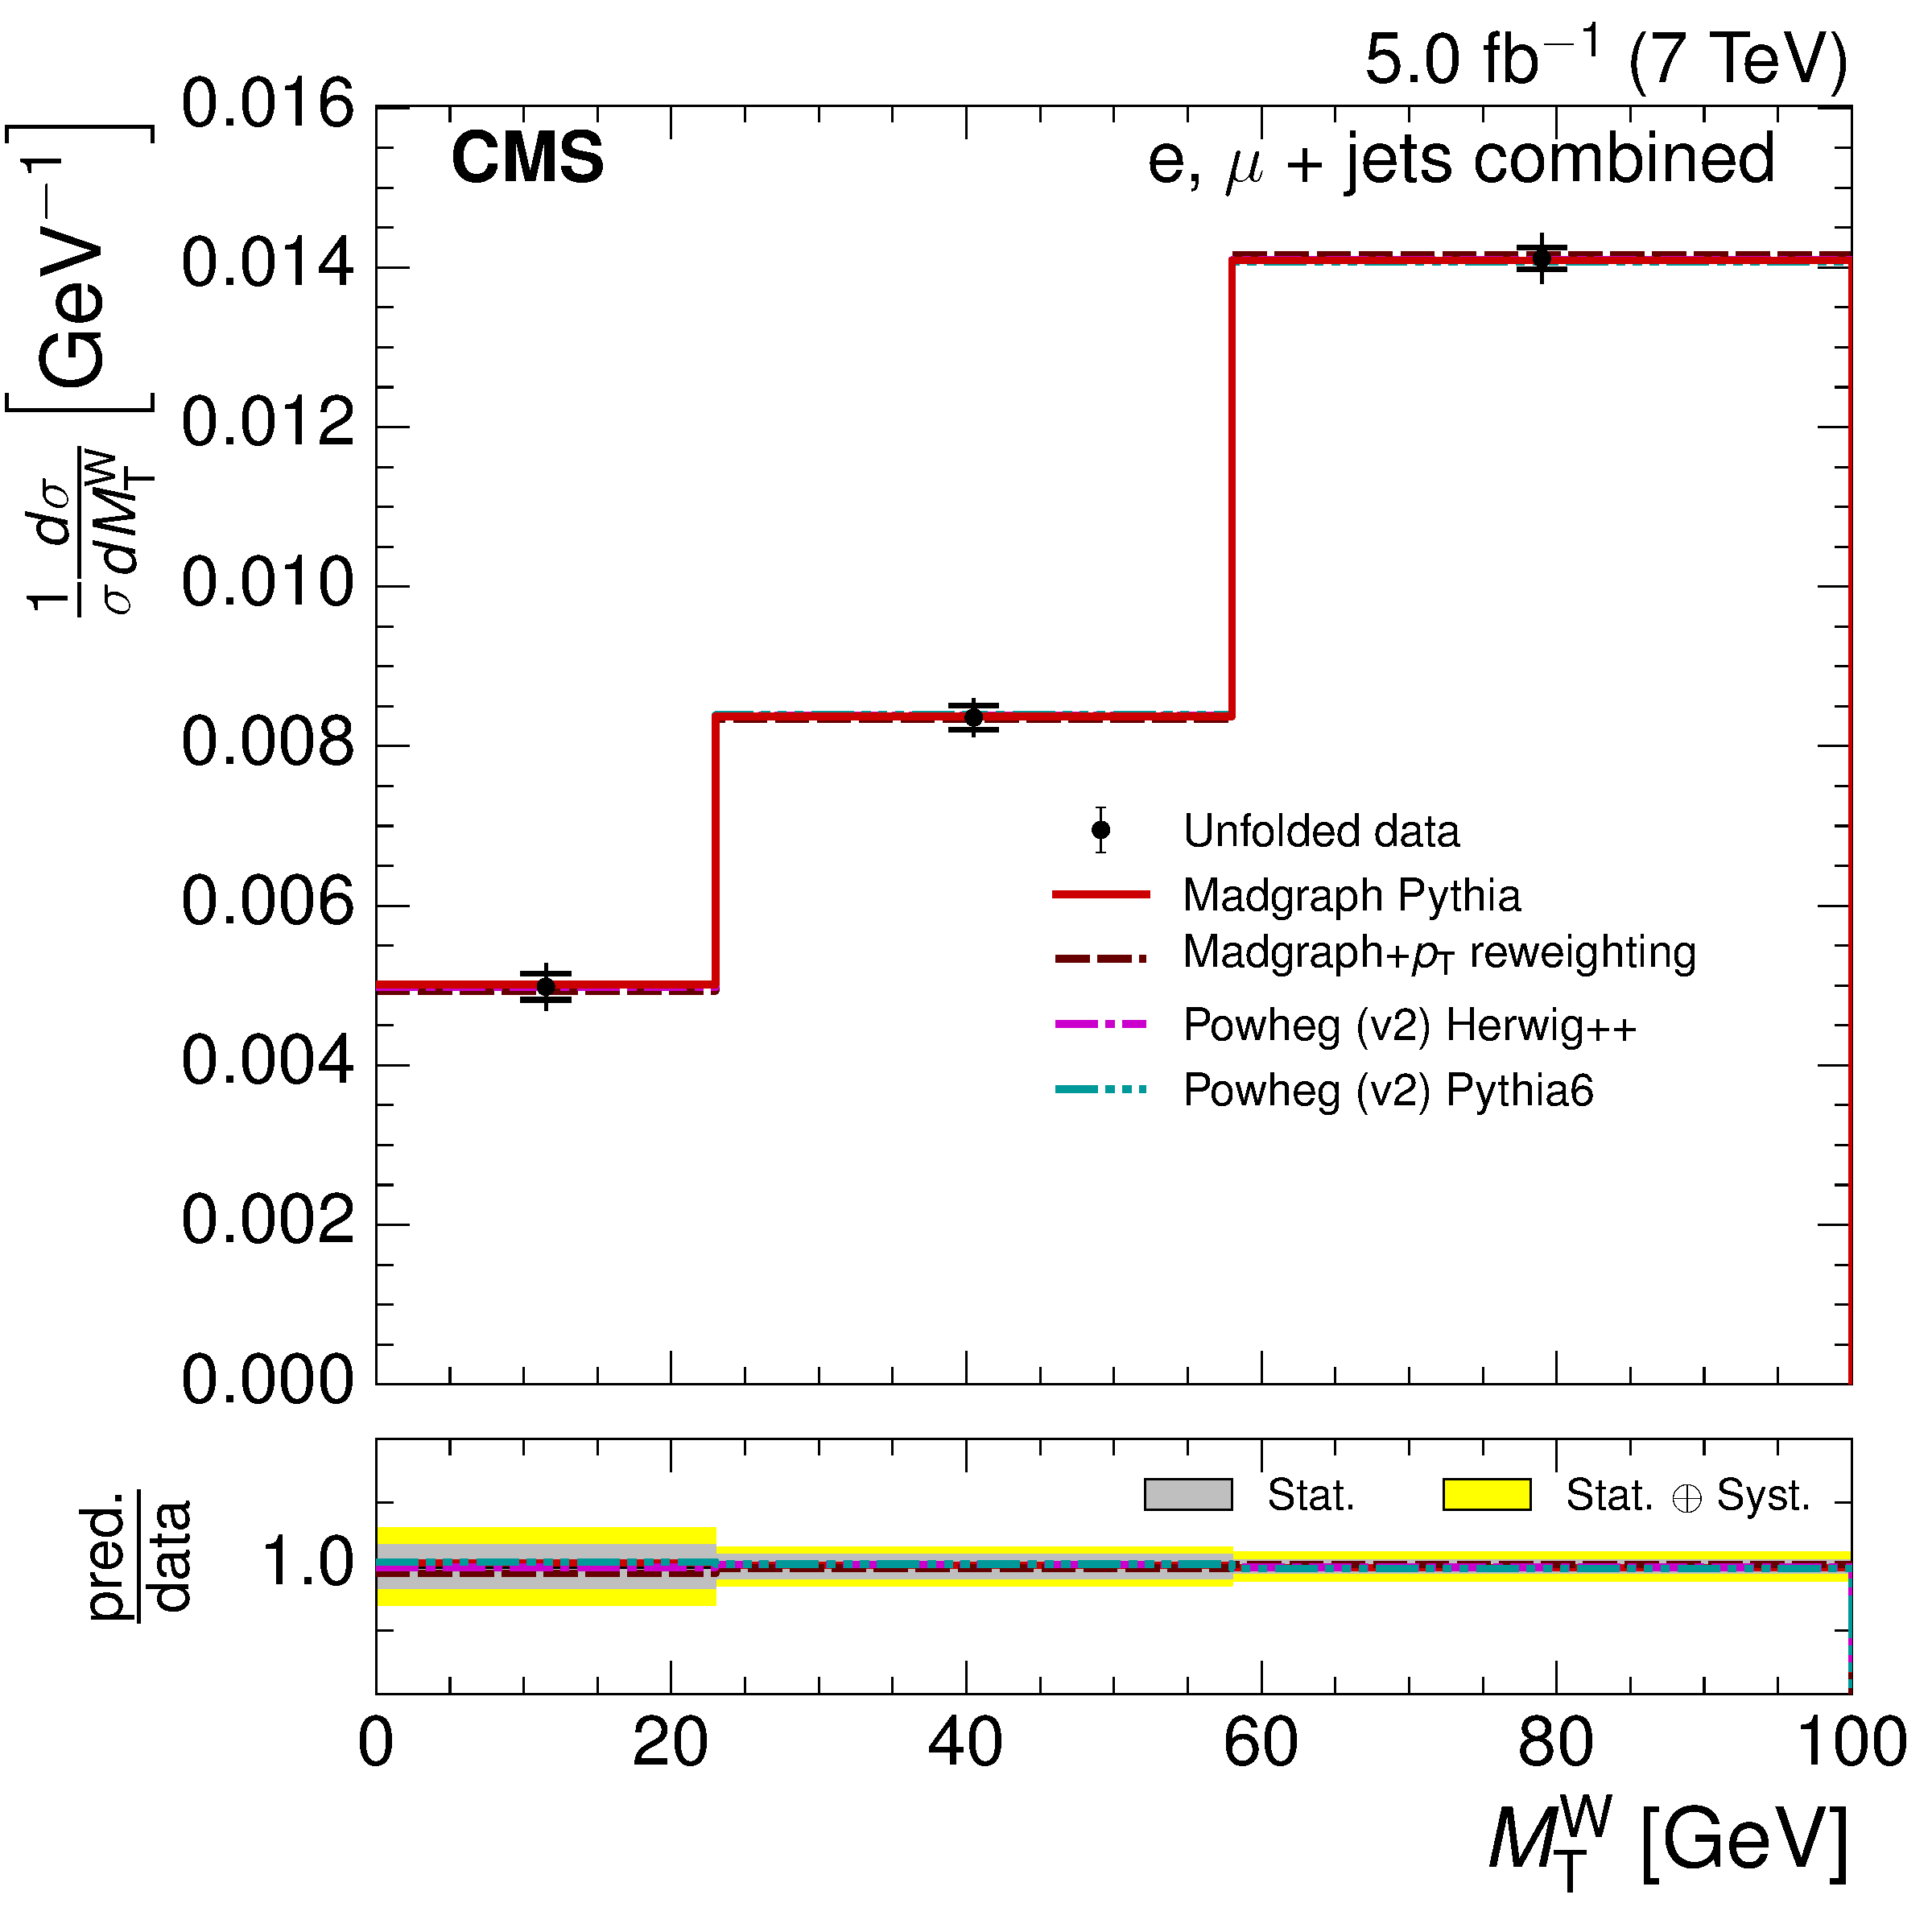
\includegraphics[width=0.48\textwidth]{Chapters/07_08_09_Analysis/Images/results/fit/7TeV/MT/central/normalised_xsection_combined_different_generators.pdf}\hfill
     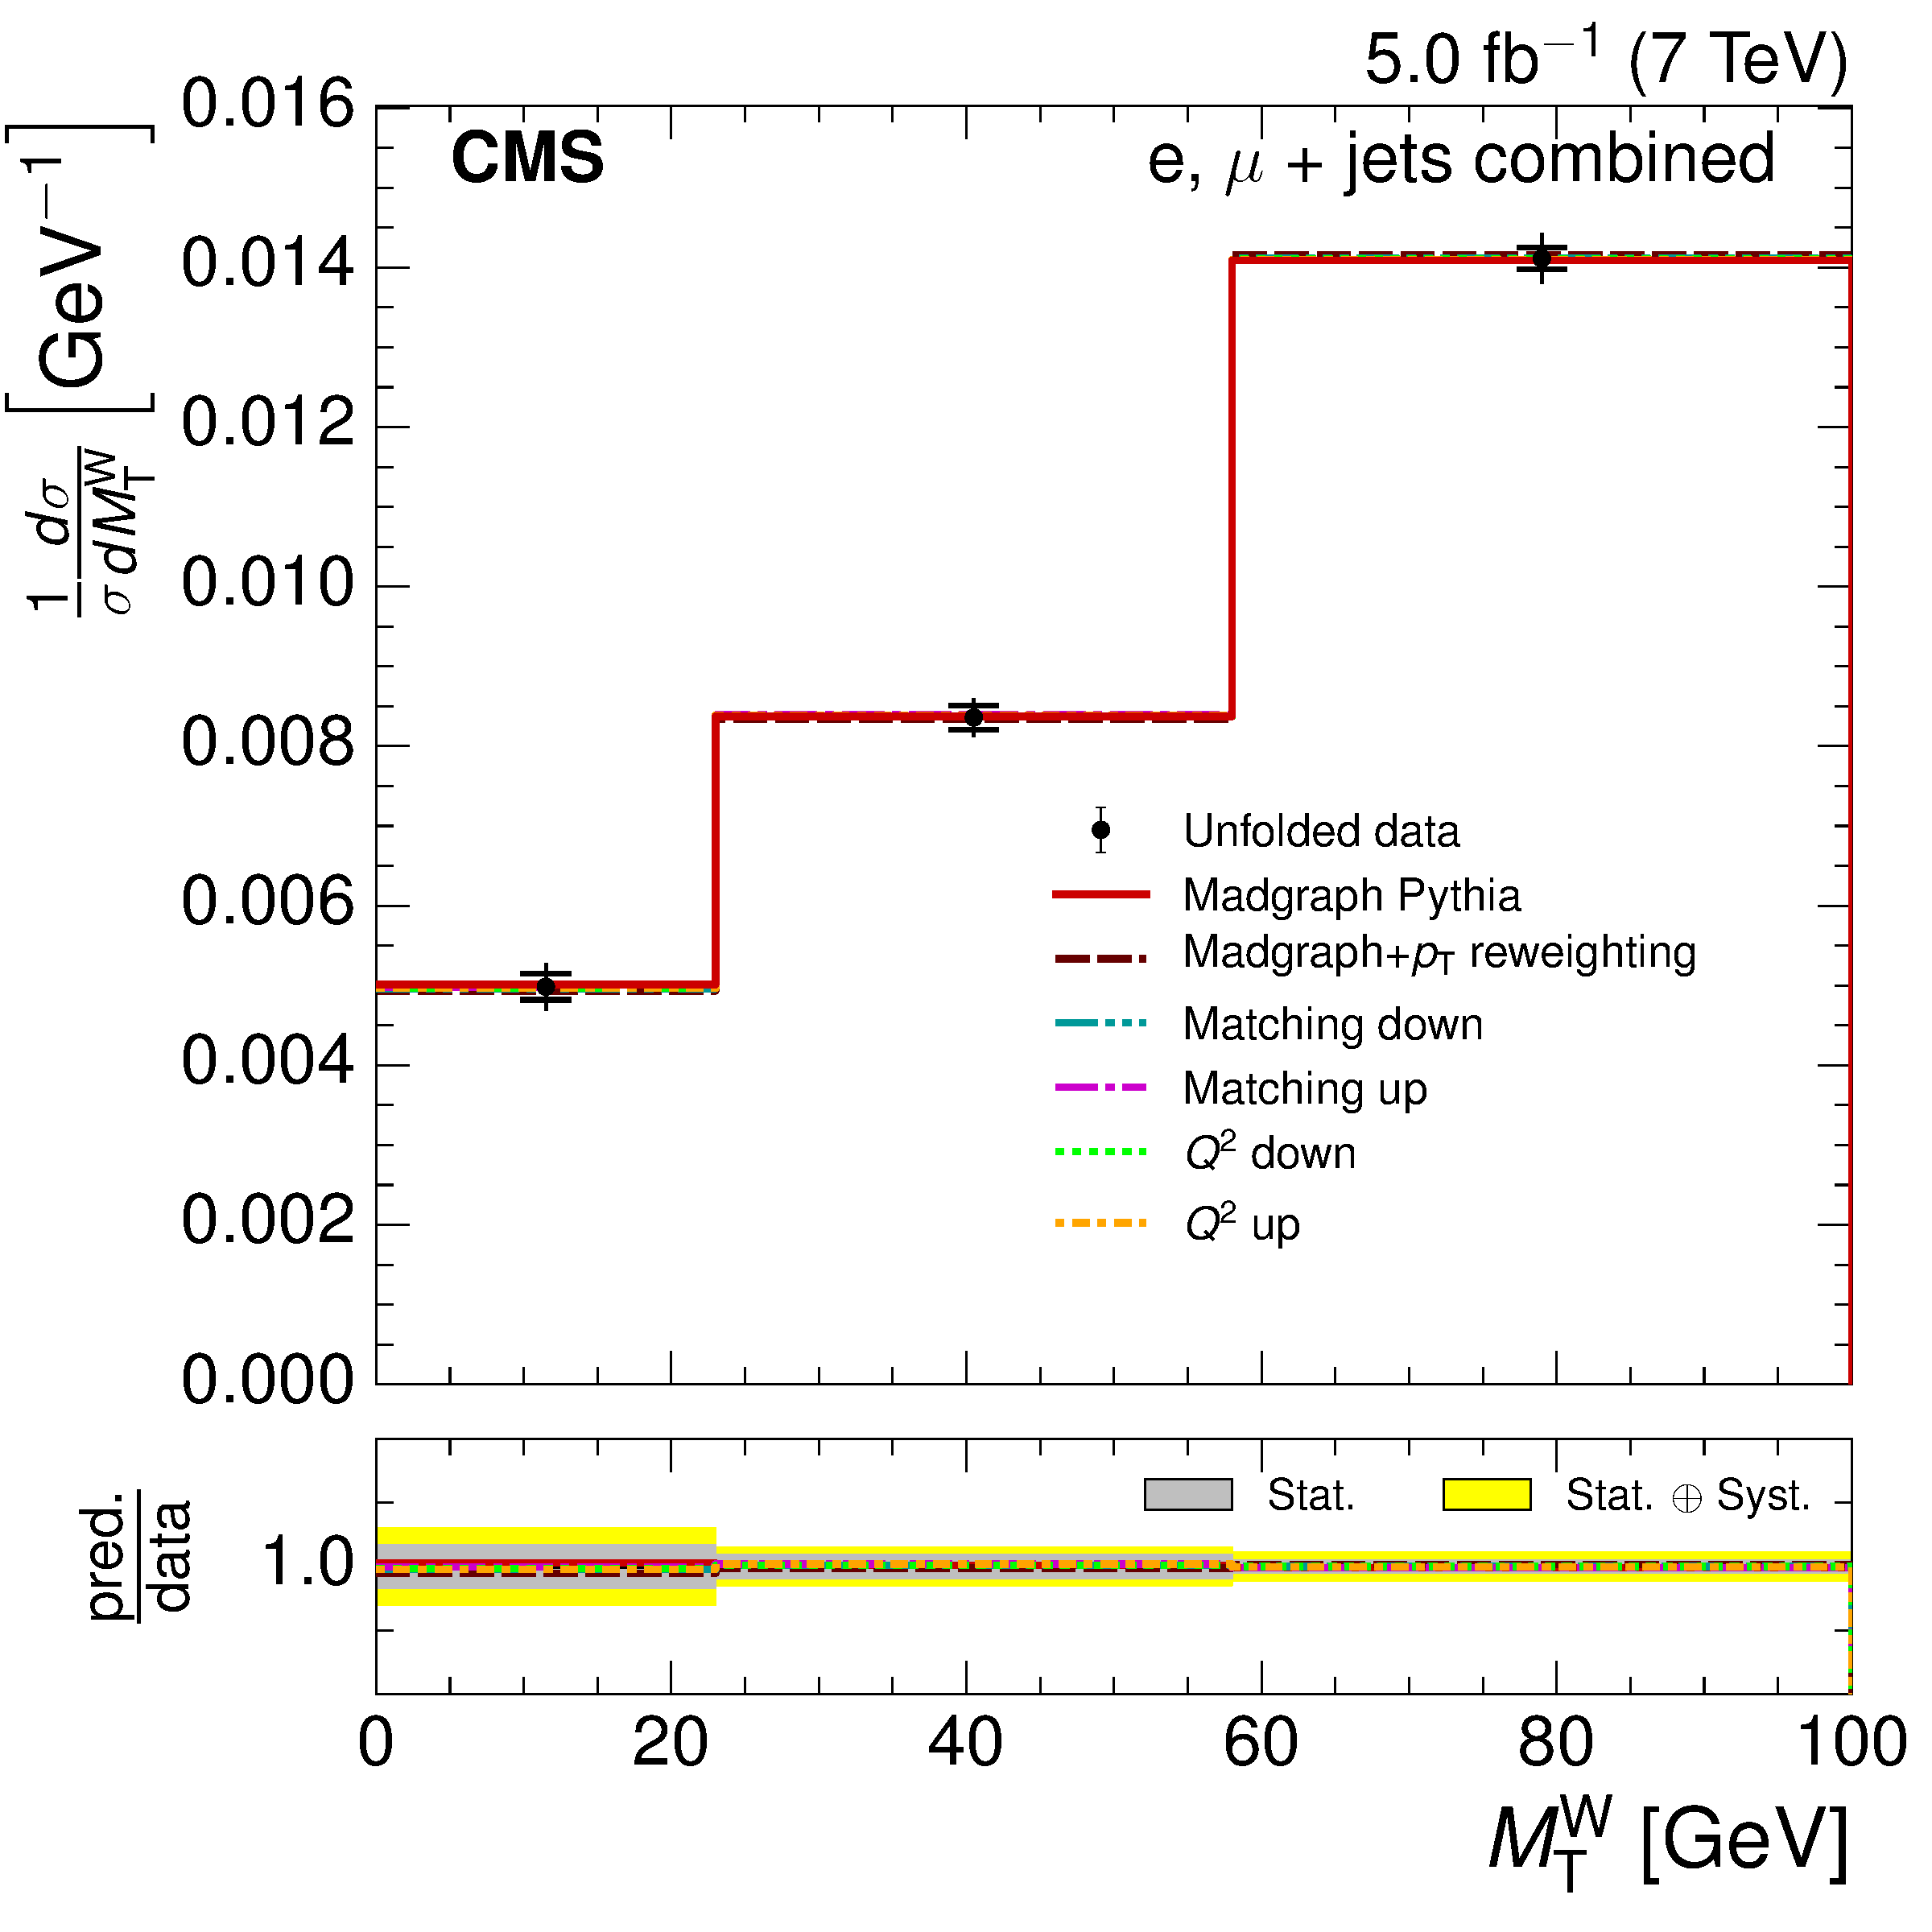
\includegraphics[width=0.48\textwidth]{Chapters/07_08_09_Analysis/Images/results/fit/7TeV/MT/central/normalised_xsection_combined_systematics_shifts.pdf}\hfill
     \caption[Comparison of the measured normalised differential cross section with respect to \wpt and \mt to
     different Monte Carlo generators and predictions at $\roots=7\TeV$.]{Comparison of the measured
     normalised differential cross section with respect to \wpt (upper) and \mt (lower) to different Monte
     Carlo generators:
     \MADGRAPH, \POWHEGHERWIG2, \POWHEGPYTHIA2 and \MADGRAPH corrected for top \pt mismodelling (left) and
     to different Monte Carlo predictions matching threshold up/down and factorisation scale up/down (right)
     in the combined electron+jets and muon+jets channel at $\roots=7\TeV$. The lower plots show the ratio of
     the predictions to the data.}
     \label{fig:result_WPT_MT_7TeV_combined}
\end{figure}


\begin{figure}[hbtp]
    \centering
     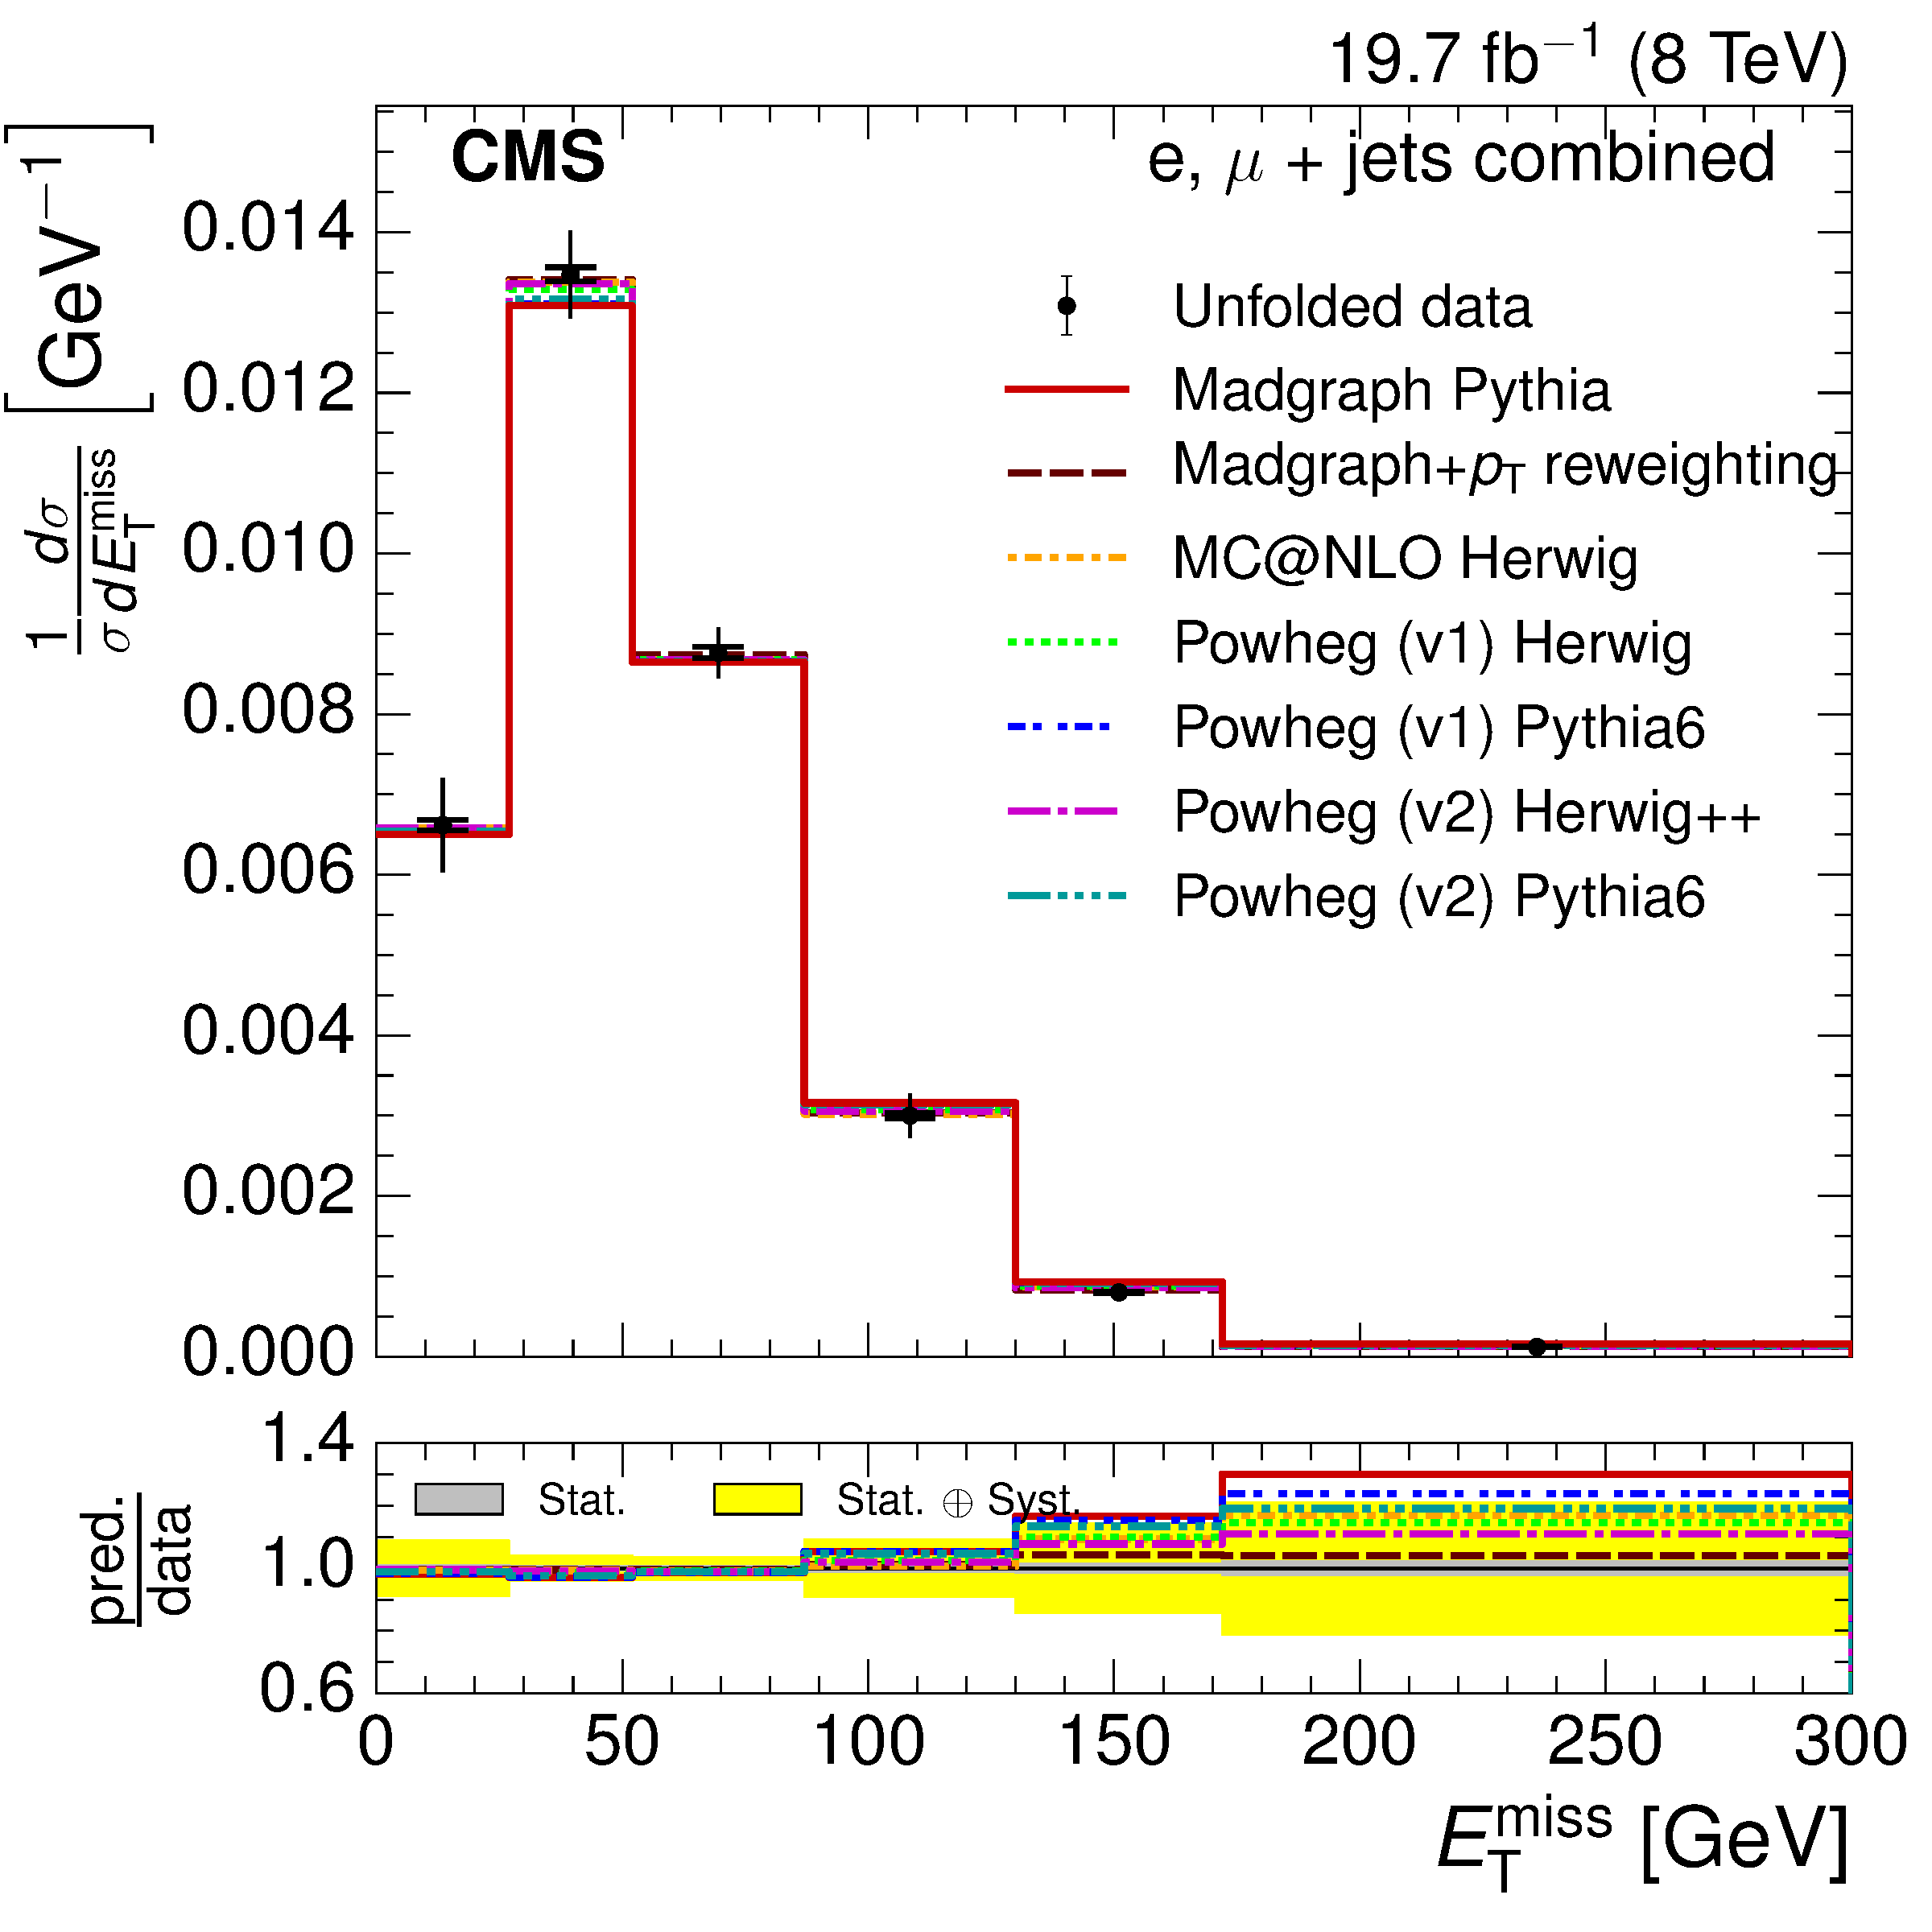
\includegraphics[width=0.435\textwidth]{Chapters/07_08_09_Analysis/Images/results/fit/8TeV/MET/central/normalised_xsection_combined_different_generators.pdf}\hfill
     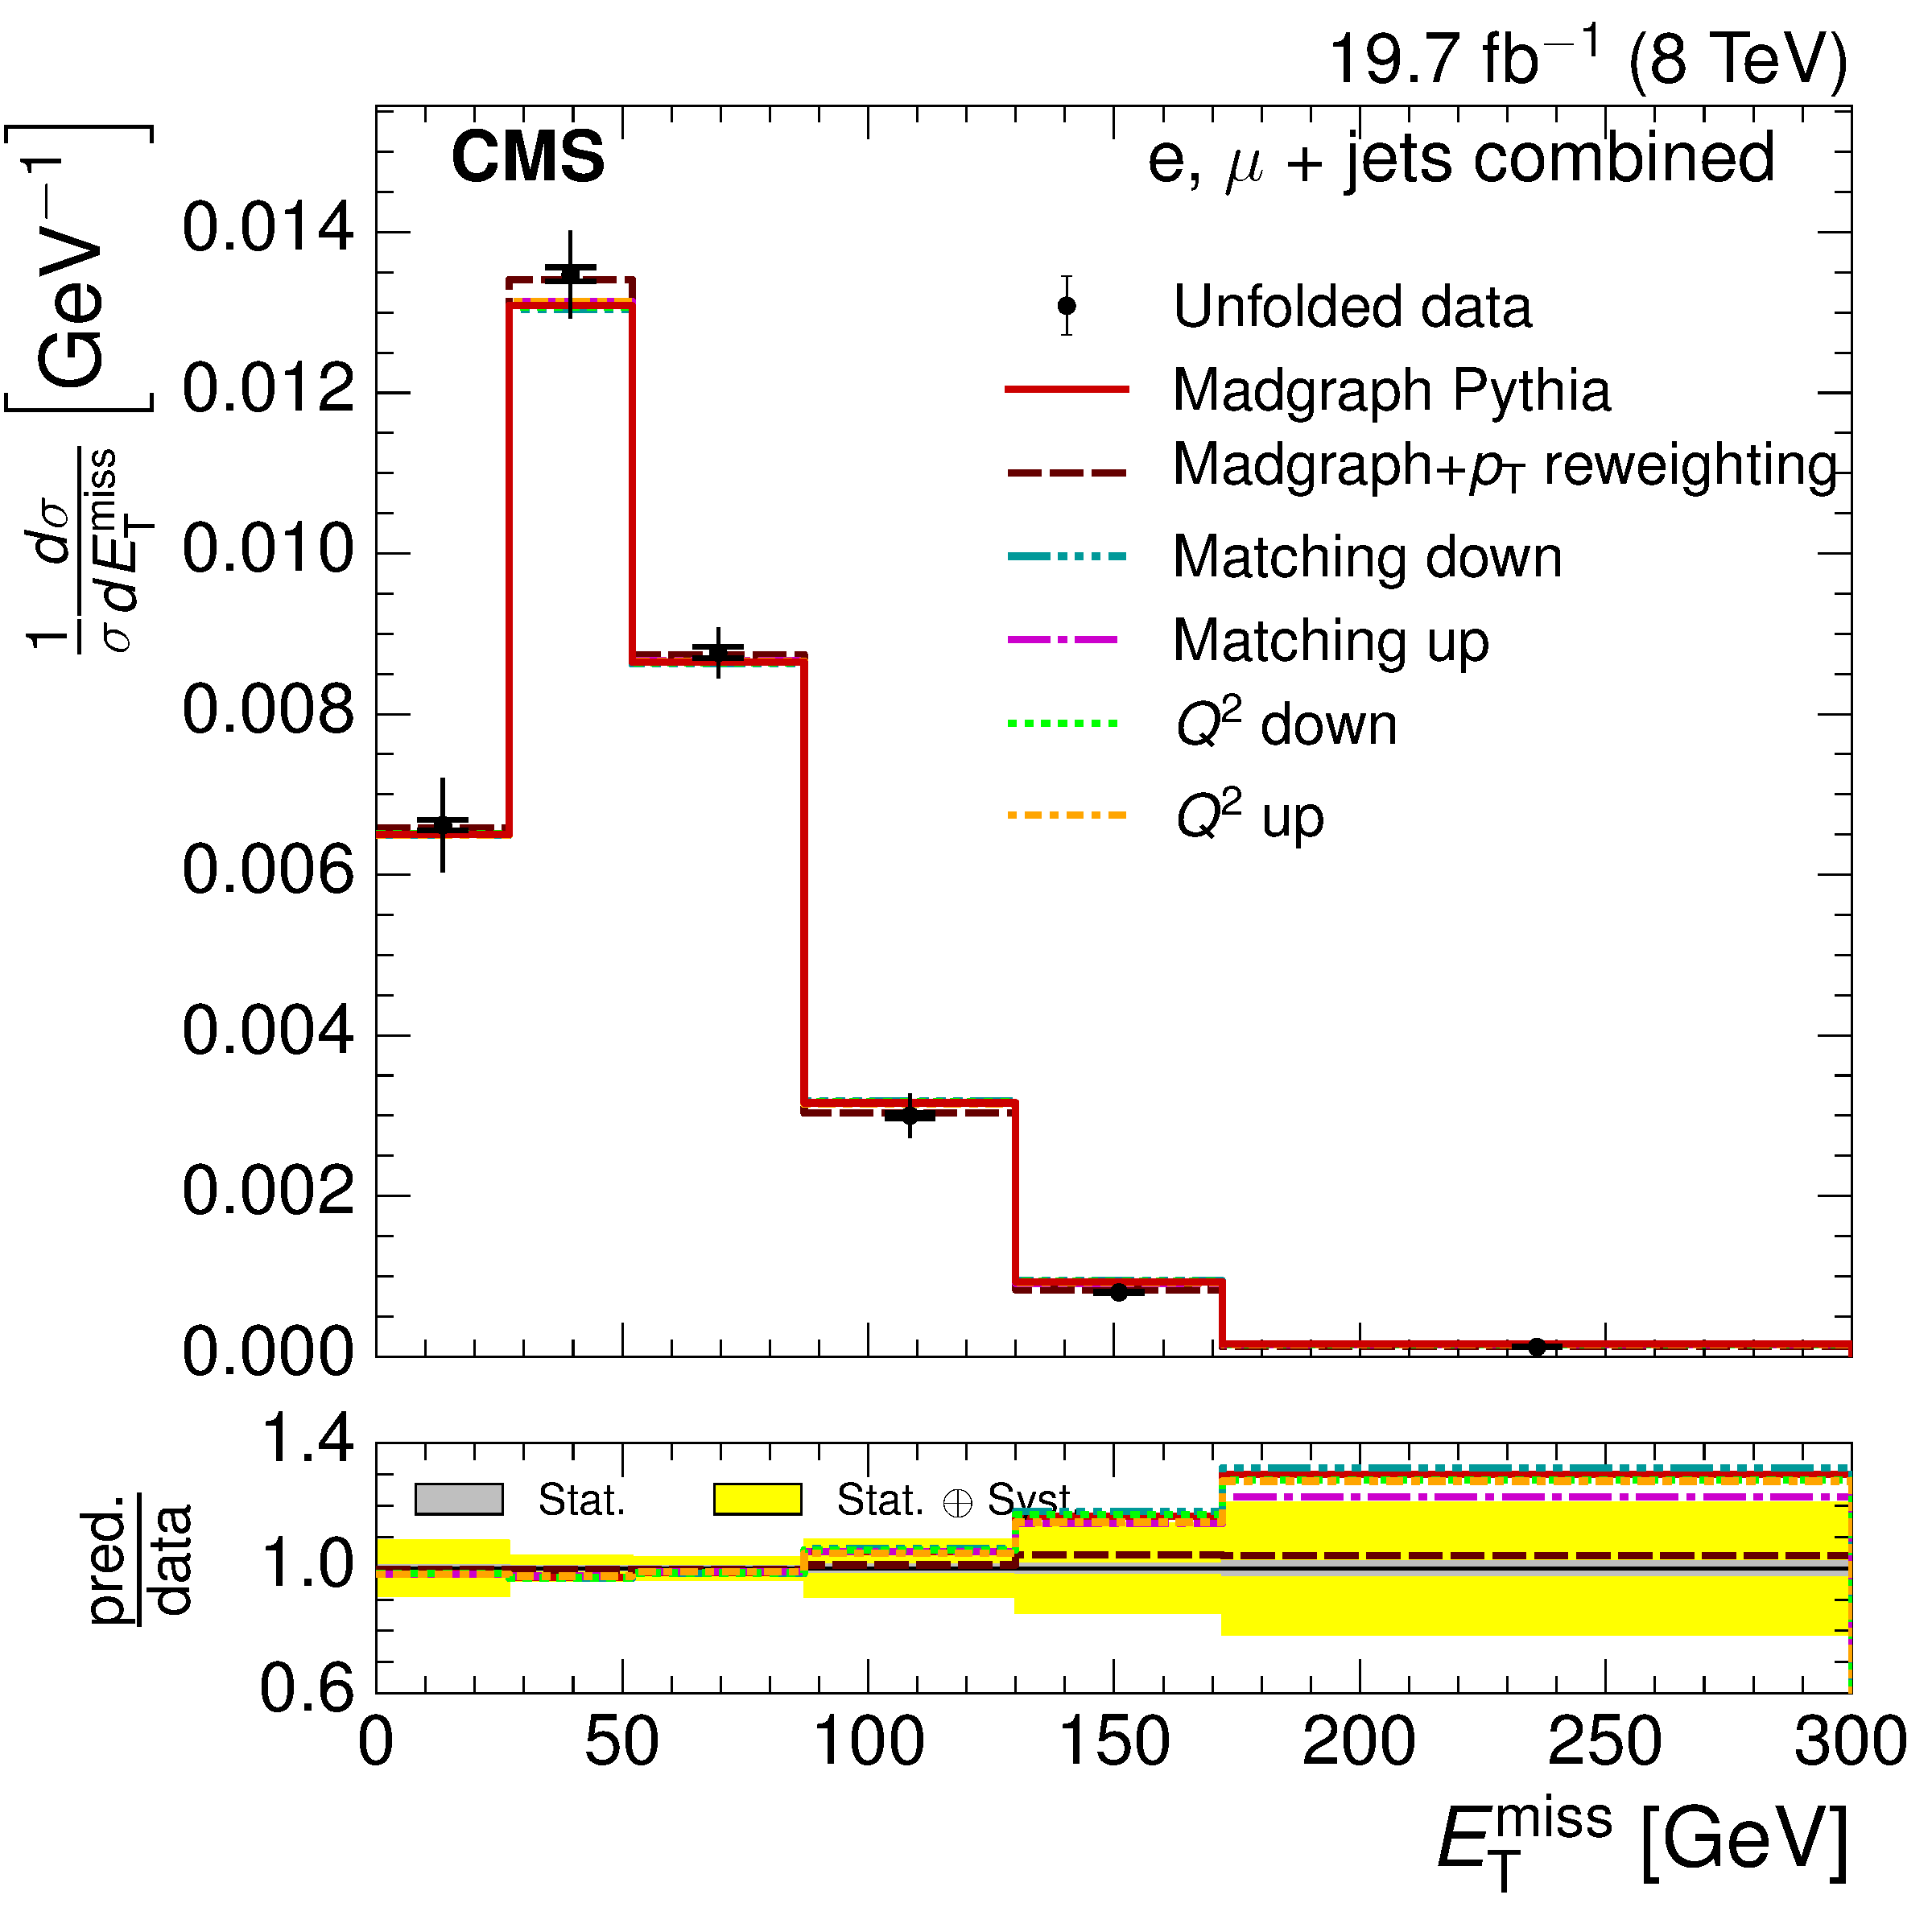
\includegraphics[width=0.435\textwidth]{Chapters/07_08_09_Analysis/Images/results/fit/8TeV/MET/central/normalised_xsection_combined_systematics_shifts.pdf}\hfill
     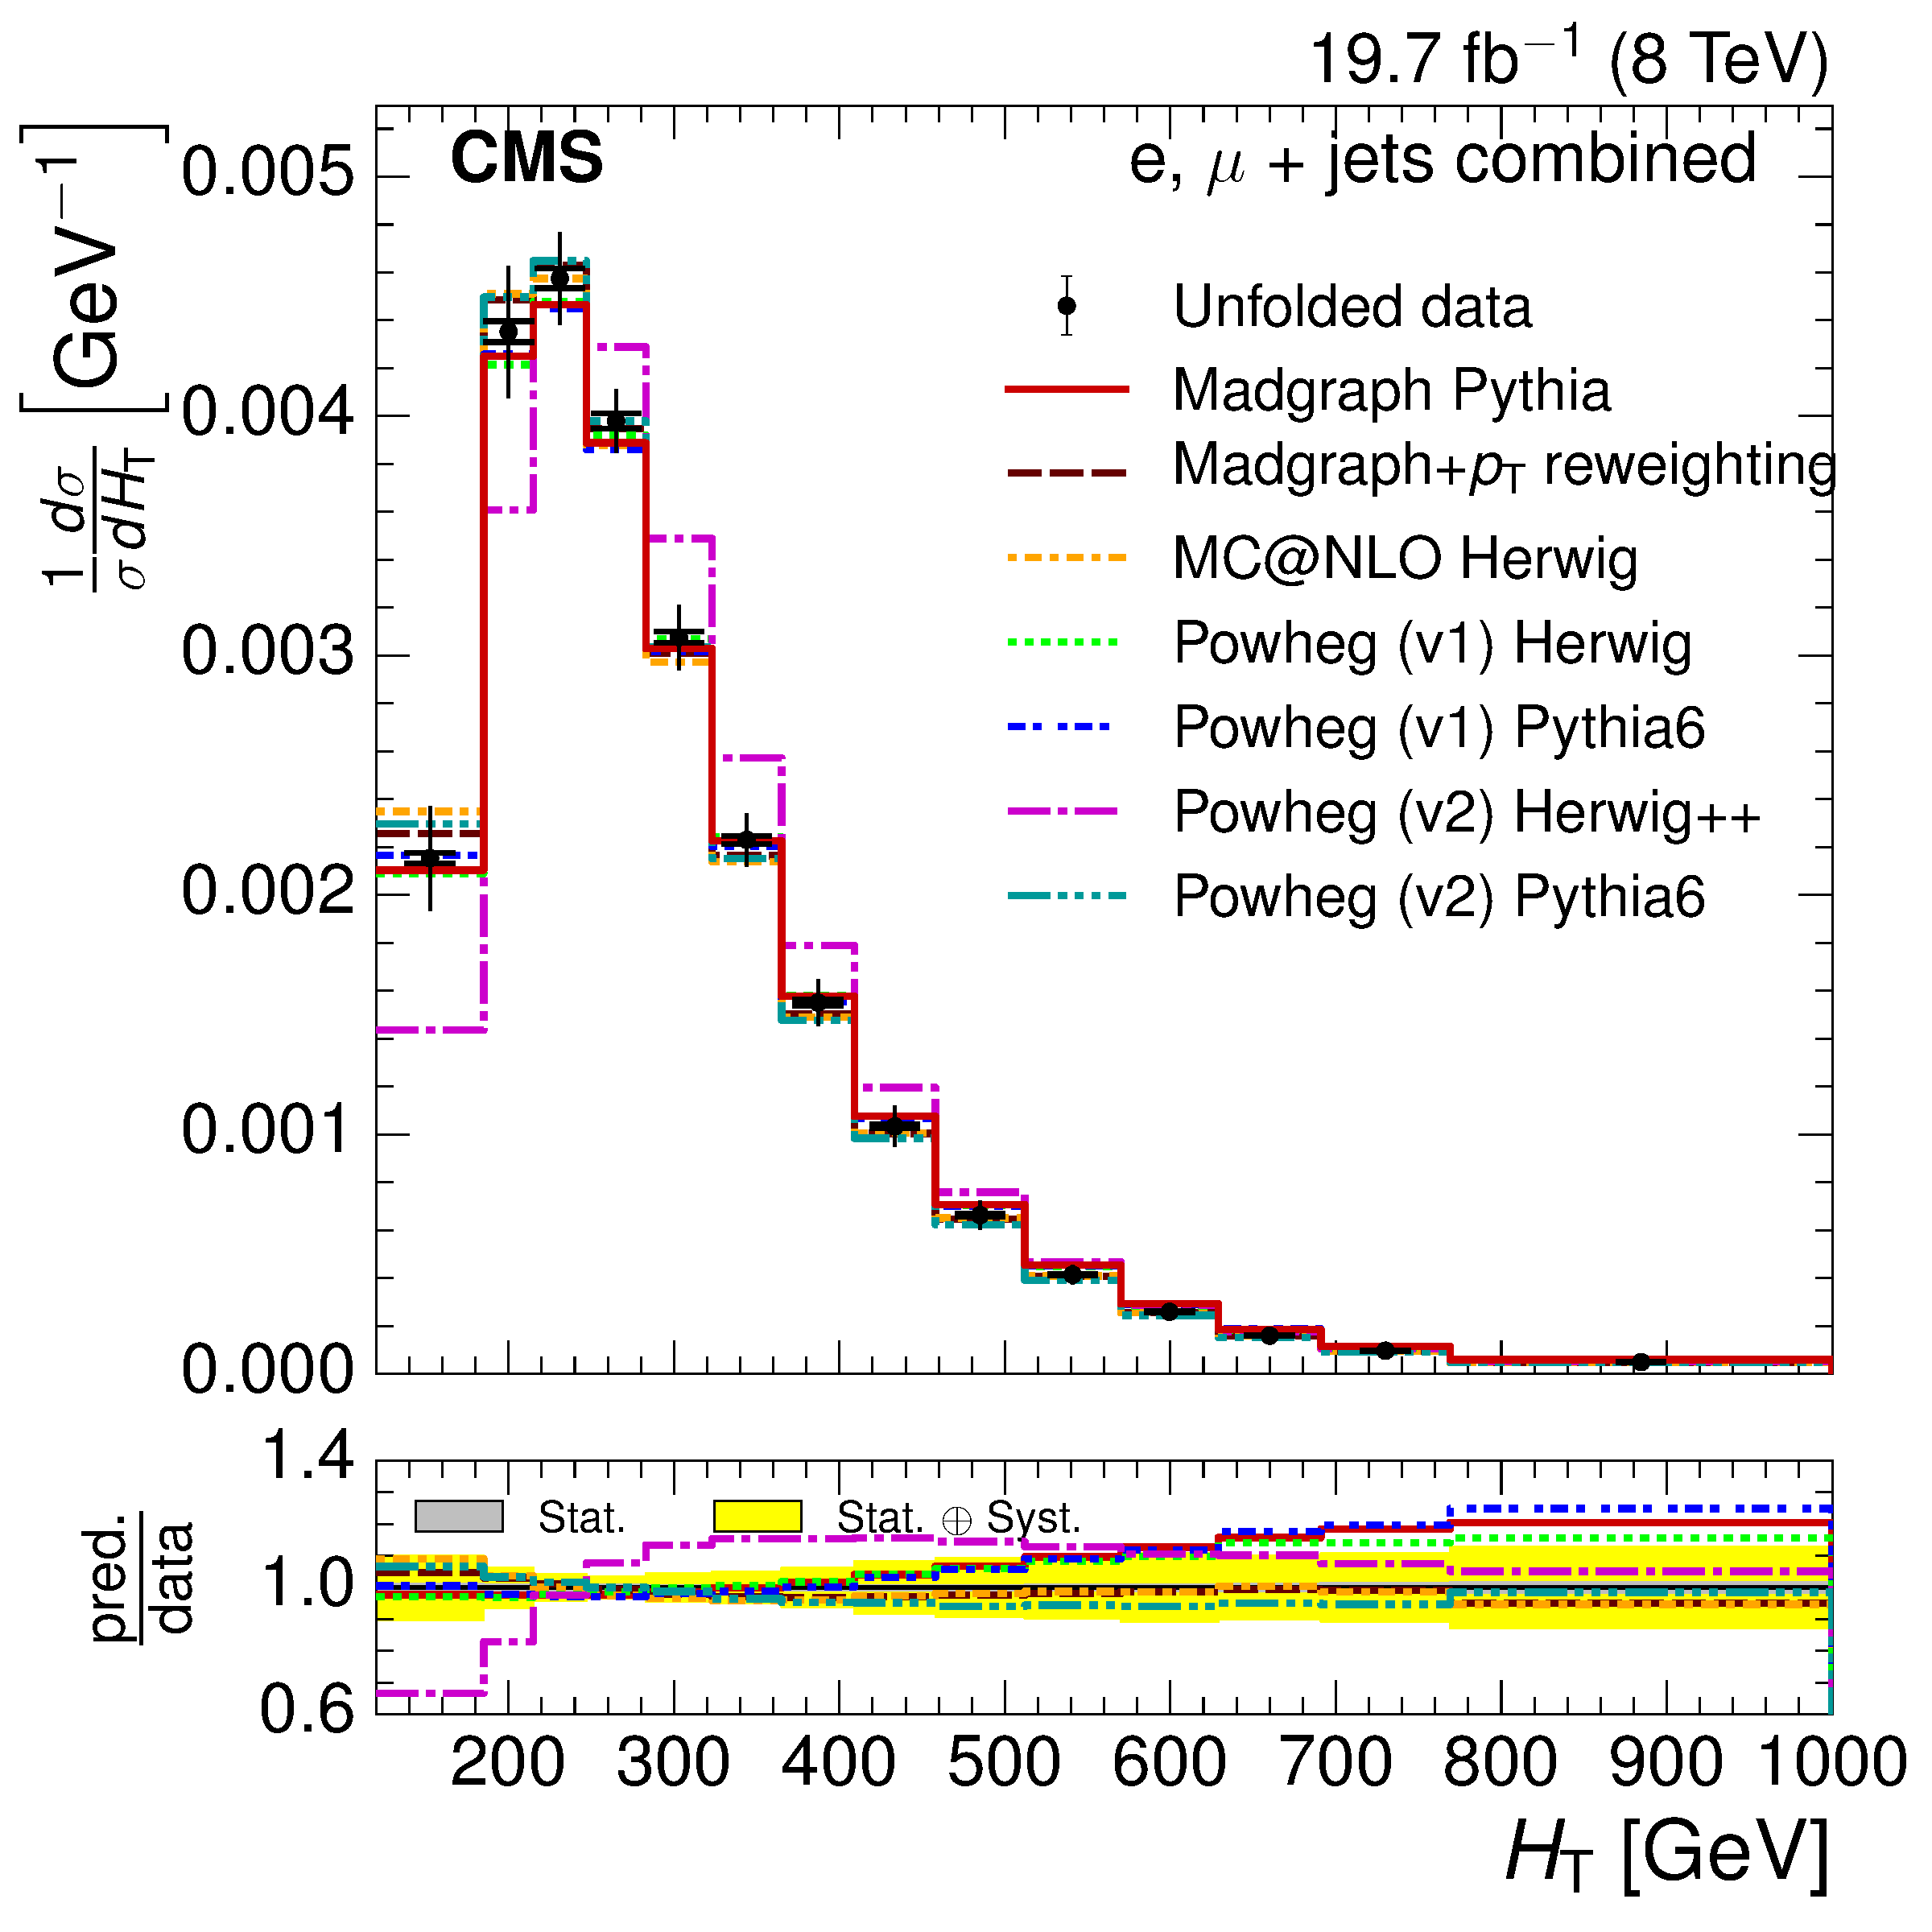
\includegraphics[width=0.435\textwidth]{Chapters/07_08_09_Analysis/Images/results/fit/8TeV/HT/central/normalised_xsection_combined_different_generators.pdf}\hfill
     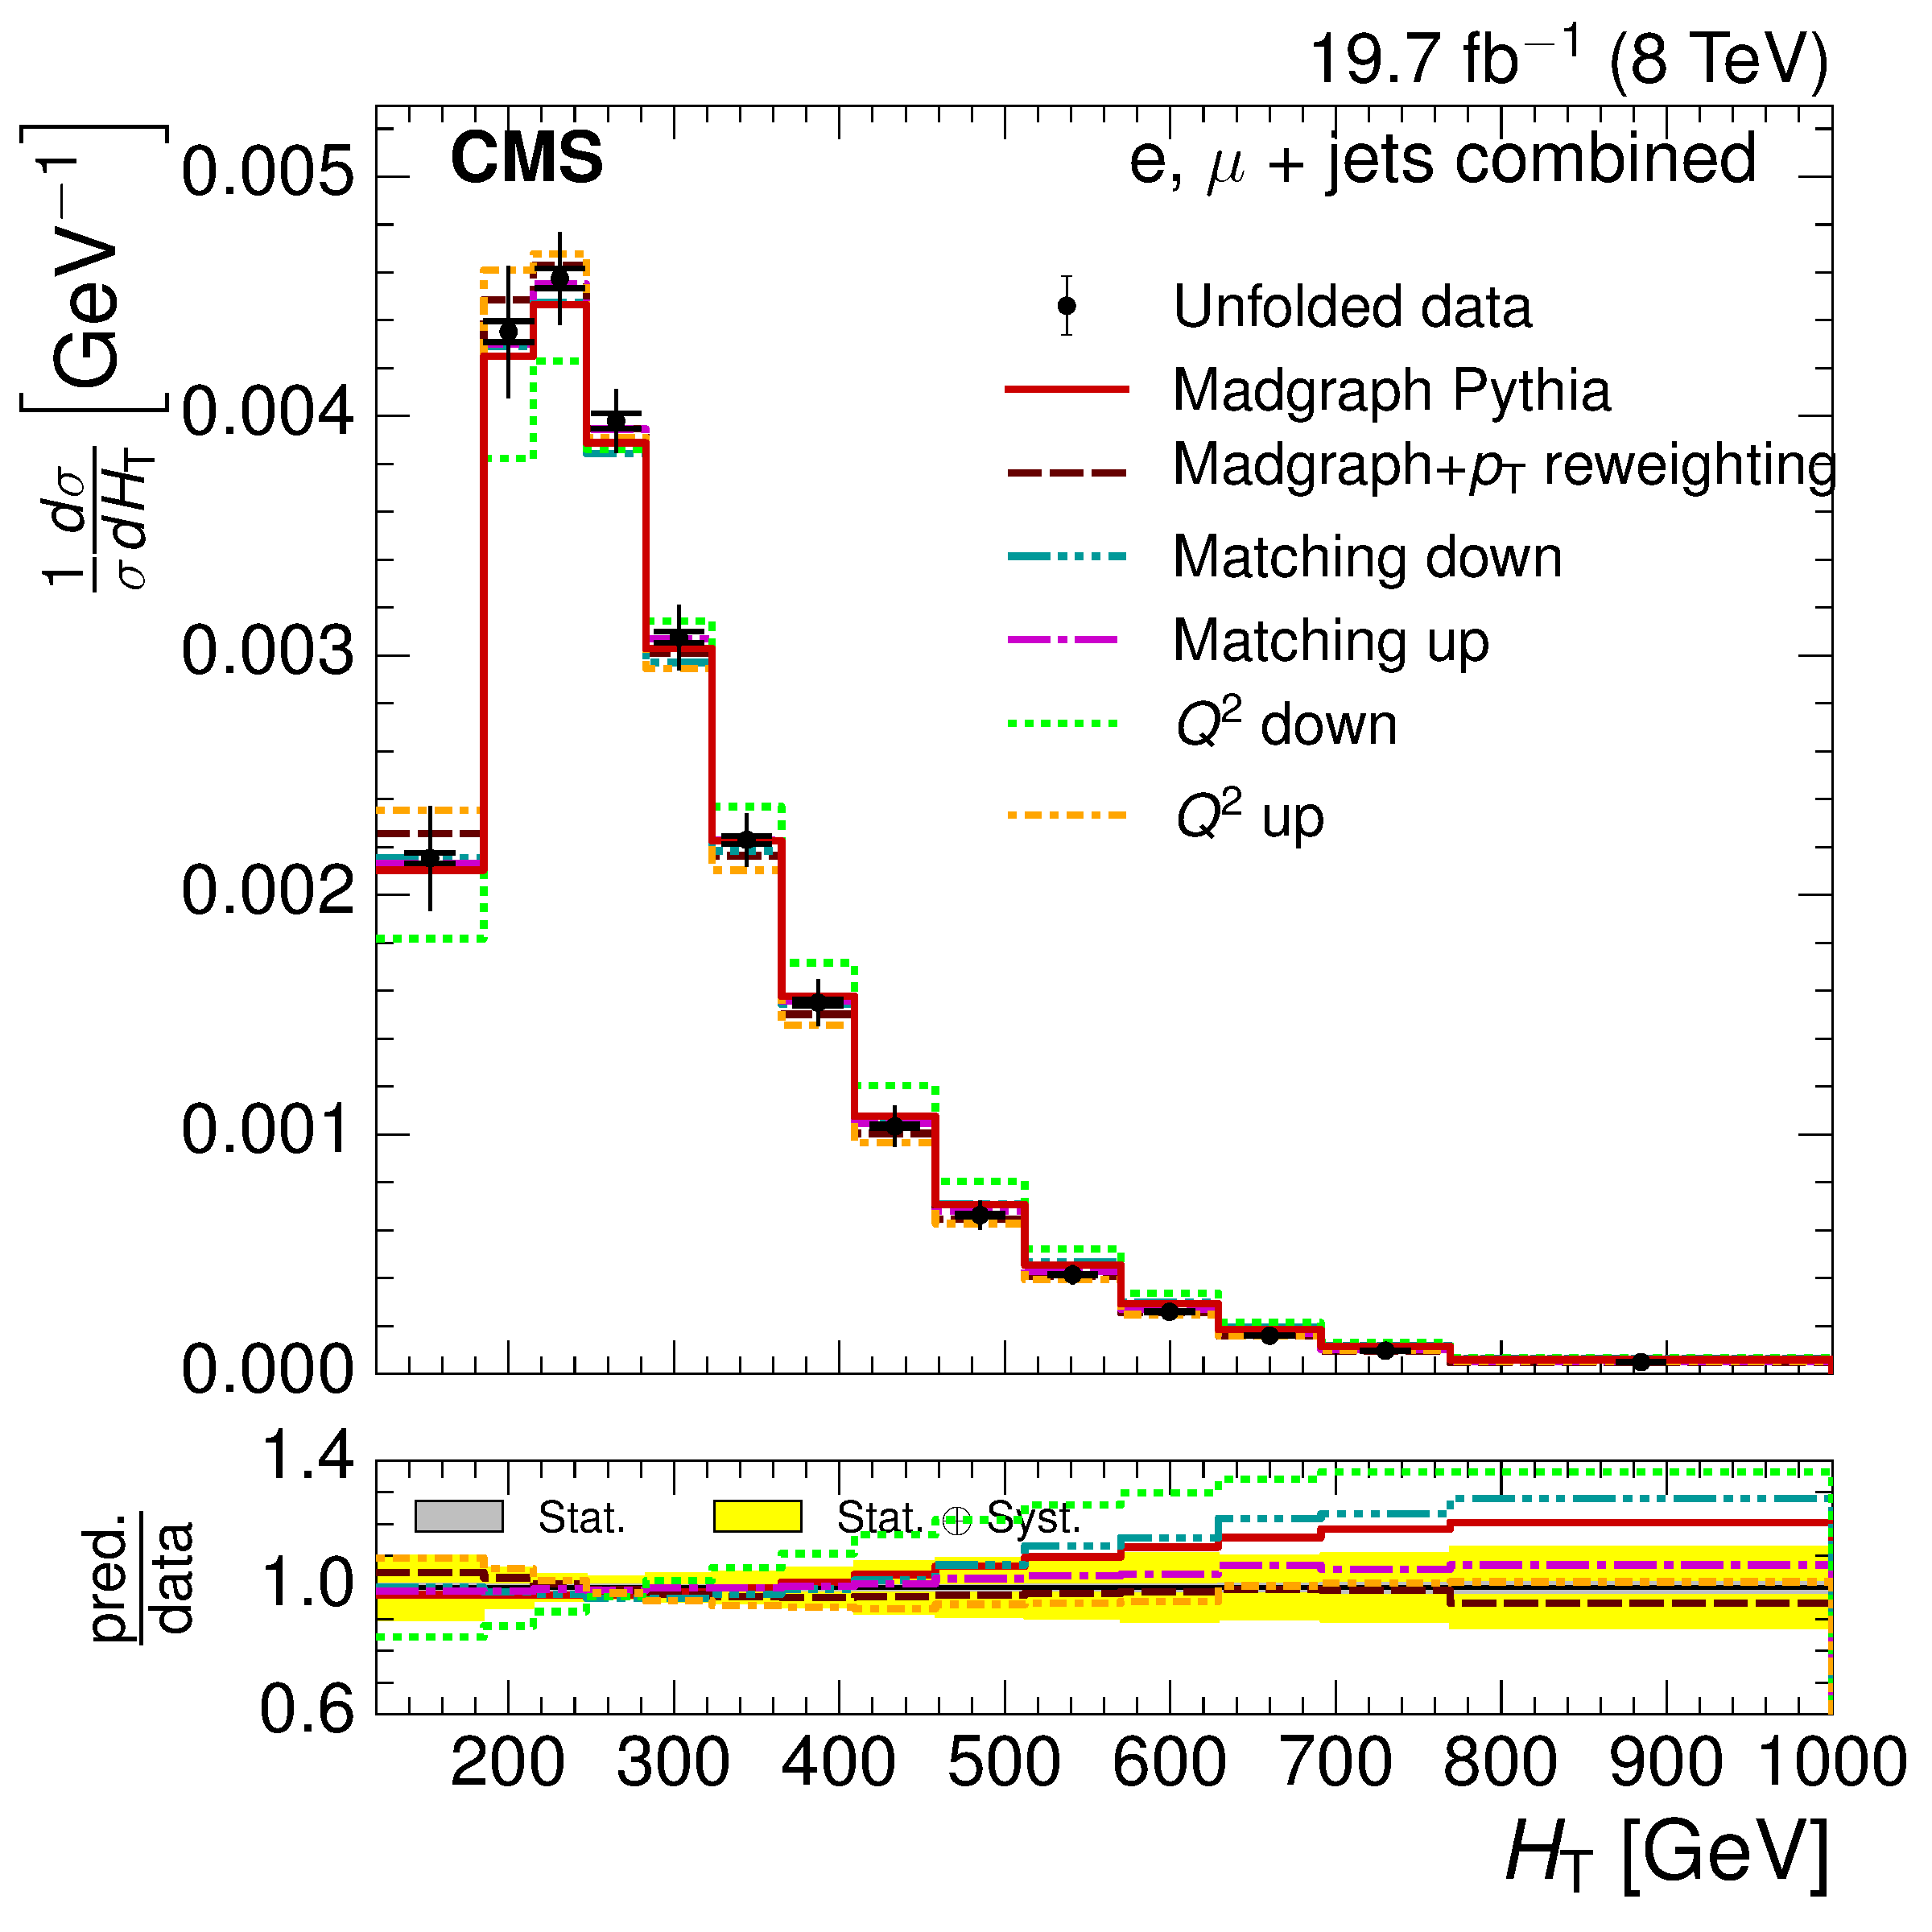
\includegraphics[width=0.435\textwidth]{Chapters/07_08_09_Analysis/Images/results/fit/8TeV/HT/central/normalised_xsection_combined_systematics_shifts.pdf}\hfill
     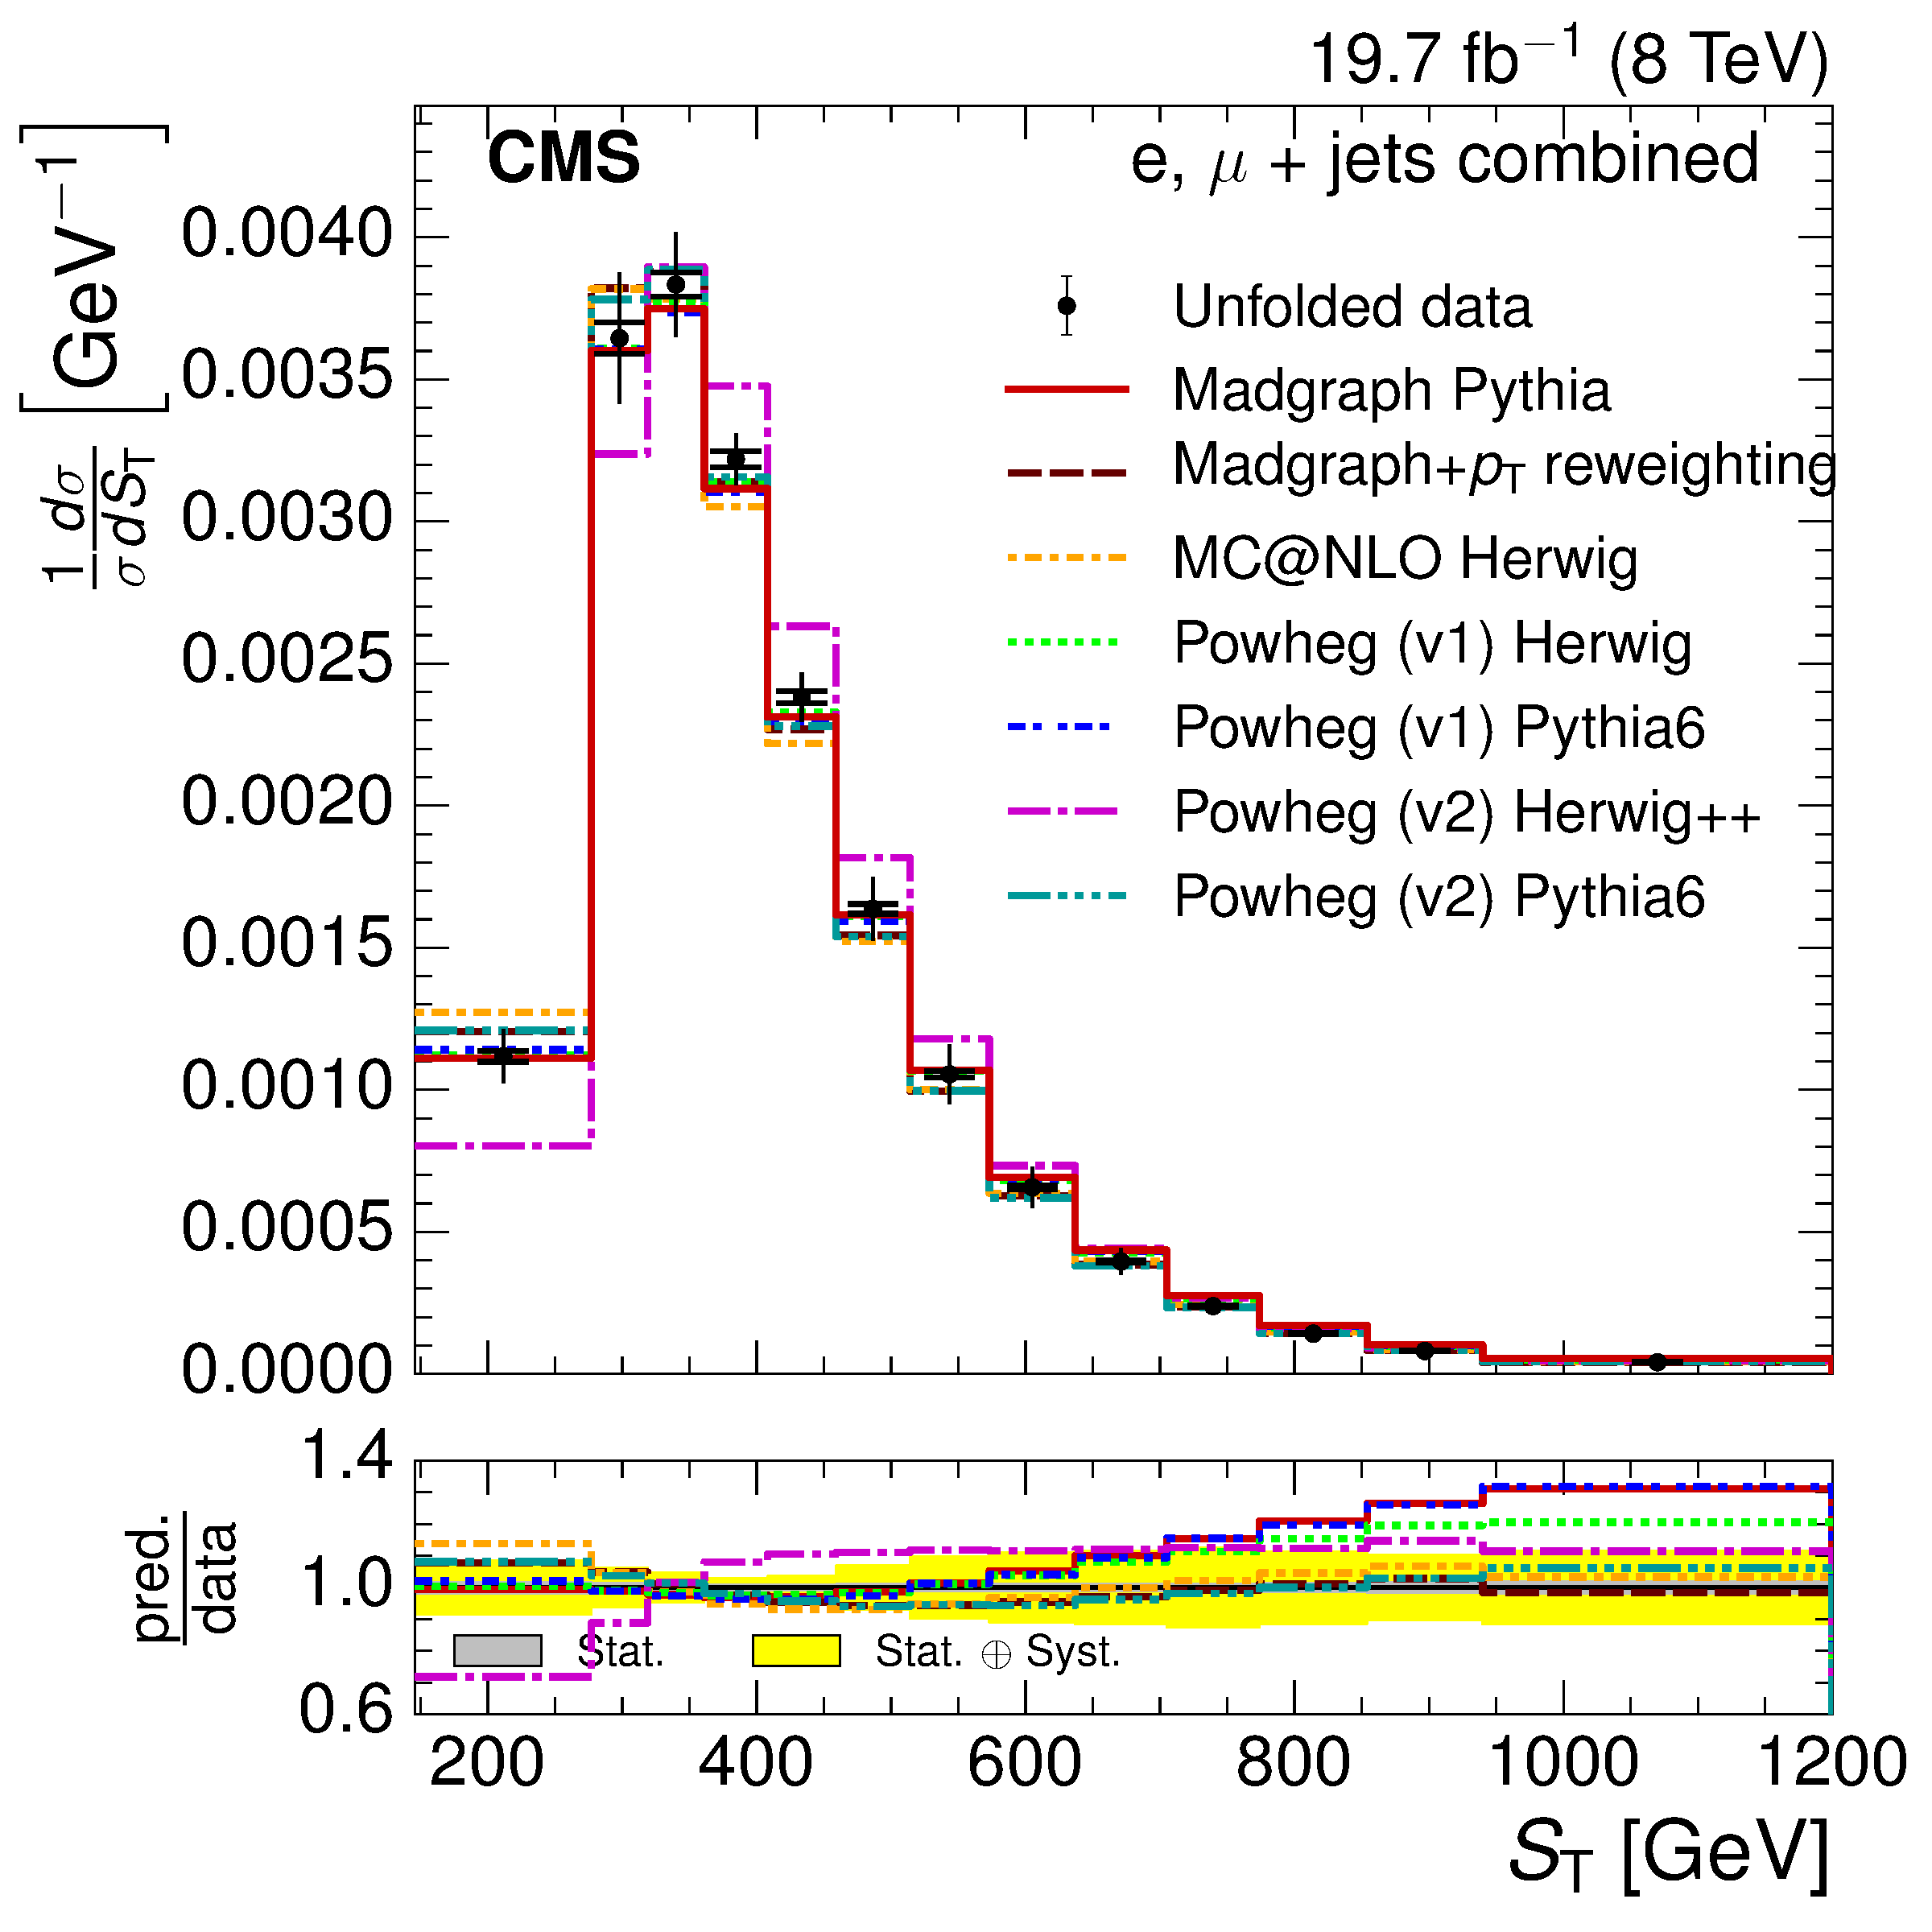
\includegraphics[width=0.435\textwidth]{Chapters/07_08_09_Analysis/Images/results/fit/8TeV/ST/central/normalised_xsection_combined_different_generators.pdf}\hfill
     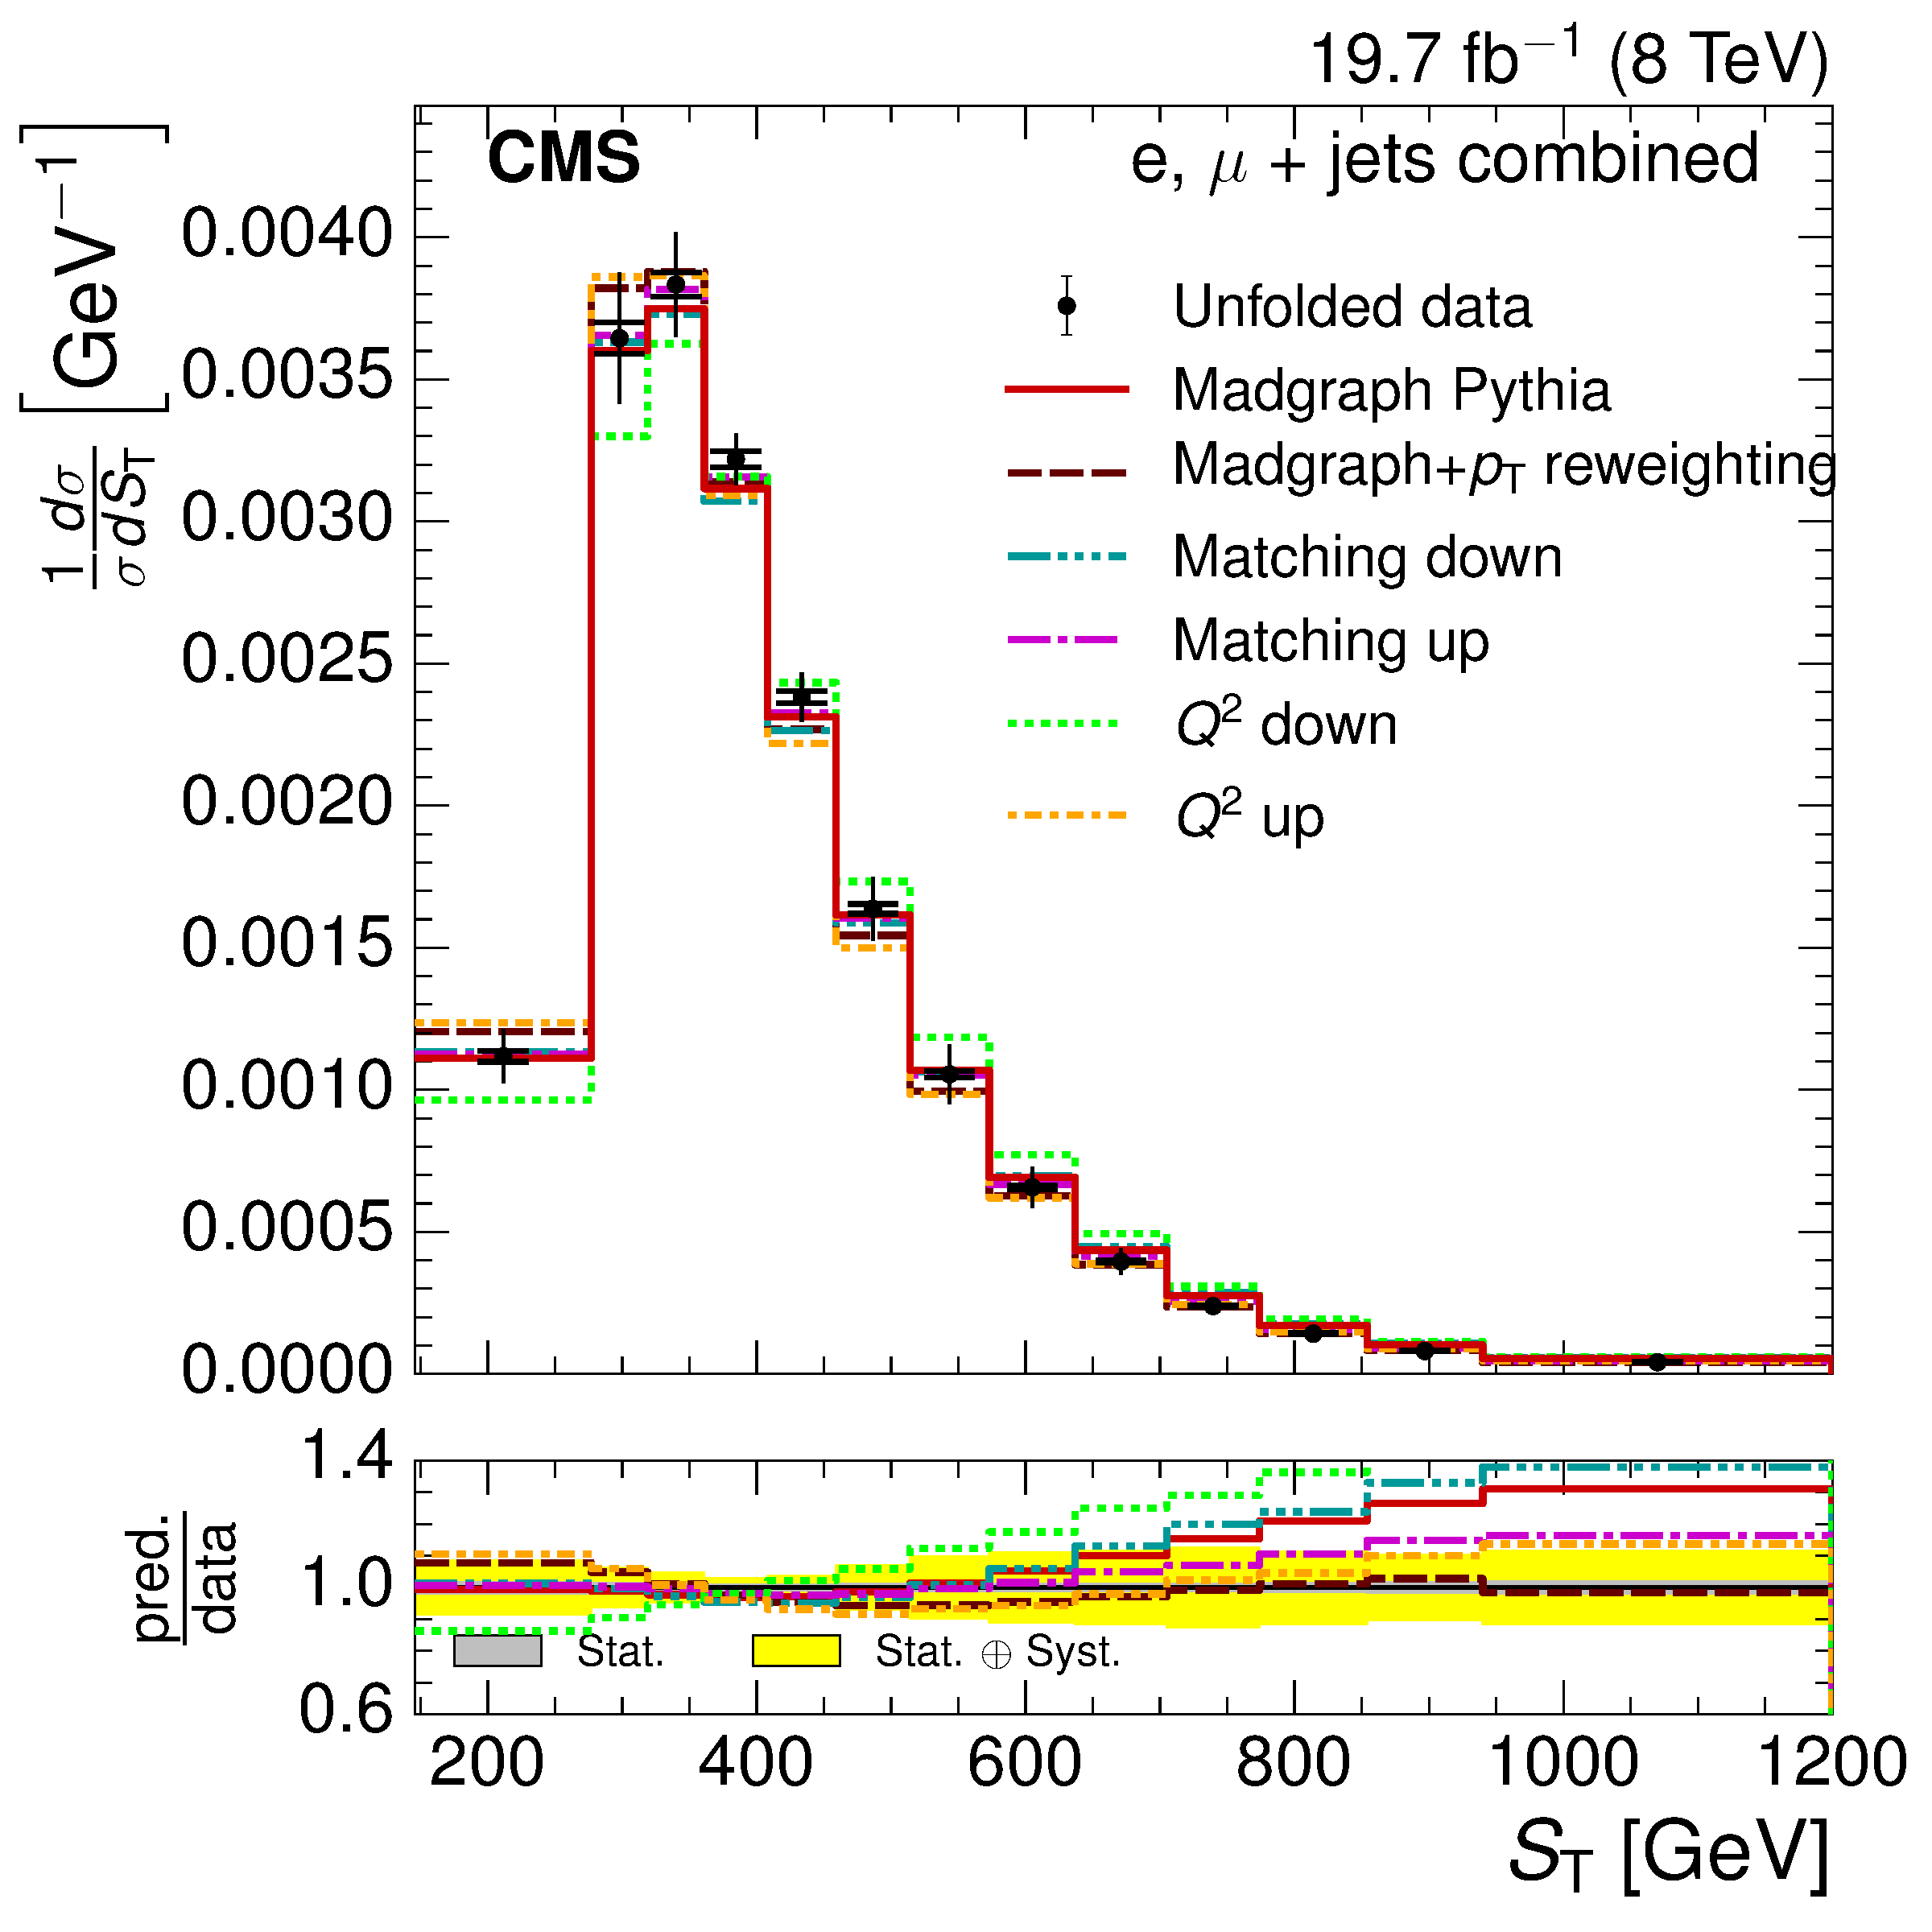
\includegraphics[width=0.435\textwidth]{Chapters/07_08_09_Analysis/Images/results/fit/8TeV/ST/central/normalised_xsection_combined_systematics_shifts.pdf}\hfill
     \caption[Comparison of the measured normalised differential cross section with respect to \met, \HT and
     \st to different Monte Carlo generators and predictions at $\roots=8\TeV$.]{Comparison of the measured
     normalised differential cross section with respect to \met (upper), \HT (middle) and \st (lower) to
     different Monte Carlo generators: \MADGRAPH, \POWHEGHERWIG1, \POWHEGPYTHIA1, \POWHEGHERWIG2,
     \POWHEGPYTHIA2 and \MADGRAPH corrected for top \pt mismodelling (left) and to different Monte Carlo
     predictions matching threshold up/down and factorisation scale up/down (right) in the combined
     electron+jets and muon+jets channel at $\roots=8\TeV$. The lower plots show the ratio of the predictions
     to the data.}
     \label{fig:result_MET_HT_ST_8TeV_combined}
\end{figure}

\begin{figure}[hbtp]
    \centering
     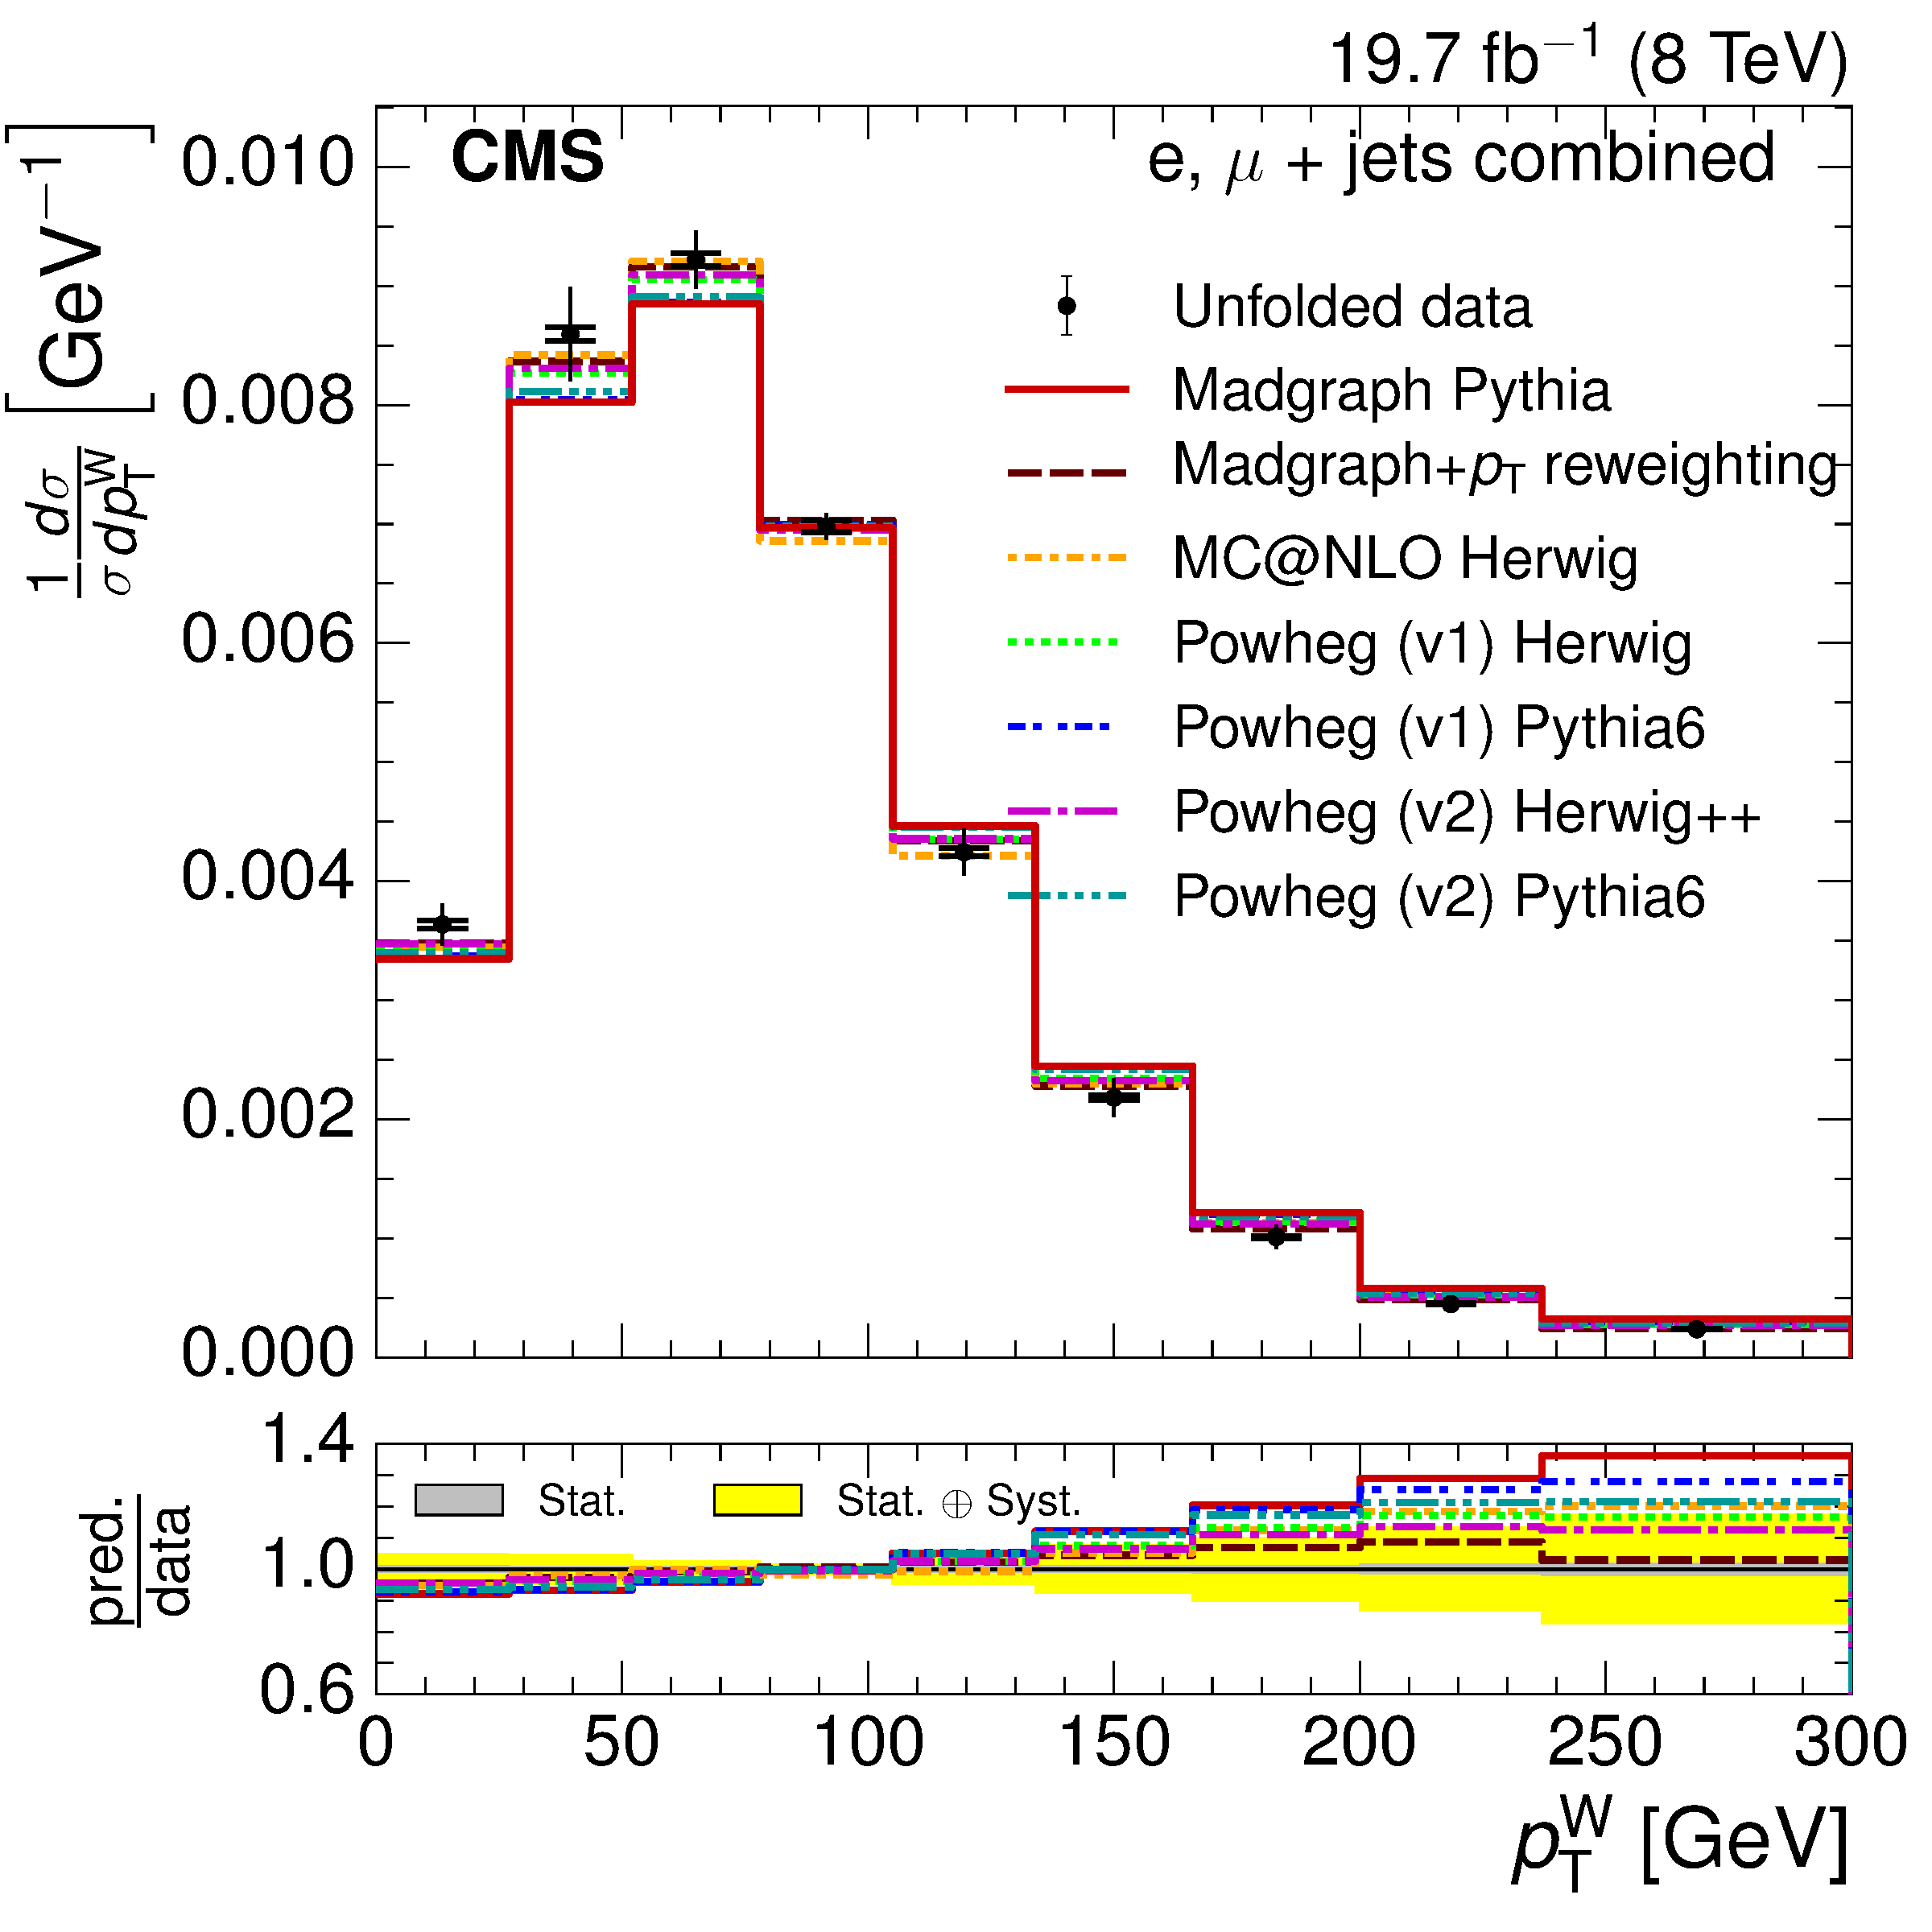
\includegraphics[width=0.48\textwidth]{Chapters/07_08_09_Analysis/Images/results/fit/8TeV/WPT/central/normalised_xsection_combined_different_generators.pdf}\hfill
     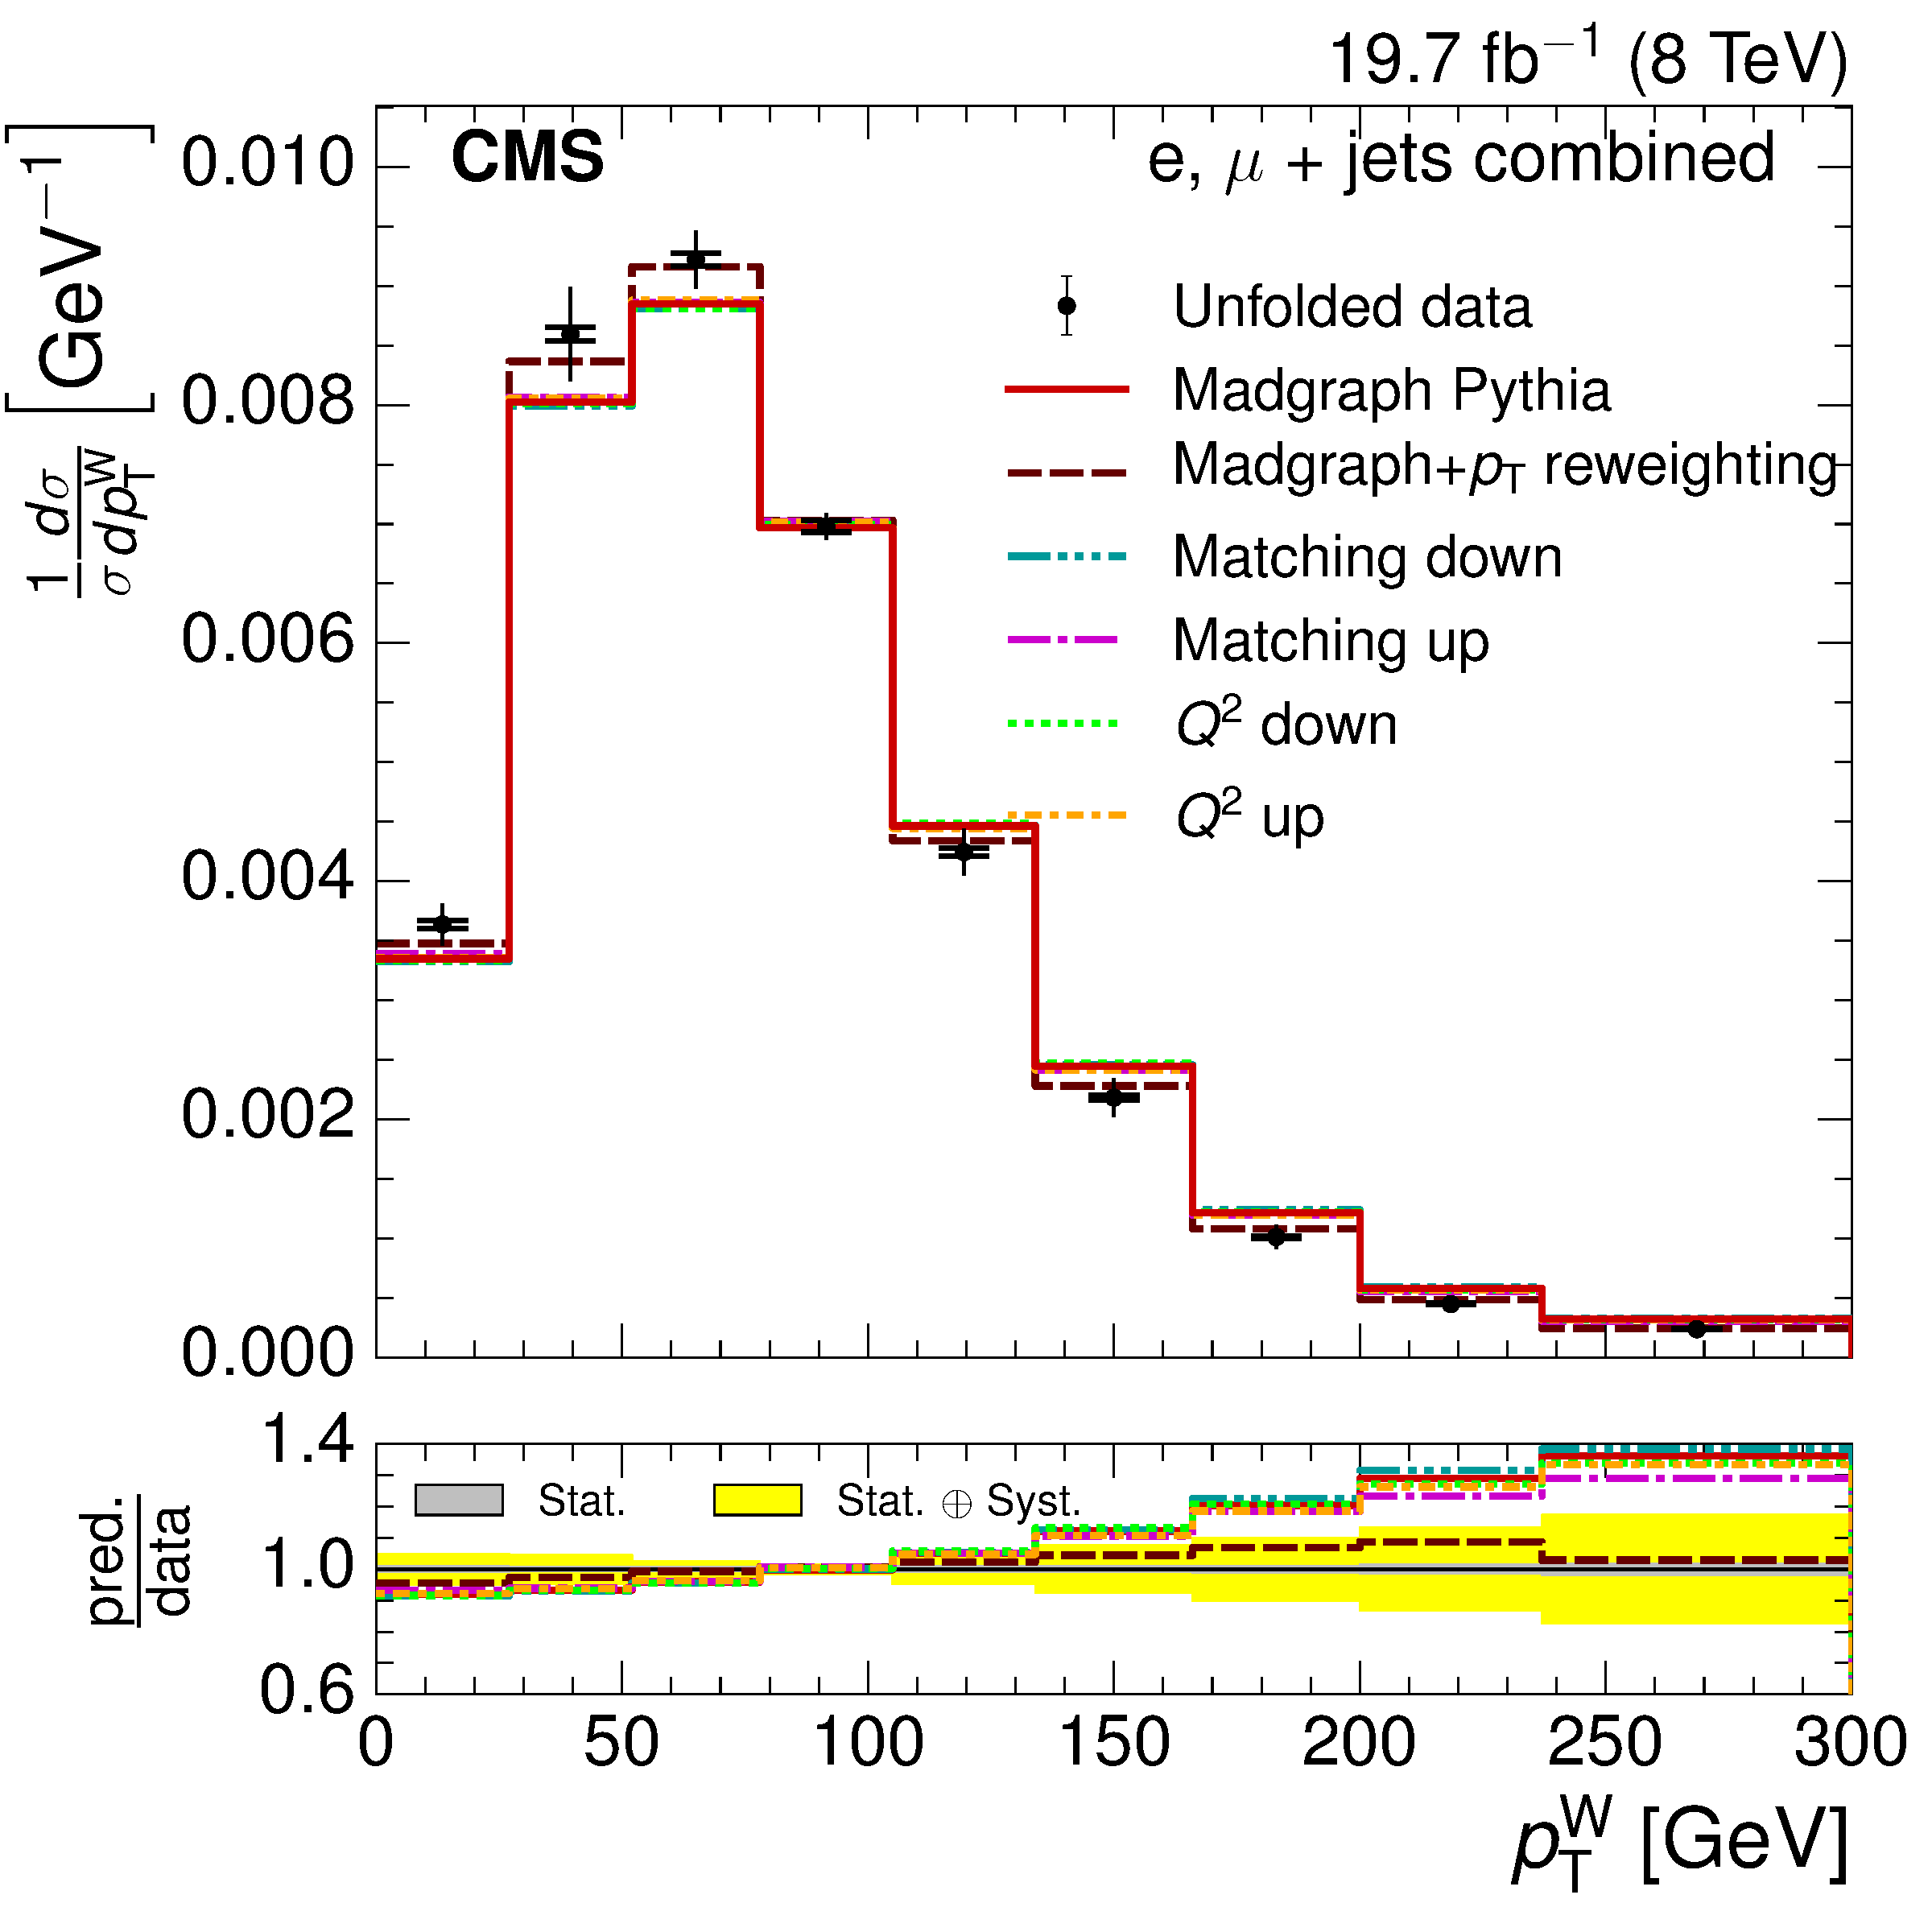
\includegraphics[width=0.48\textwidth]{Chapters/07_08_09_Analysis/Images/results/fit/8TeV/WPT/central/normalised_xsection_combined_systematics_shifts.pdf}\\
     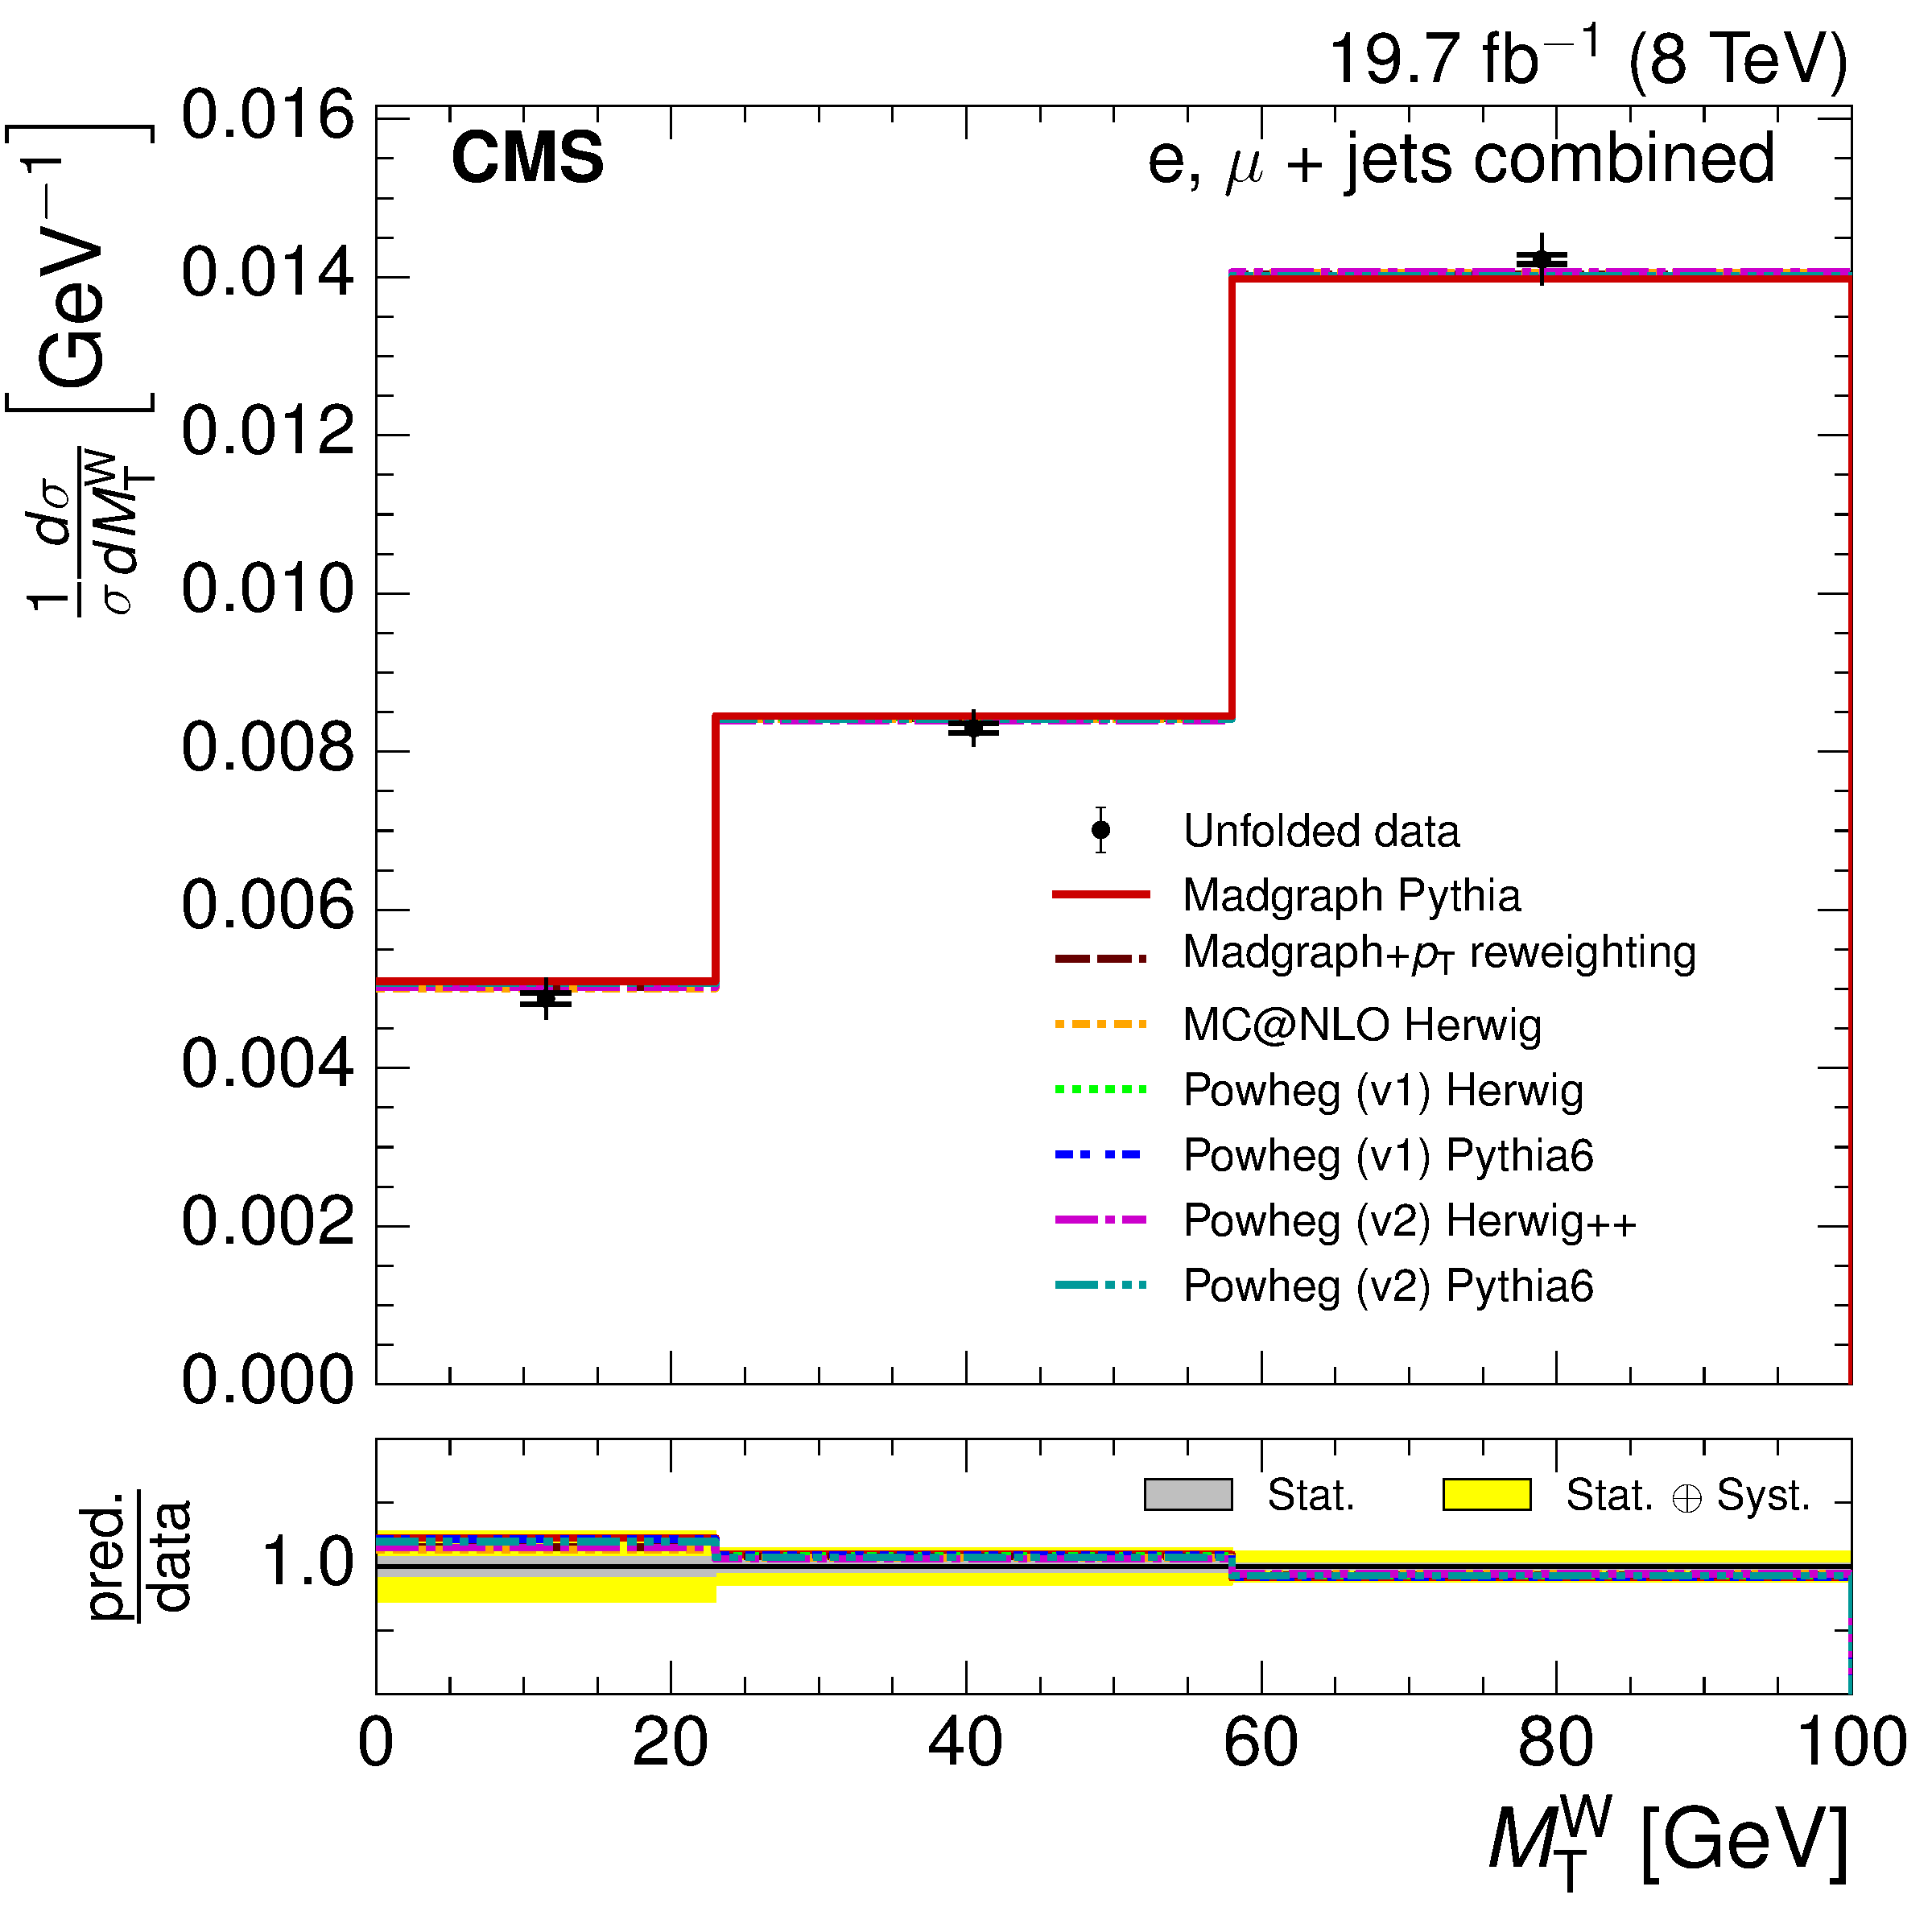
\includegraphics[width=0.48\textwidth]{Chapters/07_08_09_Analysis/Images/results/fit/8TeV/MT/central/normalised_xsection_combined_different_generators.pdf}\hfill
     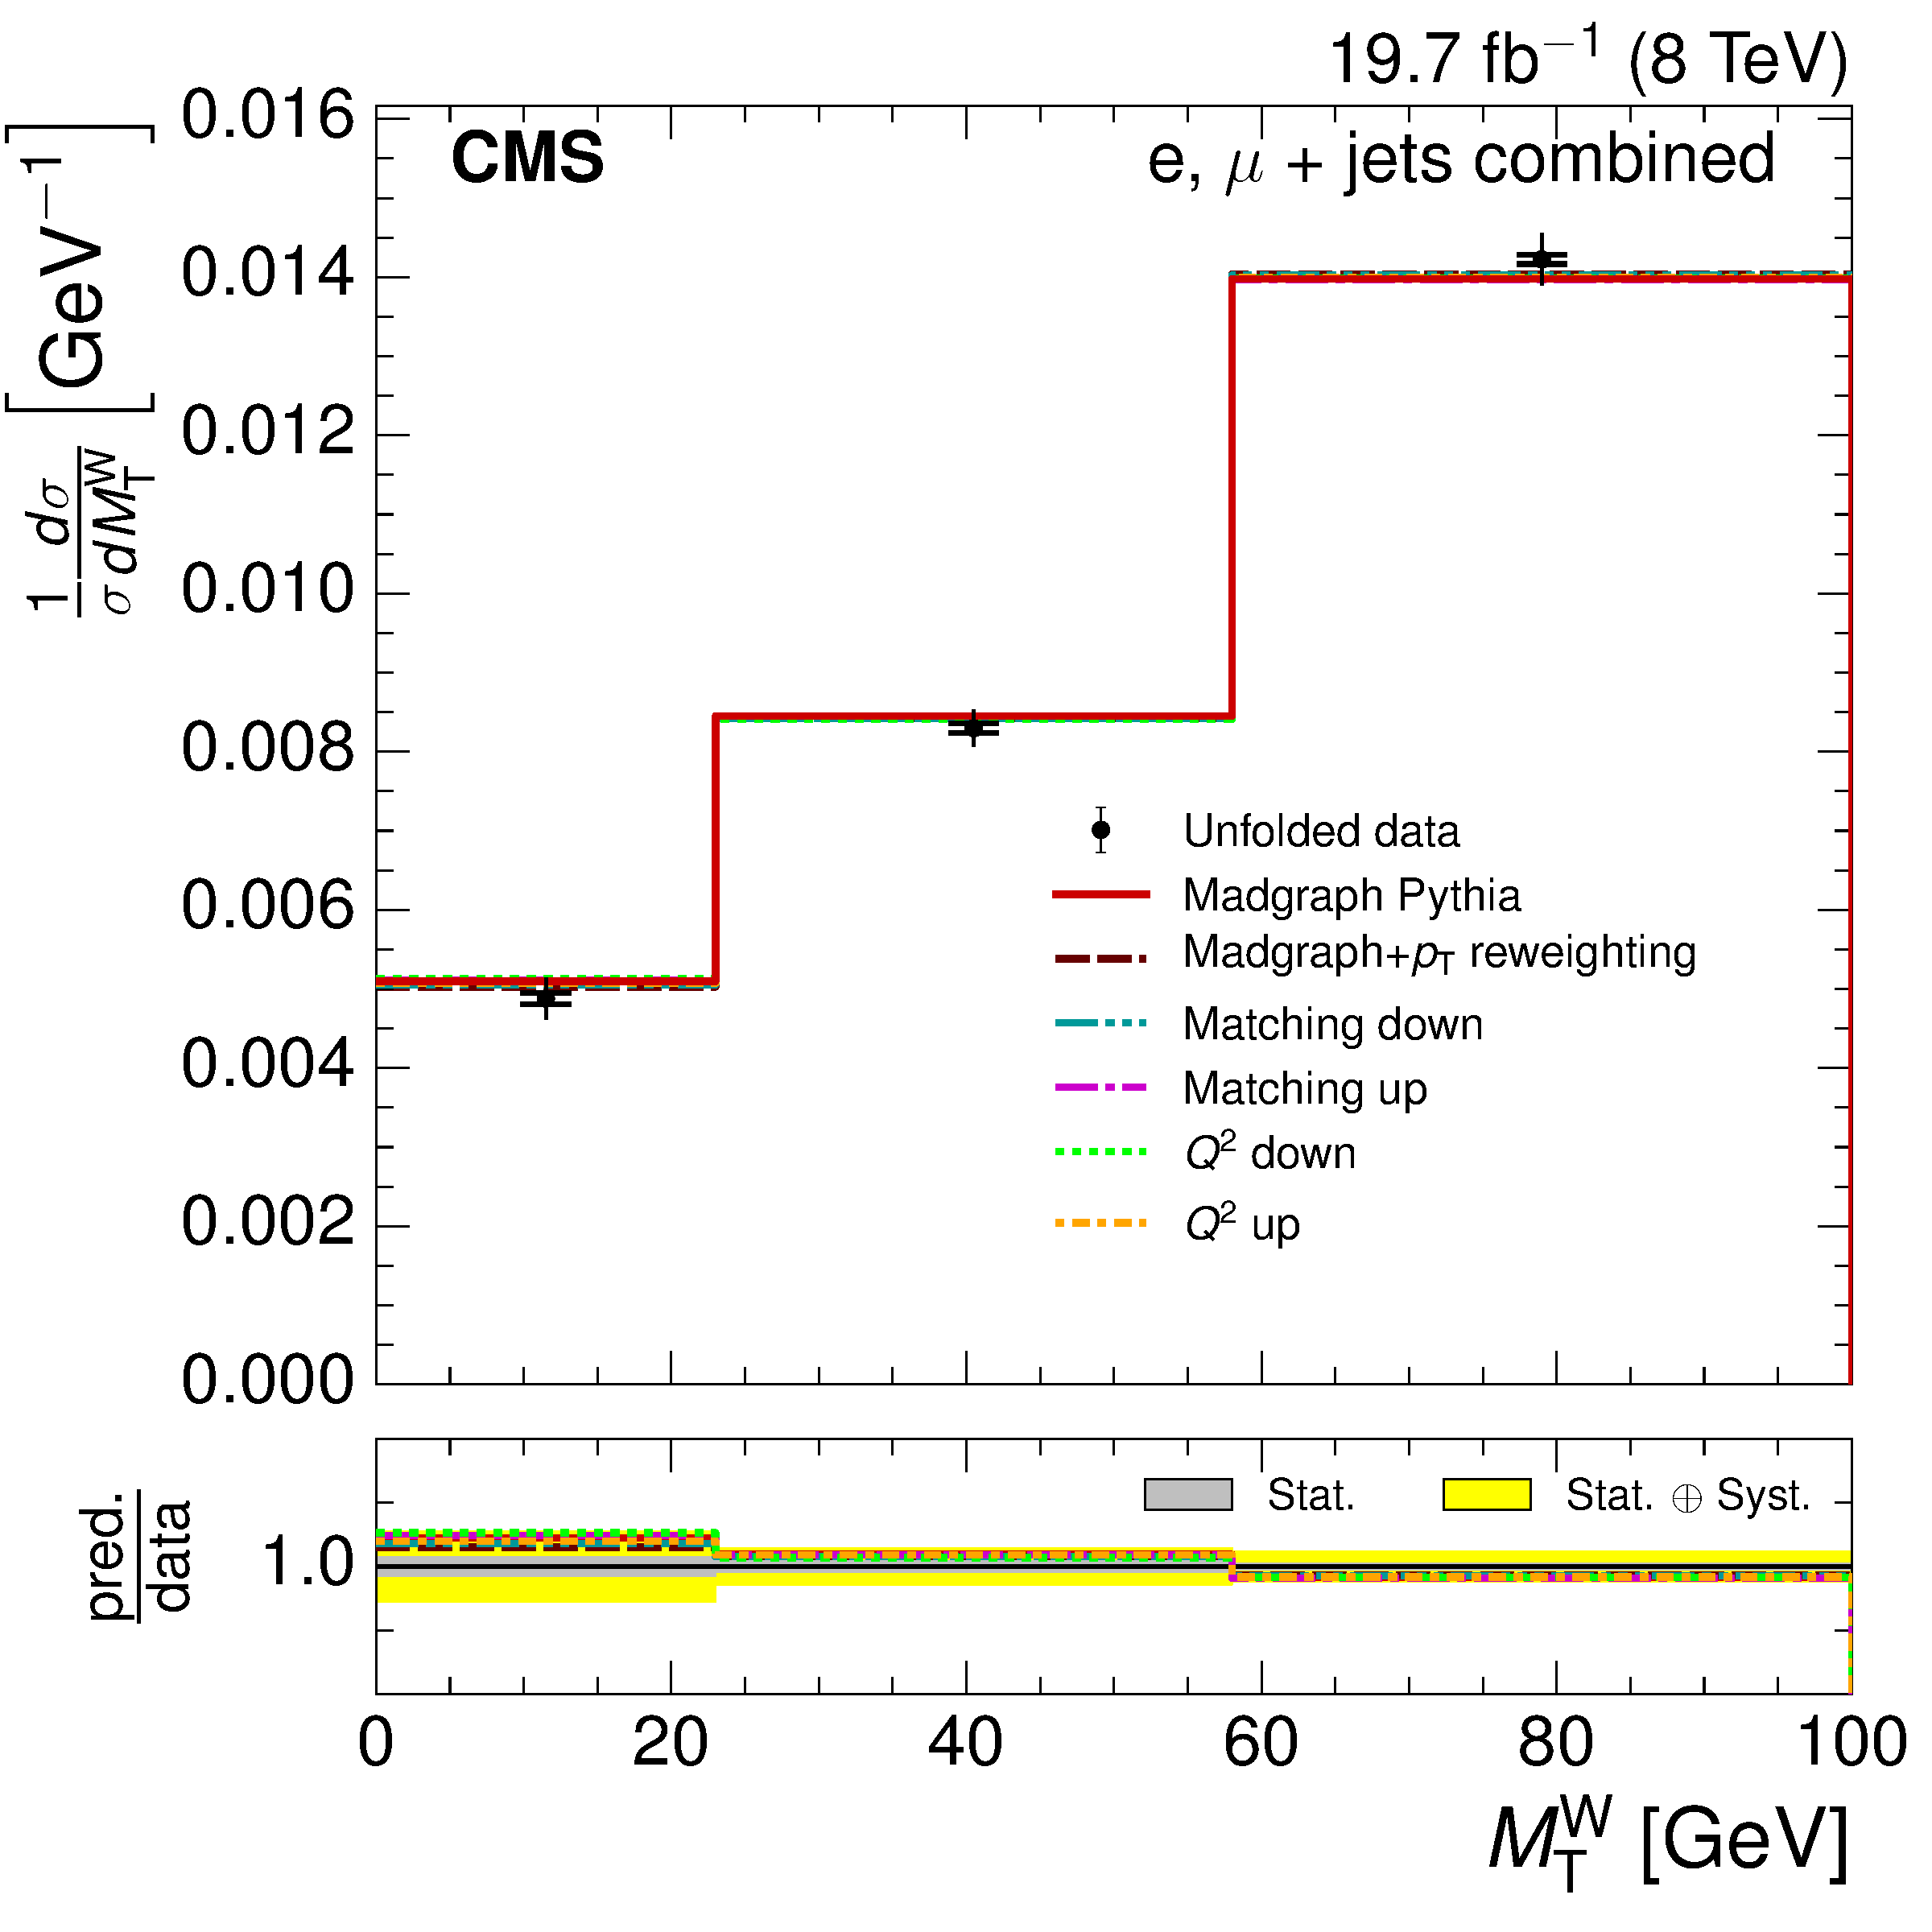
\includegraphics[width=0.48\textwidth]{Chapters/07_08_09_Analysis/Images/results/fit/8TeV/MT/central/normalised_xsection_combined_systematics_shifts.pdf}\\
     \caption[Comparison of the measured normalised differential cross section with respect to \wpt and \mt to
     different Monte Carlo generators and predictions at $\roots=8\TeV$.]{Comparison of the measured
     normalised differential cross section with respect to \wpt (upper) and \mt (lower) to different Monte
     Carlo generators: \MADGRAPH, \POWHEGHERWIG1, \POWHEGPYTHIA1, \POWHEGHERWIG2, \POWHEGPYTHIA2 and \MADGRAPH
     corrected for top \pt mismodelling (left) and to different Monte Carlo predictions matching threshold
     up/down and factorisation scale up/down (right) in the combined electron+jets and muon+jets channel at
     $\roots=8\TeV$. The lower plots show the ratio of the predictions to the data.}
     \label{fig:result_WPT_MT_8TeV_combined}
\end{figure}